\documentclass[a4paper,14pt]{extarticle}
\usepackage[utf8]{inputenc}
\usepackage[english,russian]{babel}

\usepackage{amsthm}
\usepackage{graphicx}
\usepackage{caption}
\usepackage{amssymb}
\usepackage{amsmath}
%%%%%%%%%%%%%%%%
\usepackage{amsfonts} 
%\usepackage[colorlinks=true, allcolors=blue]{hyperref}
%%%%%%%%%%%%%%%%
\usepackage{mathrsfs}
\usepackage{euscript}
%%%%%%%%%%%%%%%%%%%%%%%%
\usepackage{tikz}
\usepackage{pgfplots}
\usepackage{wrapfig}
\usepackage{subfigure}
\usepackage{url}
%%%%%%%%%%%%%%%%%%%%%%%%
\usepackage{graphicx}
\usepackage{subfig}
\usepackage{caption}
\usepackage{color}
\usepackage{bm}
\usepackage{tabularx}
\usepackage{adjustbox}

%%%%%%%%%%%%%%%%%%%%%%%%%%%%%%%%%%%%%%%
\usepackage{pdfpages}
\usepackage{booktabs,dcolumn,caption}      
\usepackage{cleveref} 
%\usepackage{algorithm,algorithmic}
\usepackage{algorithm}
%\usepackage{algorithm2e}
\usepackage{algpseudocode}
%%%%%%%%%%%%%%%%%%%%%%%%%%%%%%%%%%%%%%%

\usepackage[toc,page]{appendix}

\usepackage{comment}
\usepackage{rotating}

% \DeclareMathOperator*{\argmax}{arg\,max}
% \DeclareMathOperator*{\argmin}{arg\,min}

% \newtheorem{theorem}{Теорема}
% \newtheorem{lemma}[theorem]{Лемма}
% \newtheorem{definition}{Определение}[section]

\numberwithin{equation}{section}

\newcommand*{\No}{No.}
\bibliographystyle{gost71u}

\begin{document}

% Титульный лист
%\begin{titlepage}
    	\begin{center}
        		Министерство науки и высшего образования Российской Федерации Федеральное государственное автономное образовательное учреждение высшего образования
       
		«Московский физико-технический институт (национальный исследовательский институт)»

        		Факультет управления и прикладной математики\\
        		Кафедра <<Интеллектуальные системы>>\\
    	\end{center}

    	\vspace{2cm}

    	\begin{center}
       		\Large \bf Анализ свойств локальных моделей в задачах кластеризации временных рядов
    	\end{center}
    
    	\begin{center}
		~\\[-28pt]
		Выпускная квалификационная работа\\
		(бакалаврская работа)
	\end{center}
	
	\vspace{0.1cm}
	    
    \begin{center}
    	\textbf{Направление подготовки:} 03.03.01 Прикладные математика и физика
    \end{center}

   \vspace{0.1cm}

	\begin{flushright}
		\begin{table}[!ht]
			\centering
			\begin{tabular}{l}
				~~~~~~~~~~~~~~~~~~~~~~~~~~~~~~~~~~~~~~~~~~~~~~~~~~ \textbf{Выполнил:}\\
				~~~~~~~~~~~~~~~~~~~~~~~~~~~~~~~~~~~~~~~~~~~~~~~~~~ студент группы 574\\
				~~~~~~~~~~~~~~~~~~~~~~~~~~~~~~~~~~~~~~~~~~~~~~~~~~ Грабовой Андрей Валериевич\\
				~~~~~~~~~~~~~~~~~~~~~~~~~~~~~~~~~~~~~~~~~~~~~~~~~~ \underline{\hspace{7cm}}\\[-10pt]
				\begin{scriptsize}
	    			~~~~~~~~~~~~~~~~~~~~~~~~~~~~~~~~~~~~~~~~~~~~~~~~~~~~~~~~~~~~~~~~~~~~~~~~~~~~~~~~~~~~~~~~~~~~~~~~~~\,
	    			(подпись обучающегося)
	   		 	\end{scriptsize}\\[15pt]
				~~~~~~~~~~~~~~~~~~~~~~~~~~~~~~~~~~~~~~~~~~~~~~~~~~ \textbf{Научный руководитель:}\\
				~~~~~~~~~~~~~~~~~~~~~~~~~~~~~~~~~~~~~~~~~~~~~~~~~~ Доктор физико-математических наук\\
				~~~~~~~~~~~~~~~~~~~~~~~~~~~~~~~~~~~~~~~~~~~~~~~~~~ Стрижов Вадим Викторович\\
				~~~~~~~~~~~~~~~~~~~~~~~~~~~~~~~~~~~~~~~~~~~~~~~~~~ \underline{\hspace{7cm}}\\[-10pt]
				\begin{scriptsize}
					~~~~~~~~~~~~~~~~~~~~~~~~~~~~~~~~~~~~~~~~~~~~~~~~~~~~~~~~~~~~~~~~~~~~~~~~~~~~~~~~~~~~~~~~~~~~
	    			(подпись научного руководителя)
	    		\end{scriptsize}
	    	\end{tabular}
	    \end{table}
	\end{flushright}


	\begin{center}
		Москва 2019
	\end{center}

\end{titlepage}



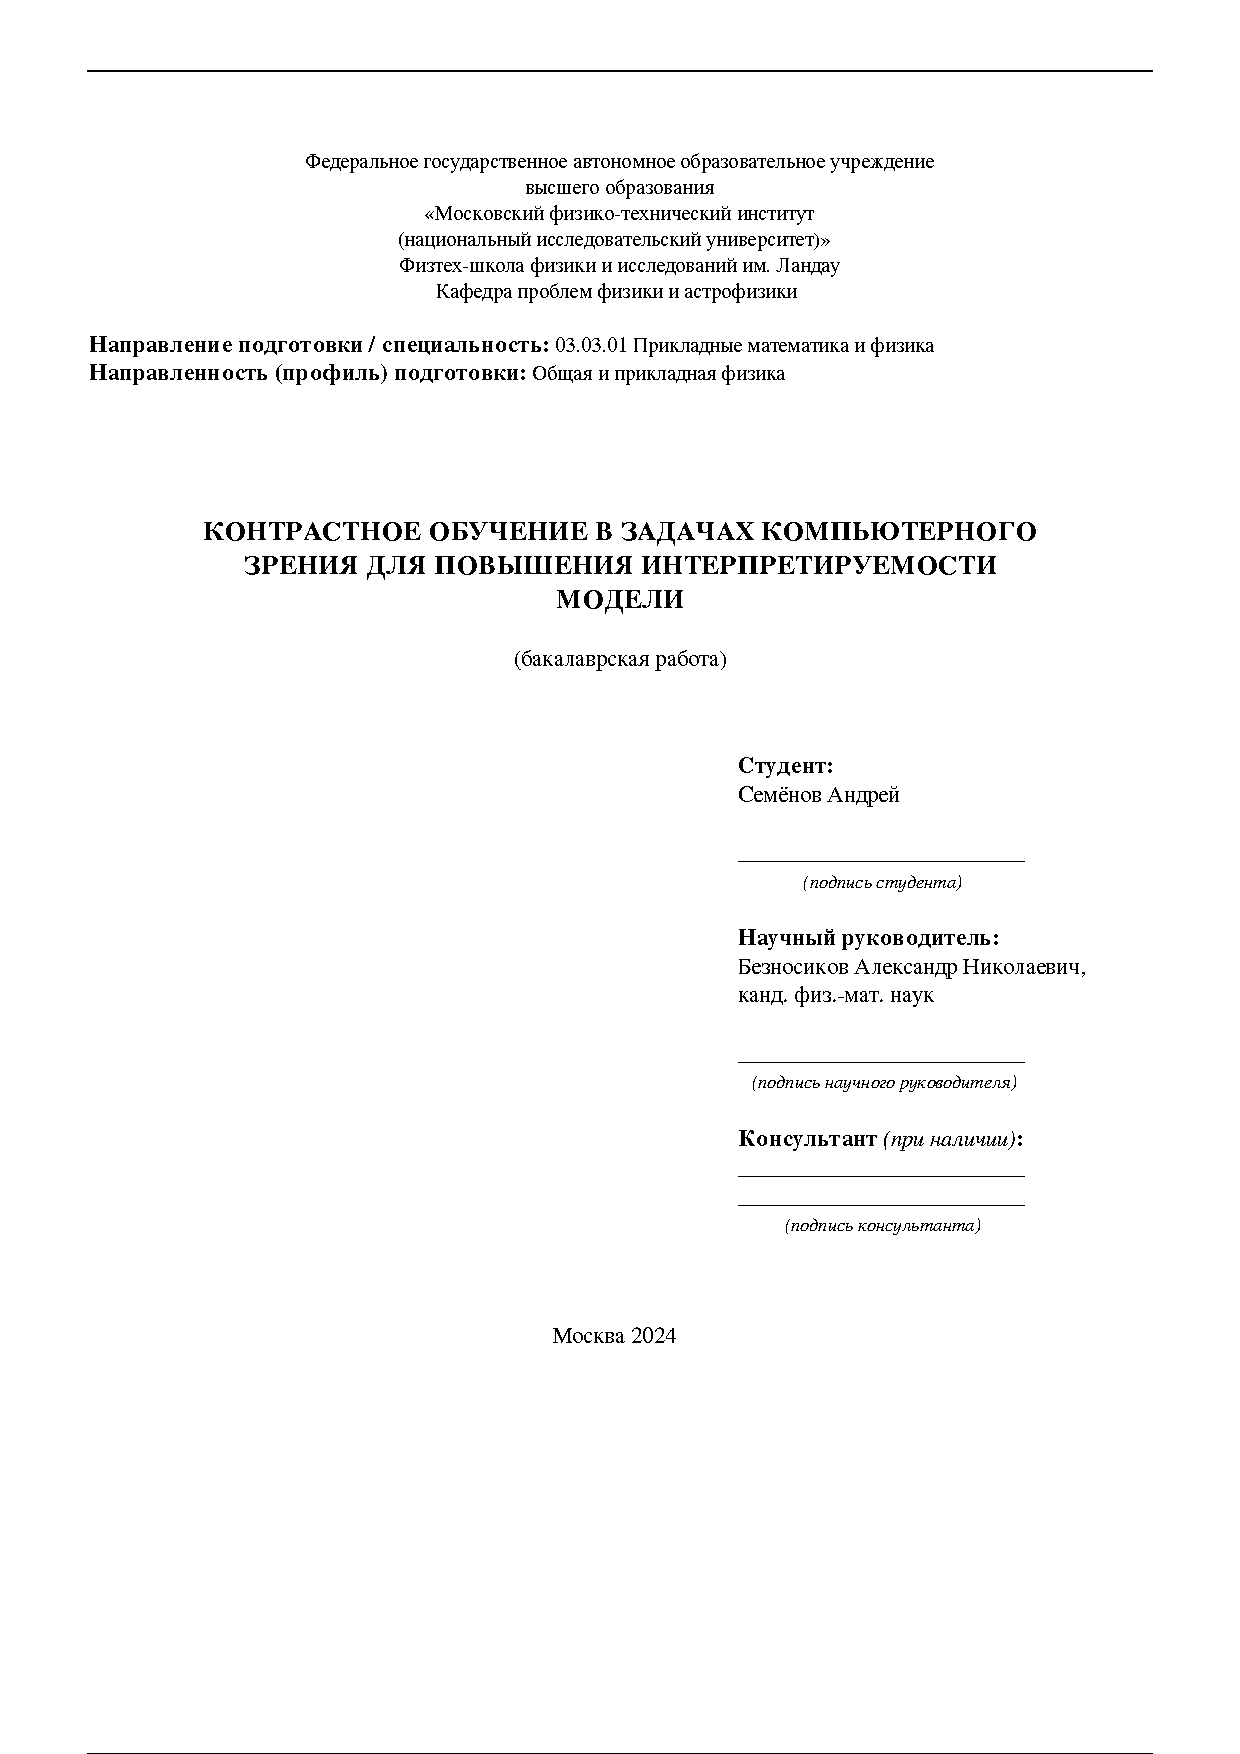
\includepdf[pages=-]{./title.pdf}

% Аннотация
\newpage

\begin{abstract}
Мы предлагаем новую архитектуру и метод объяснимой классификации с использованием концептуальных боттлнек моделей (CBM). В то время как SOTA подходы к задаче классификации изображений работают как черный ящик, растет спрос на модели, которые могли бы предоставлять интерпретируемые результаты. Такие модели часто учатся предсказывать распределение по меткам классов, используя дополнительное описание этих целевых экземпляров, называемое концепциями. Однако существующие методы определения боттлнеков имеют ряд ограничений: их точность ниже, чем у стандартной модели, и CBM требуют дополнительного набора концепций для использования. Мы предоставляем основу для создания концептуальной боттлнек модели на основе предварительно обученного мультимодального энкодера и новых CLIP-подобных архитектур. Представляя новый тип слоев, известный как концептуальные боттлнек слой, мы описываем три метода их обучения: с использованием $\ell_1$-потерь, контрастивных потерь и функции потерь, основанной на распределении Gumbel-Softmax (Sparse-CBM), в то время как конечный слой FC по-прежнему обучается с использованием перекрестной энтропии. Мы демонстрируем значительное повышение точности при использовании разреженных скрытых слоев в CBM на основе CLIP. Это означает, что разреженное представление вектора активации концепций имеет смысл в CBM. Более того, с помощью нашего алгоритма поиска по матрице концепций мы можем улучшить предсказание CLIP в сложных наборах данных без какого-либо дополнительного обучения или файн-тьюнинга. Код доступен по ссылке: \texttt{https://github.com/Andron00e/SparseCBM}.
\end{abstract}






% Нумерация должна начинаться со второй страницы
\setcounter{page}{2}

% Оглавление
\newpage
\tableofcontents

% Обозначения и сокращения
% \input{./dict.tex}

\newpage


\section{Введение}
\label{submission}

В последние годы SOTA \cite{yu2023noisynn}-подходы к классификации изображений достигли значительных показателей точности. Основным бенчмарком для проверки качества таких моделей является ImageNet LSVRC \cite{russakovsky2015imagenet}, а наиболее продвинутые модели обучаются от нескольких недель до месяцев на таких масштабных датасетах, как JFT-300M \cite{sun2017revisiting} и ImageNet-21K \cite{5206848} на множестве GPU-машин. Хотя классические современные решения, такие как ViT \cite{dosovitskiy2021image} и другие модели Vision Transformer, превосходят решения на основе ResNet \cite{he2015deep}, хотя для предварительного обучения требуется значительно меньше вычислительных ресурсов, они по-прежнему работают как черный ящик. Получив на вход мини-пакет изображений и необходимые метки, они выдают готовое распределение по меткам классов. В этом случае целью подхода Concept Bottleneck Models \cite{koh2020concept} является разработка моделей, которые бы отвечали на такие вопросы, как: "Почему вы выбрали именно этот класс?", "На основании каких результатов вы его предсказали?". Предполагается, что этот подход будет чрезвычайно полезен в областях, где объяснения имеют решающее значение, например в медицинских приложениях. 

\begin{figure}[t]
\begin{center}
\centerline{
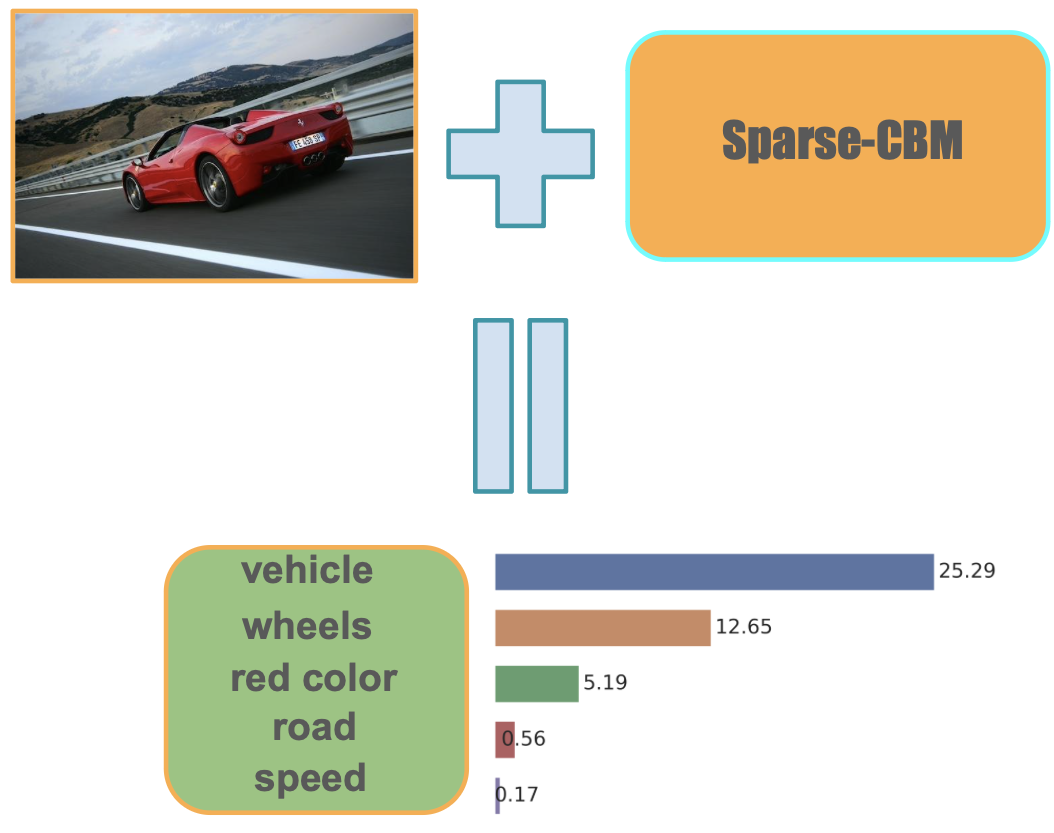
\includegraphics[width=0.55\columnwidth]{./figures/opening_test_3.png}}
\caption{Пример концептов, отобранных Sparse-CBM.}
\label{fig:opening}
\end{center}
\vskip -0.4in
\end{figure}
Мы изучаем модели, которые сначала предсказывают промежуточный набор понятных человеку понятий, а затем используют его для предсказания конечной метки, поддерживаемой выбранными понятиями. Построение интерпретируемых нейронных сетей стало более популярным с представлением модели OpenAI CLIP \cite{radford2021learning} и развитием методов контрастивного обучения \cite{aljundi2022contrastive}. Нельзя не отметить растущее направление мультимодальности \cite{reed2022generalist,chen2023sharegpt4v} с его многообещающими результатами по объединению нескольких модальностей, таких как текст, аудио, видео, для построения одной модели, способной решать множество последующих задач. Исследования моделей Concept Bottleneck и Contrastive Learning также подразумевают мультимодальность (между парами изображение-текст) как в контролируемых \cite{khosla2021supervised}, так и в неконтролируемых \cite{gao2022simcse} условиях, и даже могут пригодиться для приложений Reinforcement Learning \cite{srinivas2020curl}.

\subsection{Контрастное обучение}

Наша работа основана в основном на подходах Contrastive Representation Learning к задаче классификации, когда основной целью является изучение пространства вкраплений таким образом, чтобы схожие образцы сближались, а несхожие отдалялись друг от друга. В случае контрастивного обучения мы стремимся выучить совместное латентное пространство вкраплений изображений и текста, как это делают CLIP, ALIGN \cite{jia2021scaling}, BLIP \cite{li2022blip} и LiT \cite{zhai2022lit}.
% (с настройкой только текстовой модели) do. 
Контрастные потери на основе softmax \cite{1467314} стали ключевой задачей предварительного обучения таких моделей. Однако недавняя работа \cite{zhai2023sigmoid} показала возможность превзойти предыдущие результаты с предварительным обучением на основе сигмоидальных потерь, что требует значительно меньше памяти и, таким образом, позволяет обучать модель заблокированного изображения из \cite{zhai2022lit} с гораздо большим размером партии. Большинство методов контрастного обучения применяются для увеличения объема данных, но не только для изображений в компьютерном зрении. Предыдущие работы \cite{wei2019eda,kobayashi2018contextual,fang2020cert,shen2020simple} показали, как текст может быть дополнен без изменения всей семантики предложения.

\subsection{Классификация с Concept Bottleneck}\label{sec:bottls}

Введенные \cite{koh2020concept}, модели узких мест концепций стали популярным направлением в объясняемом ИИ. Общая идея и конвейер обучения узких мест довольно интуитивны: вместо того чтобы решать интересующую задачу напрямую, давайте разделим основную проблему на более мелкие части и извлечем из них наиболее значимые понятия. В качестве концептов можно рассматривать любую понятную человеку информацию. Например, пытаясь классифицировать сломанную руку, хирург-ортопед ищет особые зрительные паттерны, например, трещины на костях, нереальные изгибы рук и т. д. CBM обучаются сначала предсказывать понятные человеку концепции, а затем принимать окончательное решение на основе полученных концепций. Примечательно, что именно для этих целей сквозное обучение не является обязательным, многие предыдущие работы, на которые мы ссылаемся в разделе \ref{sec:relwork}, представляют свои фреймворки для построения CBM на основе существующих предварительно обученных признаков-экстракторов. В чем преимущество CBM, если точность ухудшилась по сравнению с обычным классификатором? Снижение производительности, безусловно, является ключевой проблемой для узких мест в CBM, но вместо этого мы пытаемся использовать этот параметр для определения компромисса между точностью модели и ее интерпретируемостью. Ограничив модель промежуточным набором концепций и конечными предсказаниями слоя с полным подключением (FC), мы можем: 

\begin{description}
\item \underline{Объяснить}, какую информацию модель воспринимает как более/менее важную для классификации входных данных.
\item \underline{Понять}, почему модель совершает конкретную ошибку: определить, каким понятиям был отдан неверный приоритет.
\end{description}

За вышеперечисленными преимуществами общих Concept Bottleneck моделей следуют ключевые ограничения:
\begin{description}
\item \underline{Подготовка концептов:} Для обучения CBM требуются метки, помеченные дополнительными понятиями, сбор которых занимает много времени и стоит дорого.
\item \underline{Производительность:} На практике использование моделей, точность которых ниже, чем у неограниченных, неперспективно.
\item \underline{Редактирование модели:} Общая проблема, возникающая в подходе Concept Bottleneck Model, - невозможность целостного вмешательства в саму модель. Предыдущие работы \cite{yuksekgonul2023posthoc} демонстрируют методы обратной связи, управляемой человеком, а \cite{oikarinen2023labelfree} полагается на TCAV\cite{kim2018interpretability}, которая все еще обращает внимание на локальные ошибки модели в случае, когда МД не изучается сквозным образом. В то время как обычно пользователи хотят получить предварительно обученную CLIP-подобную модель и создать над ней "узкое место". Поэтому этот вопрос все еще остается открытым.
\end{description}

\subsection{Наш вклад}

В этой статье мы вносим вклад в лучшее понимание последних подходов к классификации изображений с помощью CBM. В частности, мы раскрываем возможности CBM, обученных самоконтролем, и обнаруживаем значительный рост производительности моделей, генерирующих разреженное внутреннее представление. Мы стремимся раскрыть ранее скрытые возможности необработанных CLIP подобных моделей с помощью представленного в разделе \ref{sec:cms} алгоритма "нулевого обучения" с предложенным в разделе \ref{sec:framework} фреймворком. Только используя оценки точечных продуктов CLIP, мы можем сделать нашу модель более интерпретируемой в смысле опоры на промежуточный набор понятий. Кроме того, все наши подходы поддерживают ручную генерацию концептов. Мы формулируем наш дальнейший фреймворк как частный случай контрастной тонкой настройки, когда предварительно обученные модели затем тонко настраиваются с помощью контрастных объективных функций \cite{weng2021contrastive}.  

Вместо того чтобы разрабатывать архитектуры для конкретных случаев, мы ищем алгоритмы контрастной тонкой настройки, которые могут работать с общими рамками создания Concept Bottleneck из предварительно обученного мультимодального кодера. Кроме того, наш подход опирается на некоторые ранее представленные схемы с изменением целей, для которых обучаются скрытые слои. Примечательно, что, поскольку структура магистральной модели хорошо распараллеливается, наши CBM можно относительно легко поддерживать вертикальным или информационным параллелизмом. Это позволяет нам спроектировать узкое место, которое может решать свою задачу более эффективно.

Мы резюмируем основной вклад нашей работы следующим образом:

\textbf{(\underline{Вклад 1})} Мы формально определяем алгоритм для повышения точности CLIP и в то же время делаем модель более интерпретируемой. Мы также приводим анализ латентного пространства CLIP и рассказываем, как концепции влияют на него. 

\textbf{(\underline{Вклад 2})} На основе проведенного анализа мы формулируем фреймворк для построения CBM: новую архитектуру и метод обучения, включающий контрастную тонкую настройку дополнительных слоев. Мы реализуем автоматическую генерацию набора концептов на основе предоставленного набора данных и контрастных вариантов наших функций потерь, таким образом, наш фреймворк облегчает обучение новых слоев.

\textbf{(\underline{Вклад 3})} Мы продемонстрировали эффективность метода Sparse-CBM (см. раздел \ref{sec:sparsecbm}), запустив нашу архитектуру на наборах данных ImageNet \cite{russakovsky2015imagenet}, CUB-200 \cite{wah_branson_welinder_perona_belongie_2011}, Places365 \cite{7968387}, CIFAR100 и CIFAR10 \cite{krizhevsky2009learning}. В результате Sparse-CBM превосходит предыдущую безлаберную \cite{oikarinen2023labelfree} работу на нескольких из них и достигает точности 80,02\% на CUB-200.

\section{Сопутствующие работы}
\label{sec:relwork}

Подходы к классификации изображений с использованием концептуальных моделей - быстро развивающаяся область, поскольку в разделе \ref{sec:bottls} упоминаются преимущества их возможностей для интерпретации, то уже было представлено множество достаточных методов. В ранних работах \cite{koh2020concept,losch2019interpretability,Marcos_2020_ACCV} предлагается обучать CNN \cite{5537907} и создавать дополнительный слой перед последним полностью связанным слоем, где каждый нейрон соответствует интерпретируемому человеком понятию. Поскольку модели "узкого места" страдают от необходимости подготовки набора концепций, поиск эффективного метода создания набора поддерживаемых концепций является необходимой задачей. В предыдущих работах по безэтикетному, постхоковому CBM и LaBo \cite{oikarinen2023labelfree,yuksekgonul2023posthoc,yang2023language} прослеживается тенденция к созданию фреймворков (как преобразовать существующую модель в модель узкого места) вместо того, чтобы изучать модели с нуля. Они также показывают методы создания набора достаточных концептов и вводят новые метрики в классификацию с помощью CBM. Поскольку хорошо подготовленный набор концептов является ключевым ингредиентом проблемы CBM, \cite{schwalbe2022concept} предлагает общий обзор методов, использующих вкрапления концептов.Помимо прочего, авторы \cite{oikarinen2023labelfree} обучают модель по двум алгоритмам: голова классификатора с решателем GLM-SAGA \cite{pmlr-v139-wong21b} и узкие слои с вариантами косинусного сходства, что близко к нашему конвейеру. \cite{menon2022visual} сообщают о методе, который не требует обучения базовой модели, вместо этого они запрашивают у CLIP определенный паттерн и находят конечный класс с помощью предложенной формулы, а \cite{oikarinen2023clipdissect} предлагает способ описания нейронов скрытых слоев CLIP. \cite{gao2022pyramidclip} предлагает построить входную пирамиду с различными семантическими уровнями для каждой модальности и объединить визуальные и лингвистические элементы в иерархию, что удобно для обнаружения объектов. \cite{pmlr-v139-wong21b} предлагает идею сохранить конечный слой FC разреженным, что делает его более интерпретируемым. \cite{kazmierczak2023clipqda} вмешивается в латентное пространство CLIP и показывает, что оно может быть эффективно смоделировано как смесь гауссианов. Также отметим, что в недавней работе \cite{Alukaev_2023} предлагается использовать сигмоид Гумбеля после экстракторов признаков (для концептов и изображений), которые дают разреженное представление концептов. Идея разреженности также находит свое продолжение в работе \cite{panousis2023discover}, где авторы представляют новый тип слоев Local Winner-Takes-All \cite{panousis2019nonparametric}, основанных на активационной разреженности. Предыдущие работы по разреженности также схожи с нашей, но мы, в свою очередь, создаем варианты контрастных потерь для обучения CBM.

\vspace{-0.3cm}
\section{Предварительная информация}\label{sec:prel}
\vspace{-0.2cm}

В этом разделе мы приводим все обозначения, необходимые для представления наших методов обучения моделей Concept Bottleneck.

\paragraph{Нотация.}\label{sec:notation} В основном мы работаем с OpenAI CLIP, он состоит из двух кодировщиков, один для изображений, другой для текста. Эти кодировщики позволяют нам получить векторное представление для обоих типов данных в многомерном пространстве одной и той же размерности (обычно 512). Поэтому мы используем следующие обозначения. Мы называем $f_{\mathrm{T}}(t, \theta)$ выходом текстового кодера $f_{\mathrm{T}}$, то есть вкраплениями текста из партии текстовых примеров $t$. Под $\theta$ мы понимаем параметры текстового кодера, если он не поддается обучению, то мы опускаем эти параметры. Также, поскольку в большинстве экспериментов мы настраиваем лишь небольшое количество весов исходной модели CLIP (см. \cref{tab:backbone_nets}), а полностью обучаем только новые встроенные слои, для простоты мы указываем веса $\theta$ с одинаковым символом для обоих кодеров. Получив мини-пакет изображений $x$, мы используем $f_{\mathrm{I}}(x, \theta)$ для кодировщика изображений $f_{\mathrm{I}}$ на выходе, т.е. вкраплений входных изображений, каждое размерностью 512 для основных конфигураций модели CLIP. $\langle , \rangle$ обозначает скалярное (точечное) произведение, через $\times$ мы обозначаем декартово произведение двух множеств. Для векторов $\|z\|$ - это норма на векторном пространстве, которому принадлежит $z$. Как правило, под этим обозначением подразумевается $2$-норма для векторов из $\mathbb{R}^{n}$ или норма Фробениуса для матриц из $\mathbb{R}^{m\times n}$, если не указано иное.
\section{Постановка задачи и основные Результаты}
\label{sec:probl}

В этом разделе мы представляем наш алгоритм и фреймворк для построения CBM. Алгоритм, представленный в разделе \ref{sec:cms}, обеспечивает повышение точности CLIP наряду с его интерпретируемостью, а фреймворк (см. раздел \ref{sec:framework}) обеспечивает контрастную тонкую настройку магистрального бимодального кодера.

\subsection{Постановка задачи}

Наряду с задачей классификации изображений, мы формализуем классификацию с помощью \textbf{Concept Bottleneck}. Учитывая кодировщики изображений и текста, мы намерены выучить дополнительную проекцию из пространства вложений, предоставляемого кодировщиками, в векторное пространство, соответствующее представлению концептов изображений, а затем выучить окончательную проекцию для получения вероятностей меток классов. Мы намерены выучить следующее отображение: $x\times t \to \omega \to l$, согласно \textit{Notation} \ref{sec:notation}: $x$ обозначает область изображений, $t$ - текстовые понятия, а $\omega$ и $l$ - представление понятий и метки классов соответственно. Это отличается от стандартной схемы $x\to \omega\to l$ тем, что мы можем создавать концепты $t$ автоматизированным способом.

\subsection{Concept Matrix Search algorithm}\label{sec:cms}

Мы представляем алгоритм Concept Matrix Search (CMS), который использует возможности CLIP для представления изображений и текстов в совместном латентном пространстве одной и той же размерности. Сначала мы формулируем гипотезу о наших данных, принимая во внимание то, как обучена основная модель CLIP.

Определим набор эмбеддингов картинки как $\mathrm{I} = \{i_1, \dots, i_{|\mathrm{I}|}\}$, where $i_{\mathrm{k}} = f_{\mathrm{I}}(x_{\mathrm{k}}, \theta)$. И в качестве $\mathrm{D} = \{d_1, \dots, d_{|\mathrm{D}|}\}$ мы определим набор эмбеддингов концептов, $d_\mathrm{j} = f_{\mathrm{T}}(\mathrm{concept}_{\mathrm{j}}, \theta)$, тем временем $\mathrm{C} = \{c_1, \dots, c_{|\mathrm{C}|}\}$ набор эмбеддингов классов, где эмбеддинги меток этих классов похоже выражены iв терминах $f_{\mathrm{T}}$. Мы также определим две матрицы для которых наша модель будет вычислять попарную близость картинка-текст:

Image-Concept matrix (V-matrix): $\mathcal{V}\in \mathbb{R}^{|\mathrm{I}|\times|\mathrm{D}|}$, such that $\mathcal{V}_{\mathrm{kl}} =\langle i_\mathrm{k}, d_\mathrm{l}\rangle$.

Class-Concept matrix (T-matrix): $\mathcal{T}\in\mathbb{R}^{|\mathrm{C}|\times|\mathrm{D}|}$, such that $\mathcal{T}_{\mathrm{kl}} = \langle c_\mathrm{k}, d_\mathrm{l} \rangle$.

Теперь мы можем сформулировать \textit{гипотезу} лежащую в основынии CMS.

\paragraph{Гипотеза.}

Для $f_{\mathrm{I}}(x,\theta)$ and $f_{\mathrm{T}}(t,\theta)$ определим косинусную близость как:
\[ 
\cos(f_{\mathrm{I}}(x, \theta), f_{\mathrm{T}}(t, \theta)) = \frac{\langle f_{\mathrm{I}}(x, \theta), f_{\mathrm{T}}(t, \theta) \rangle}{\|f_{\mathrm{I}}(x, \theta)\| \|f_{\mathrm{T}}(t, \theta)\|}_.
\]

Тогда,
\begin{quote}
\textit{Для матриц} $\mathcal{V}$, $\mathcal{T}$ \textit{и функции} $\phi(\mathrm{m})\colon \mathbb{N}^{|\mathrm{I}|} \to \mathbb{N}^{|\mathrm{C}|}$ \textit{которая отображает индекс эмбеддинга картинки} $\mathcal{V}$ \textit{в индекс его класса из} $\mathcal{T}$\textit{, мы предполагаем:}
\[
\forall \mathrm{j}\neq \mathrm{k} \hookrightarrow \cos(\mathcal{V}_{\mathrm{k},\cdot}^\top, \mathcal{T}_{\phi(\mathrm{k}),\cdot}^\top) \geq \cos(\mathcal{V}_{\mathrm{k},\cdot}^\top, \mathcal{T}_{\phi(\mathrm{j}),\cdot}^\top)_,
\]
\textit{где} $\mathcal{V}_{\mathrm{k},\cdot}$, $\mathcal{T}_{\mathrm{k},\cdot}$ \textit{k-ые строки} $\mathcal{V}$, $\mathcal{T}$ \textit{соответственно.}
\end{quote}

Проще говоря, \textit{гипотеза} гласит, что для всех возможных классов вектор сходства между истинным классом и всеми концептами должен быть наиболее близок к вектору сходства образа этого самого класса и всех концептов. Вектор $\mathcal{V}_{\mathrm{k},\cdot}^\top$ получается путем вычисления косинуса сходства между эмбеддингами $i_{\mathrm{k}}$
и каждым из вложений концепта в $\mathrm{D}$.

\paragraph{CMS алгоритм.}  Сформулировав \textit{гипотезу}, мы предлагаем эффективный метод ее проверки с помощью \cref{Alg:CMS}. Для сокращения вычислительных затрат и памяти мы предлагаем в \cref{Alg:CMS} обрабатывать матрицу $\mathcal{V}$ партиями с размером партии $|\mathrm{B}|<|\mathrm{I}|$. Обратите внимание, что на самом деле мы не выполняем два цикла, а используем эффективное умножение матриц, реализованное в PyTorch \cite{paszke2019pytorch}.

\begin{algorithm}[tb]
    \caption{\textsc{Concept Matrix Search}}
    \label{Alg:CMS}
    \begin{algorithmic}[1]
        \State {\bfseries Input:} Batch of image embeddings $\mathrm{I_{|\mathrm{B}|}}$,  labels, all classes $\mathrm{C}$ and concepts $\mathrm{D}$ embeddings.
            \State Build $\mathcal{V} \in \mathbb{R}^{|\mathrm{B}|\times |\mathrm{D}|}$, $\mathcal{T} \in \mathbb{R}^{|\mathrm{C}|\times |\mathrm{D}|}$ matrices, store $\mathcal{T}$.
            \For{$\mathrm{k}=0,1,2,\dots,|\mathrm{B}|-1$}
                \For{$\mathrm{m}=0,1,2,\dots,|\mathrm{C}|-1$}
                    \State Compute and store $\cos(\mathcal{V}^\top_{\mathrm{k},\cdot}, \mathcal{T}^\top_{\mathrm{m},\cdot})$
                \EndFor
                \State Find $\mathrm{m}_{\mathrm{max}}=\underset{\mathrm{m}}{\operatorname{max}}\cos(\mathcal{V}^\top_{\mathrm{k},\cdot}, \mathcal{T}^\top_{\mathrm{m},\cdot})$
                \If{$\mathrm{label}(\mathrm{k}) = \mathrm{m}_{\mathrm{max}}$}
                    \State the hypothesis has been proven, increase Accuracy
                \Else
                    \State the hypothesis has been disproved
                \EndIf
            \EndFor
            \State \Return Mean accuracy
    \end{algorithmic}
\end{algorithm}

Предлагаемый алгоритм обеспечивает повышение интерпретируемости исходной модели CLIP, не требуя дополнительного обучения. Простую демонстрацию нашего метода можно увидеть на рисунке \cref{fig:cms_example}. В этой работе мы также обнаружили влияние набора концептов на точность CMS, которое представлено на рисунке \ref{fig:cms_acc} и обсуждается в экспериментах (см. раздел \ref{sec:cmsexp}). Мы также представляем эмпирическое подтверждение гипотезы CMS \textit{гипотеза}, рассматривая точность классификации каждого класса отдельно, и показываем явную зависимость от набора концепций \footnote{\url{https://github.com/anonymousedauthor/SparseCBM/blob/main/additional_evaluations/cms_empirical_evidence.ipynb}}.

\subsection{Наш фреймворк для CBMs}
\label{sec:framework}
\begin{figure*}[t]
\begin{center}
\centerline{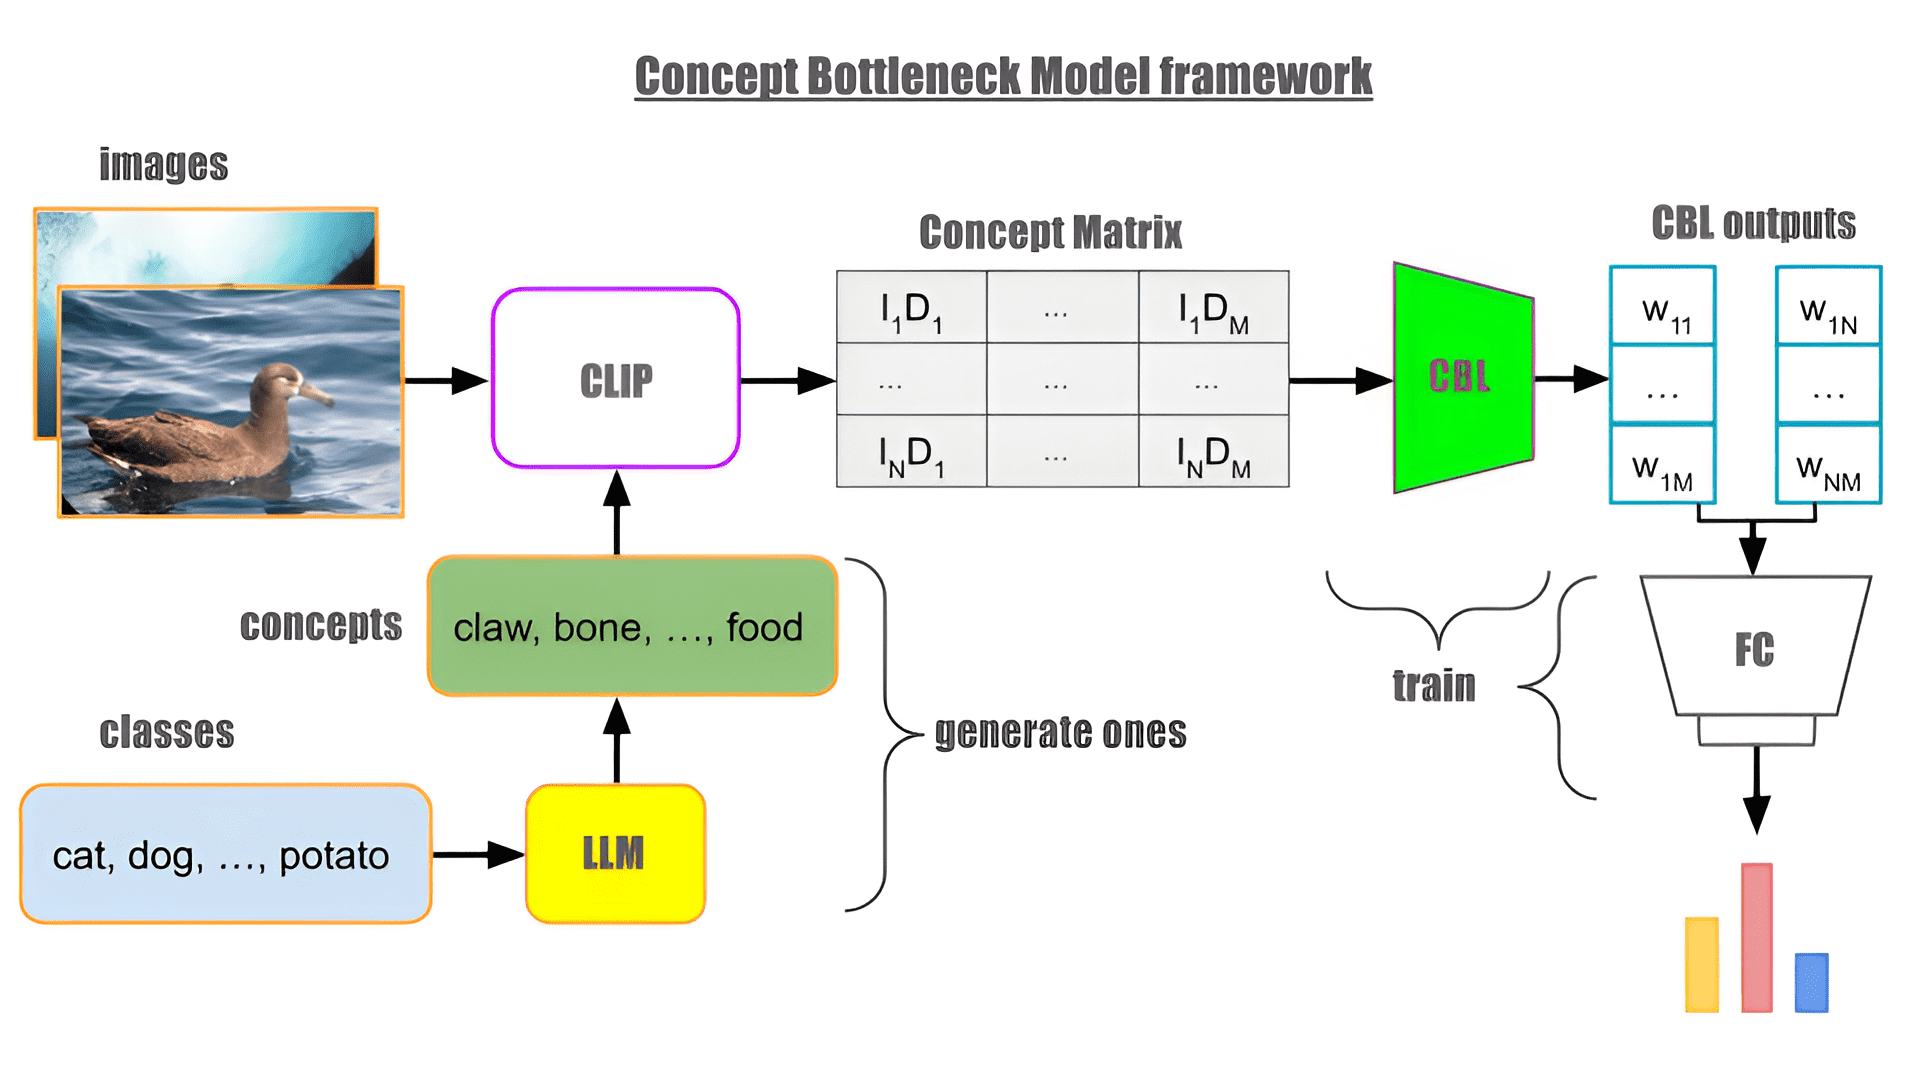
\includegraphics[width=1.\columnwidth]{./figures/framework-compressed.png}}
\caption{Архитектура фреймворка для построения CBM.}
\label{fig:framework}
\end{center}
\end{figure*}

В этом разделе мы предлагаем структуру, которая создает
Concept Bottleneck Model из предварительно обученного мультимодального кодера эффективным способом с минимальным количеством настраиваемых слоев и автоматической генерацией концептов для каждого рассматриваемого набора данных с точной настройкой. Сначала наш МД строит модель, подходящую для классификации изображений, а в качестве основы мы используем бимодальный кодер или CLIP-подобные модели, способные выдавать вкрапления или готовые к использованию оценки точечного произведения этих вкраплений. Это означает, что последний слой сети модифицируется в зависимости от количества классов в наборе данных. Во-вторых, количество концептов и их значение зависят только от меток набора данных и не меняются в процессе дальнейшего обучения. Мы можем кратко описать строительные блоки нашего фреймворка в виде следующих шагов:
\begin{itemize}
\item \textbf{Шаг 1:} Выберите подходящую мультимодальную модель, основанную на кодировании, в качестве основы (мы в основном используем OpenAI CLIP-ViT-L/14\footnote{В экспериментах мы используем модель Hugging Face \cite{wolf2020huggingfaces}, представленную на сайте \texttt{https://huggingface.co/openai/clip-vit-large-patch14}.}). Затем добавляем к ней два линейных слоя, первый из которых мы называем Concept Bottleneck Layer (CBL), как в \cite{oikarinen2023labelfree}, а второй - последний FC-слой.
\item \textbf{Шаг 2:} Выбираем набор данных, создаем набор концептов на основе меток классов и фильтруем\footnote{В экспериментах мы используем 'all-mpnet-base-v2' трансформатор предложений \cite{reimers-2019-sentence-bert} \nocite{reimers-2020-multilingual-sentence-bert}, присутствующий в \texttt{https://huggingface.co/sentence-transformers/all-mpnet-base-v2}.} нежелательных концептах.  
\item \textbf{Шаг 3:} Выбираем одну из наших целевых функций, упомянутых в разделах \ref{sec:sparsecbm}, \ref{sec:ellcbm}, \ref{sec:contrcbm} и два подходящих оптимизатора для полученной архитектуры (мы используем Adam \cite{kingma2017adam} и AdamW \cite{loshchilov2019decoupled}).
\item \textbf{Шаг 4:} Выучите CBL с подобранной на предыдущем шаге целью и FC с кросс-энтропийным лоссом.
\end{itemize}
Более конкретно. На \textbf{шаге 1} мы рассматриваем CLIP-подобную модель и добавляем к ней два линейных слоя. Для заданной партии входных изображений с \textbf{всеми} созданными концептами эта модель выводит оценки точечного произведения между конкретным изображением и всеми концептами, то есть, в терминах алгоритма CMS (раздел \ref{sec:cms}), мы получаем партию размером $|\mathrm{B}|$ строк матрицы $\mathcal{V}$. Эти оценки показывают, насколько чувствительны изображения от 1 до $|\mathrm{B}|$ к каждой концепции, поскольку более подходящие концепции получают более высокую оценку от CLIP. Первый линейный слой, назовем его CBL, управляет информативностью концептов, а второй FC делает окончательное предсказание. Мы храним CBL и FC как матрицы формы $|\mathrm{D}|\times|\mathrm{D}|$ и $|\mathrm{D}|\times|\mathrm{C}|$ соответственно. Единственное концептуальное различие между этими слоями заключается в том, как они обучаются. На \textbf{шаге 2} мы генерируем набор концептов. Как и в \cite{oikarinen2023labelfree}, мы не полагаемся ни на каких экспертов и создаем понятия вручную. Один из распространенных способов - создавать их, запрашивая у LLM метки классов и обрабатывая результаты работы LLM. Мы спрашиваем GPT-3 \cite{brown2020language}, Llama-2\footnote{В экспериментах мы используем бесплатную версию Llama-2, доступную на Hugging Face hub \texttt{https://huggingface.co/TheBloke/Llama-2-70B-Chat-GPTQ}. \cite{touvron2023llama} для этих целей}. Обе модели демонстрируют хорошее знание того, какие концепции более предпочтительны для каждого класса. Мы напрямую задаем следующий вопрос:

Prompt 1: "List the most important features for recognizing something as a \{label\}. Write them one by one."

Prompt 2: "List the things most commonly seen around a \{label\}. Write them one by one."

Prompt 3: "Give a generalization for the word \{label\}. Answer with a single sentence."

Также, в связи с правилами оплаты OpenAI API и размером моделей Llama-2, мы используем ConceptNet API \cite{article} для создания концептов также в автоматическом режиме, но более просто и бесплатно, как в \cite{oikarinen2023labelfree,yuksekgonul2023posthoc}. При использовании ConceptNet у нас нет возможности подсказывать, вместо этого мы используем Sentence Transformer \cite{reimers-2019-sentence-bert} и выбираем дальнейшие понятия с помощью алгоритма работы, аналогичного \cite{oikarinen2023labelfree}:

1) Чтобы представить понятия в виде нескольких слов, мы удаляем все понятия, длина которых превышает 30 букв.

2) Мы удаляем все понятия, у которых косинусоидальное сходство с классами больше 0,85.

3) Мы удаляем все понятия, у которых косинусоидальное сходство с другими понятиями больше 0,9 отсечки\footnote{0,85 для сходства "понятия-классы" и 0,9 для сходства "понятия-концепты" - это наши гиперпараметры, полученные эмпирическим путем, мы не собираемся менять их в дальнейших экспериментах}.

4) Мы удаляем понятия с меньшим средним сходством с другими понятиями, чтобы оставить более общие понятия. 

На \textbf{Шаг 4} мы, в свою очередь, предлагаем применить \textit{последовательное узкое место} схемы: пусть мы обучаем эти слои одновременно, но применяем оптимизатор FC ко всем обучаемым параметрам сети, кроме CBL, который обучается только со своим собственным оптимизатором. Если CLIP выдает $\psi(x, t) = \left(\langle i, d_1\rangle,\dots,\langle i, d_{|\mathrm{D}|}\rangle \right)^{\mathrm{\top}} \ в \mathbb{R}^{|\mathrm{D}|}$ с вложением изображения $i$ и вложением понятия $d_{\mathrm{j}}$ из набора данных $\mathcal{D} = (x, t, l)$, где $x$ обозначает визуальную модальность, $t$ обозначает \textbf{all} слова понятия, а $l$ - текстовое описание имени класса; функция потерь для CBL $\mathcal{L}_{\mathrm{CBL}}$; сама CBL $W_{\mathrm{CBL}}\in\mathbb{R}^{|\mathrm{D}|\times|\mathrm{D}|}$; и потери кросс-энтропии финального слоя и веса $\mathcal{L}_{\mathrm{CE}}$, $W_{\mathrm{F}}\in\mathbb{R}^{|\mathrm{C}|\times |\mathrm{D}|}$. Мы можем сформулировать период обучения для CBL следующим образом:
\[
\min \limits_{W_{\mathrm{CBL}}}\mathop{\mathbb{E}}_{(x, t, l)\sim\mathcal{D}}\big[\mathcal{L}_{\mathrm{CBL}}(W_{\mathrm{CBL}}\psi(x, t))\big]_,
\] и, на предыдущем шаге бэкварда, мы учим FC слой с
\[
\min \limits_{W_{\mathrm{F}}} \mathop{\mathbb{E}}\limits_{(x, t, l)\sim\mathcal{D}}\big[\mathcal{L}_{\mathrm{CE}}(W_{\mathrm{F}}W_{\mathrm{CBL}}\psi(x, t), l) \big]_.
\]
Таким образом, мы обучаем CBL и FC одновременно, но обновления градиента от Cross-Entropy loss не влияют на $W_{\mathrm{CBL}}$, что очень удобно при обучении слоев узких мест с $\ell_1$ или функций потерь Gumbel-Softmax, чтобы сделать эти слои разреженными. %%%%%%%%
Здесь мы показываем, что $\mathcal{L}_{\mathrm{CE}}$ ожидает двух аргументов в качестве типичной супервизорной потери, в то время как $\mathcal{L}_{\mathrm{CBL}}$ требует только одного аргумента в качестве самоподдерживающейся функции потерь. Для обоих уравнений мы используем оптимизаторы Adam или AdamW, подключенные к соответствующим слоям. Ключевое преимущество нашего фреймворка заключается в том, как обучить эту МД с двумя оптимизаторами: по одному для каждой из представленных выше задач; и какие функции потерь выбрать (см. разделы \ref{sec:contrcbm}, \ref{sec:sparsecbm}). А для случая обучения с потерями $\ell_1$ мы рассматриваем термин регуляризации, введенный в разделе \ref{sec:ellcbm}.

В \cref{fig:framework} мы приводим схему нашего общего фреймворка в виде архитектуры с настроенными слоями и генерацией концепций.

\subsection{Contrastive-CBM}
\label{sec:contrcbm}

В этом разделе мы предлагаем простую адаптацию потери CLIP для обучения концептуальных слоев. Использование контрастирующей цели вместо попытки предсказать точные слова, связанные с изображениями, - это то, что делает модель на основе CLIP популярной для классификации изображений с нулевого снимка и сходства изображений и текстов. Когда мы создаем МД на основе предварительно обученного мультимодального кодера и снабжаем его необходимым набором концептов, мы также можем свободно обучать его узкие слои с теми же контрастными потерями \cite{zhai2023sigmoid}. 

Но в нашем случае мы заставляем CBL обучаться, минимизируя не сходство CLIP "изображение-текст", а выходы слоя узкого места $W_{\mathrm{CBL}}\psi(x, t)$ с учетом параметров $W_{\mathrm{CBL}}$. Пусть $|\mathrm{B}|$ - размер партии, в которой задана мини-пария вкраплений $\mathrm{B} = \left((i_1, d_1, c_1), \dots, (i_{\mathrm{|B|}}, d_{\mathrm{|B|}}, c_{\mathrm{|B|}})\right)$. Для простоты мы приводим формулу для случая, когда количество концептов равно размеру партии $|\mathrm{D}| = |\mathrm{B}|$. Мы также обозначим $\varphi_{\mathrm{k}} \triangleq \left(\langle i_{\mathrm{k}}, d_{\mathrm{1}}\rangle, \dots, \langle i_{\mathrm{k}}, d_{|\mathrm{B}|}\rangle \right)^\top$ как вектор оценок точечного произведения между \textbf{all} концептами ($|\mathrm{D}| = |\mathrm{B}|$) и $k$-ым изображением из партии $\mathrm{B}$. В качестве $w_{\mathrm{k}}$ мы определяем $k$-ю строку матрицы $W_\mathrm{CBL}$. Тогда наши контрастные потери для обучения узкого слоя можно переписать следующим образом:
\begin{align*}\label{eq:contr}
-\frac{1}{2|\mathrm{B}|} \sum_{\mathrm{k}=1}^{|\mathrm{B}|}\Bigg(\log \frac{e^{\alpha \langle w_{\mathrm{k}}, \varphi_{\mathrm{k}}\rangle}}{\sum_{\mathrm{j}=1}^{|\mathrm{B}|}e^{\alpha \langle w_{\mathrm{k}}, \varphi_{\mathrm{j}}\rangle}} + \log \frac{e^{\alpha \langle w_{\mathrm{k}}, \varphi_{\mathrm{k}}\rangle}}{\sum_{\mathrm{j}=1}^{|\mathrm{B}|}e^{\alpha \langle w_{\mathrm{j}}, \varphi_{\mathrm{k}}\rangle}} \Bigg)_.
\end{align*}
Скаляр $\alpha$ параметризуется как $\exp{\tilde{\alpha}}$\footnote{В OpenAI CLIP $\tilde{\alpha} = 1.155$, который мы используем для CMS backbone CLIP, в то время как для CBM используется значение $2.659$}. Мы определяем "Contrastive-CBM" как частный случай концептуальной модели узких мест нашего фреймворка с контрастной целью $\mathcal{L}_{\mathrm{CBL}}$ для слоев узких мест в представленной выше форме. Мы также отмечаем, что этот вид потерь может быть эффективно реализован для распределенного обучения \cite{chen2023discoclip,zhai2023sigmoid}.

\subsection{Sparse-CBM}
\label{sec:sparsecbm}

В этом разделе мы предлагаем основную целевую функцию для обучения наших моделей. Во-первых, мы определяем распределение Gumbel-Softmax \cite{jang2017categorical,DBLP:journals/corr/MaddisonMT16} следующим образом: пусть $z$ - категориальная переменная с вероятностями $\pi_1,\cdots,\pi_{|\mathrm{D}|}$, то есть, $|\mathrm{D}|$-мерный однохотовый вектор из вероятностного симплекса $\Delta^{|\mathrm{D}|-1} \triangleq \{ \pi \in \mathbb{R}_+^{|\mathrm{D}|} : \sum_{i=1}^{|\mathrm{D}|} \pi_i =1 \}$. Тогда трюк Gumbel-max \cite{Gumbel1954StatisticalTO,maddison2015a} позволяет нам сделать выборку $z$ из категориального распределения с вероятностями классов $\pi = (\pi_1, \cdots, \pi_{|\mathrm{D}|})$:
\vskip -0.15in
\[
z = \mathbf{1}\left(\arg\max \limits_{\mathrm{k}}\big[g_{\mathrm{k}} + \log \pi_{\mathrm{k}}\big] \right)_,
\]
где $g_1,\dots, g_{|\mathrm{D}|}$ - i.i.d. выборки из $\mathrm{Gumbel}(0,1)$, которые, в свою очередь, могут быть получены из $u \ in \mathrm{Uniform}(0,1)$ путем выборки $g = -\log \log u$, (обозначим индикатор $\mathbf{1}$ как функцию одной точки). После применения функции softmax как непрерывной дифференцируемой аппроксимации к $\arg \max$ мы получаем распределение Гумбеля-Softmax, непрерывное распределение на симплексе, которое может аппроксимировать выборки из категориального распределения. Затем мы намерены построить контрастные потери для CBL-выводов следующим образом: 
\begin{align*}\label{eq:gumbellos}
-\frac{1}{2|\mathrm{B}|} \sum_{\mathrm{k}=1}^{|\mathrm{B}|}\Bigg(&\log \frac{e^{\left(\log(\alpha \langle w_{\mathrm{k}}, \varphi_{\mathrm{k}}\rangle) + g_{\mathrm{k}}\right)/\tau}}{\sum_{\mathrm{j}=1}^{|\mathrm{B}|}e^{\left(\log(\alpha \langle w_{\mathrm{k}}, \varphi_{\mathrm{j}}\rangle) + g_{\mathrm{j}}\right)/\tau}} \notag \\ 
&+ \log \frac{e^{\left(\log(\alpha \langle w_{\mathrm{k}}, \varphi_{\mathrm{k}}\rangle) + g_{\mathrm{k}}\right)/\tau}}{\sum_{\mathrm{j}=1}^{|\mathrm{B}|}e^{\left(\log(\alpha \langle w_{\mathrm{j}}, \varphi_{\mathrm{k}}\rangle) + g_{\mathrm{j}}\right)/\tau}} \Bigg)_.
\end{align*}

Мы используем полученную потерю для представления логитов слоя "узкого места" как категориальных переменных, т.е. разреженных векторов, которые хорошо интерпретируются \cite{pmlr-v139-wong21b}. С помощью структуры Гумбеля-Софтмакса $\mathcal{L}_{\mathrm{CBL}}$ достигается разреженное обучение слоев узкого места, что повышает их интерпретируемость: ключевым ингредиентом для обеспечения разреженности выходных векторов CBL является температура $\tau$. Представленное распределение является гладким для $\tau > 0$, оно имеет определенные градиенты по параметрам $w_{\mathrm{k}}$. Заменив категориальные выборки на выборки Гумбеля-Софтмакса, мы можем осуществлять обратное распространение через слои Concept Bottleneck. Для низких температур ($\tau < 0,5$) ожидаемое значение распределения Гумбеля-Софтмакса приближается к ожидаемому значению категориальной случайной величины с теми же логитами, т.е. становится одномоментным. С ростом температуры ожидаемое значение сходится к равномерному распределению по категориям. На практике мы начинаем с высокой температуры и отжигаем до небольшой, но ненулевой температуры.

\begin{figure}[h]
\begin{center}
\centerline{
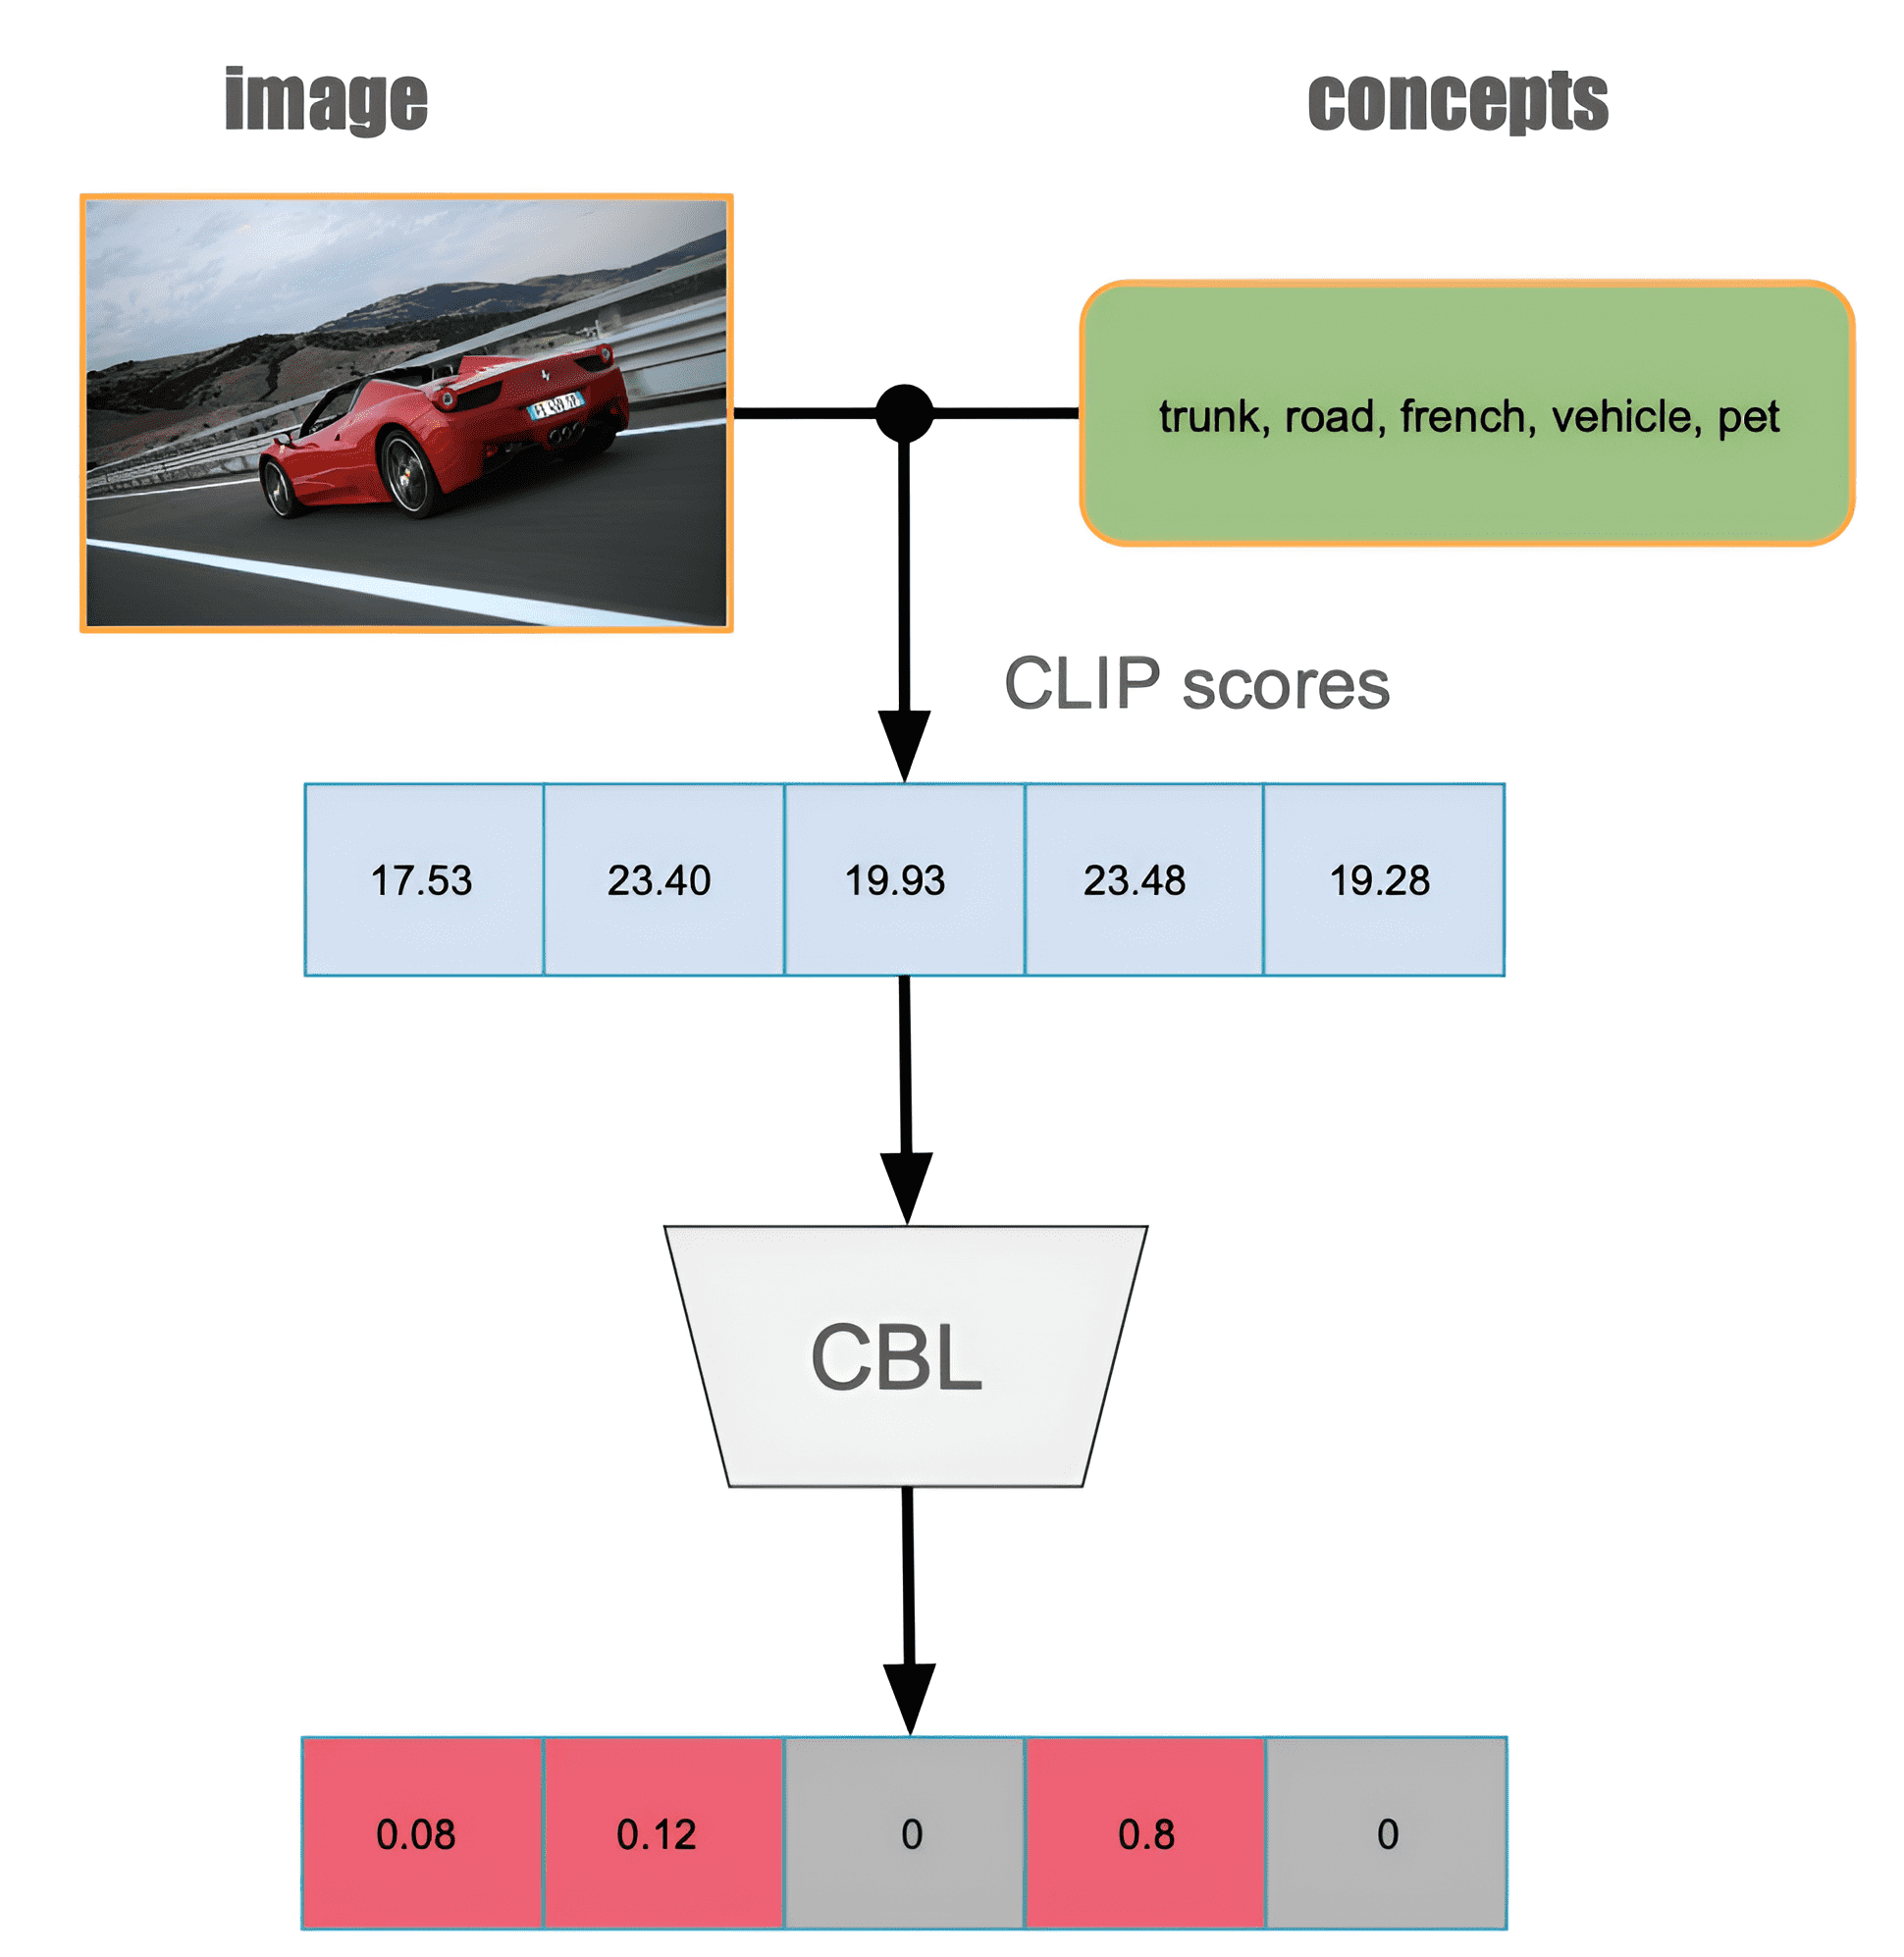
\includegraphics[width=0.6\columnwidth]{./figures/gumbel_example-compressed.png}}
\caption{Визуализация Sparse-CBM Concept Bottleneck слоев.}
\label{fig:gumbel_example}
\end{center}
\end{figure}
Если $\tau$ является обучаемым параметром (а не отжигается по фиксированному расписанию), эту схему можно интерпретировать как энтропийную регуляризацию \cite{szegedy2015rethinking,pereyra2017regularizing}. Высокоуровневое объяснение и вывод активаций Гумбеля можно посмотреть на \cite{alexandridis2022longtailed}.

\subsection{$\boldsymbol\ell_1$-CBM}
\label{sec:ellcbm}

Мы также обучаем концепт Bottleneck с помощью $\ell_1$-функции потерь. Ранее \cite{yuksekgonul2023posthoc} предлагал использовать штраф эластичной сети, а \cite{oikarinen2023labelfree} - среднее взвешенное между нормой Фробениуса и нормой матрицы элементов. Вместо этого мы показываем многообещающий результат только при использовании штрафа $\ell_1$. Штраф $\ell_1$ демонстрирует способность к спарсированию обучаемых слоев: оптимизатор пытается минимизировать потери, уменьшая веса, которые имеют ненулевой градиент, что приводит к тому, что некоторые веса устанавливаются точно в ноль, что эффективно удаляет соответствующие признаки из выходных данных CBL.

Начнем с определения следующей оптимизационной задачи:
\[
\min \limits_{W_{\mathrm{CBL}}} \mathop{\mathbb{E}}\limits_{(x, t, l)\sim\mathcal{D}}\big[\mathcal{L}_{\mathrm{CE}}(W_{\mathrm{F}}W_{\mathrm{CBL}}\psi(x, t), l) + \frac{\lambda}{|\mathrm{D}|}\Omega(W_{\mathrm{CBL}}) \big]_,
\]\label{eq:l1probl}где $\Omega(W_{\mathrm{CBL}})$ соответсвует регуляризатору. Мы используем:
\[
\Omega(W_{\mathrm{CBL}}) = \|W_{\mathrm{CBL}}\|_1
\] 
с единтвенной параметризацией $\lambda$. 
\section{Эксперименты}\label{sec:exps}

\paragraph{Бейслайн.} Здесь мы приводим основные сведения о моделях и алгоритмах, с которыми мы сравниваем нашу.

1) Мы оцениваем эффективность описанного фреймворка (раздел \ref{sec: framework}), в частности, Sparse-, Contrastive-, $\ell_1$-CBMs, сравнивая его с предыдущими Label-free \cite{oikarinen2023labelfree}, Post-hoc CBM \cite{yuksekgonul2023posthoc}, LaBo \cite{yang2023language} фреймворки на одних и тех же наборах данных \cite{5206848,wah_branson_welinder_perona_belongie_2011,krizhevsky2009learning,7968387}, но с разными базовыми моделями: в то время как в экспериментах с фреймворком Label-free, проведенных с ResNet50 \cite{he2015deep} и CLIP(ResNet50)\cite{radford2021learning}, мы используем только варианты архитектуры CLIP в качестве основы. Заметим, что оба фреймворка получают довольно схожие концепции, поскольку Label-free также включает опцию генерации концепций с помощью ConceptNet API. Также модель Label-free обучается двумя алгоритмами последовательно: сначала обучается CBLs с cos-cubed сходством, введенным в \cite{oikarinen2023labelfree}, затем последний FC-слой обучается с помощью решателя GLM-SAGA \cite{pmlr-v139-wong21b}. Мы также приводим сравнение с линейным зондированием, когда один линейный слой после CLIP обучается классификации. Подробное объяснение эксперимента с зондированием мы приводим в \cref{sec:appendix}.

2) Мы оцениваем эффективность описанного алгоритма Concept Matrix Search (раздел \ref{sec:cms}), сравнивая его с предыдущей работой Visual Classification via Description, которую мы обозначаем как метод "DescriptionCLS" в \cref{tab:cbms_tab}. Оба метода схожи в том, что они способны различать классы, выбирая тот, который имеет наивысший балл, предоставляемый некоторым \textit{rule}, и оба они не обучают никакую модель и используют только эмпирические формулы для предсказания целей более интерпретируемым способом. Наш \textit{rule} - это CMS (см. \cref{Alg:CMS}), в то время как метод "DescriptionCLS" опирается на функцию, которая дает оценку классу на основе того, сколько концептов этого класса чувствительны к изображению этого самого класса. Чувствительность понятия измеряется как логарифмическая вероятность того, что понятие относится к изображению в соответствии с косинусным сходством. CMS также использует эту меру, но она не создает прямого отображения класс-концепт, вместо этого мы проводим классификацию в более общем виде, учитывая только партию изображений и все концепции с классами. Кроме того, Concept Matrix Search играет роль более общего классификатора, и мы сравним их ниже, что весьма информативно, поскольку оба метода используют одну и ту же модель CLIP в качестве основы. Кроме того, необходимо привести сравнение с классификацией изображений с нулевым снимком. В этом случае мы рассматриваем пакет изображений и названия классов как входные данные для кодирования CLIP, который, в свою очередь, выдает матрицу "изображение - класс". Выполнив операцию argmax, мы определяем наиболее близкий класс.

\setcounter{table}{1}
\begin{table*}[t]
\caption{Сравнение перформанса Bottleneck моделей на основных датасетах. Мы наблюдаем превосходство Sparse-CBM над другими архитектурами на CIFAR10, CIFAR100 и CUB200 датасетах.}
\label{tab:cbms_tab}
\begin{center}
\begin{small}
\begin{sc}
\begin{tabular}{lccccr}
\toprule
Model & CIFAR10 & CIFAR100 & ImageNet & CUB200 & Places365 \\
\midrule
Sparse-CBM (Ours)    & \textbf{91.17\%} & \textbf{74.88\%} & 71.61\% & \textbf{80.02\%} & 41.34\% \\
$\ell_1$-CBM (Ours) & 85.11\% & 73.24\% & 71.02\% & 74.91\% & 40.87\%\\
Contrastive-CBM (Ours)   & 84.75\% & 68.46\% & 70.22\% & 67.04\% & 40.22\% \\
Label-free CBM    & 86.40\% & 65.13\% & \textbf{71.95\%} & 74.31\% & \textbf{43.68\%}    \\
Post-hoc CBM (CLIP)   &  83.34\%       &   57.20\%      &     62.57\%         &   63.92\%      &       39.66\%        \\
LaBo (full-supervised)             & 87.90\%&       69.10\%    &    70.40\%     & 71.80\% & 39.43\%
\\
\hline
Linear Probing             & 96.12\%&       80.03\%     &    83.90\%     & 79.29\% & 48.33\%     \\
\bottomrule
\end{tabular}
\end{sc}
\end{small}
\end{center}
\end{table*}
\begin{table*}[t]
\caption{Сравнение CMS и "DescriptionCLS"  на основных датасетах.}
\label{tab:cms_tab}
\begin{center}
\begin{small}
\begin{sc}
\begin{tabular}{lccccr}
\toprule
Method & CIFAR10 & CIFAR100 & ImageNet & CUB200 & Places365 \\
\midrule
CMS (Ours)    & \textbf{85.03\%} & 62.95\% & \textbf{77.82\%} & \textbf{65.17\%} & 39.43\% \\
DescriptionCLS  &    81.61\%     &      \textbf{68.32\%}    &     75.00\%     &   63.46\%    &   40.55\%    \\
Zero-shot  &    81.79\%     &      52.84\%    &     76.20\%     &   62.63\%    &   \textbf{41.12\%}    \\
\bottomrule
\end{tabular}
\end{sc}
\end{small}
\end{center}
\end{table*}

\subsection{CBM эксперименты}
\label{sec:cbmexp}

\paragraph{Набор концептов.} Мы сгенерировали большие наборы: один с 6 500 концептами, используя Llama-2, и второй с 5 000 концептами, используя ConceptNet \cite{article} API, и обработали их с помощью трансформатора предложений 'all-mpnet-base-v2', чтобы найти отсечения сходства, упомянутые в \textbf{шаг 2} (см. \cref{sec:framework}). API и обработали их с помощью трансформатора предложений 'all-mpnet-base-v2', чтобы найти отсечки сходства, упомянутые в \textbf{Шаг 2} (см. \cref{sec:framework}). Для самого большого набора мы подготовили все метки классов, чтобы создать из них концепты. Более того, для каждого набора данных в \cref{tab:concepts_size} также представлен соответствующий набор концептов. Мы называем самый большой набор концептов "Все концепты", который можно увидеть в \cref{fig:cms_acc}. Каждый набор данных имеет свой собственный набор концептов, сгенерированный из классов набора данных в соответствии с \textbf{шаг 2}. Для корректного сравнения, представленные в \cref{tab:cbms_tab} модели были обучены \textit{only} с концептами, сгенерированными ConceptNet.

\paragraph{Модели.} CLIP-ViT-L/14 и B/32\footnote{Упомянутую модель CLIP-ViT-B/32 можно найти на хабе Hugging Face \texttt{https://huggingface.co/openai/clip-vit-base-patch32}} в качестве основы для всех CBM-экспериментов. В зависимости от набора данных, размер этих моделей варьируется. Самая маленькая конфигурация B/32
\begin{figure}%{0.285\textwidth}
\setcounter{table}{0}
\captionof{table}{Зависимость размера набора концептов от набора данных.}
\label{tab:concepts_size}
\begin{center}
\begin{small}
\begin{sc}
\begin{tabular}{lr}
\toprule
 Dataset & \# of concepts   \\
\midrule
CIFAR10  & 120   \\
CIFAR100 & 944 \\
ImageNet & 4,751 \\
CUB200 & 926 \\
Places365 & 2,900\\
"All concepts" & 5,051 \\
\bottomrule
\end{tabular}
\end{sc}
\end{small}
\end{center}
\end{figure}
 для CIFAR10 имеет размер 151,3 млн параметров и 50 000 обучаемых параметров, что эквивалентно 0,6 ГБ. Самая большая - L/14 для ImageNet-1K: 455 миллионов параметров; 27,3 миллиона обучаемых параметров и размер 1,81 ГБ. Для наглядности мы показываем точную информацию в \cref{tab:backbone_nets} (до обучения). А в \cref{tab:cbms_tab} мы приводим результаты для конфигурации CLIP-ViT-L/14.

\paragraph{Оборудование.}
Мы обучали наши модели на одной машине с 4 графическими процессорами NVIDIA A100-SXM4-80GB и A100-PCIE-40GB, по два каждого типа. Для наших конфигураций МД каждый шаг обучения со скоростью обучения по умолчанию, указанной в таблицах \ref{tab:backbone_nets}, \ref{tab:concepts_size} данных, занял менее 1 секунды для конфигурации CLIP-ViT-B/32 backbone и немного больше для CLIP-ViT-L/14. Мы обучили каждую из моделей Sparse, $\ell_1$, Contrastive-CBM на ImageNet-1K \cite{russakovsky2015imagenet} за 20 000 шагов, что заняло чуть больше 5,5 часов для каждой модели (см. \cref{fig:curves}). Наши реализации не зависят от конкретных аппаратных архитектур.

\begin{figure}[t]
\begin{center}
\centerline{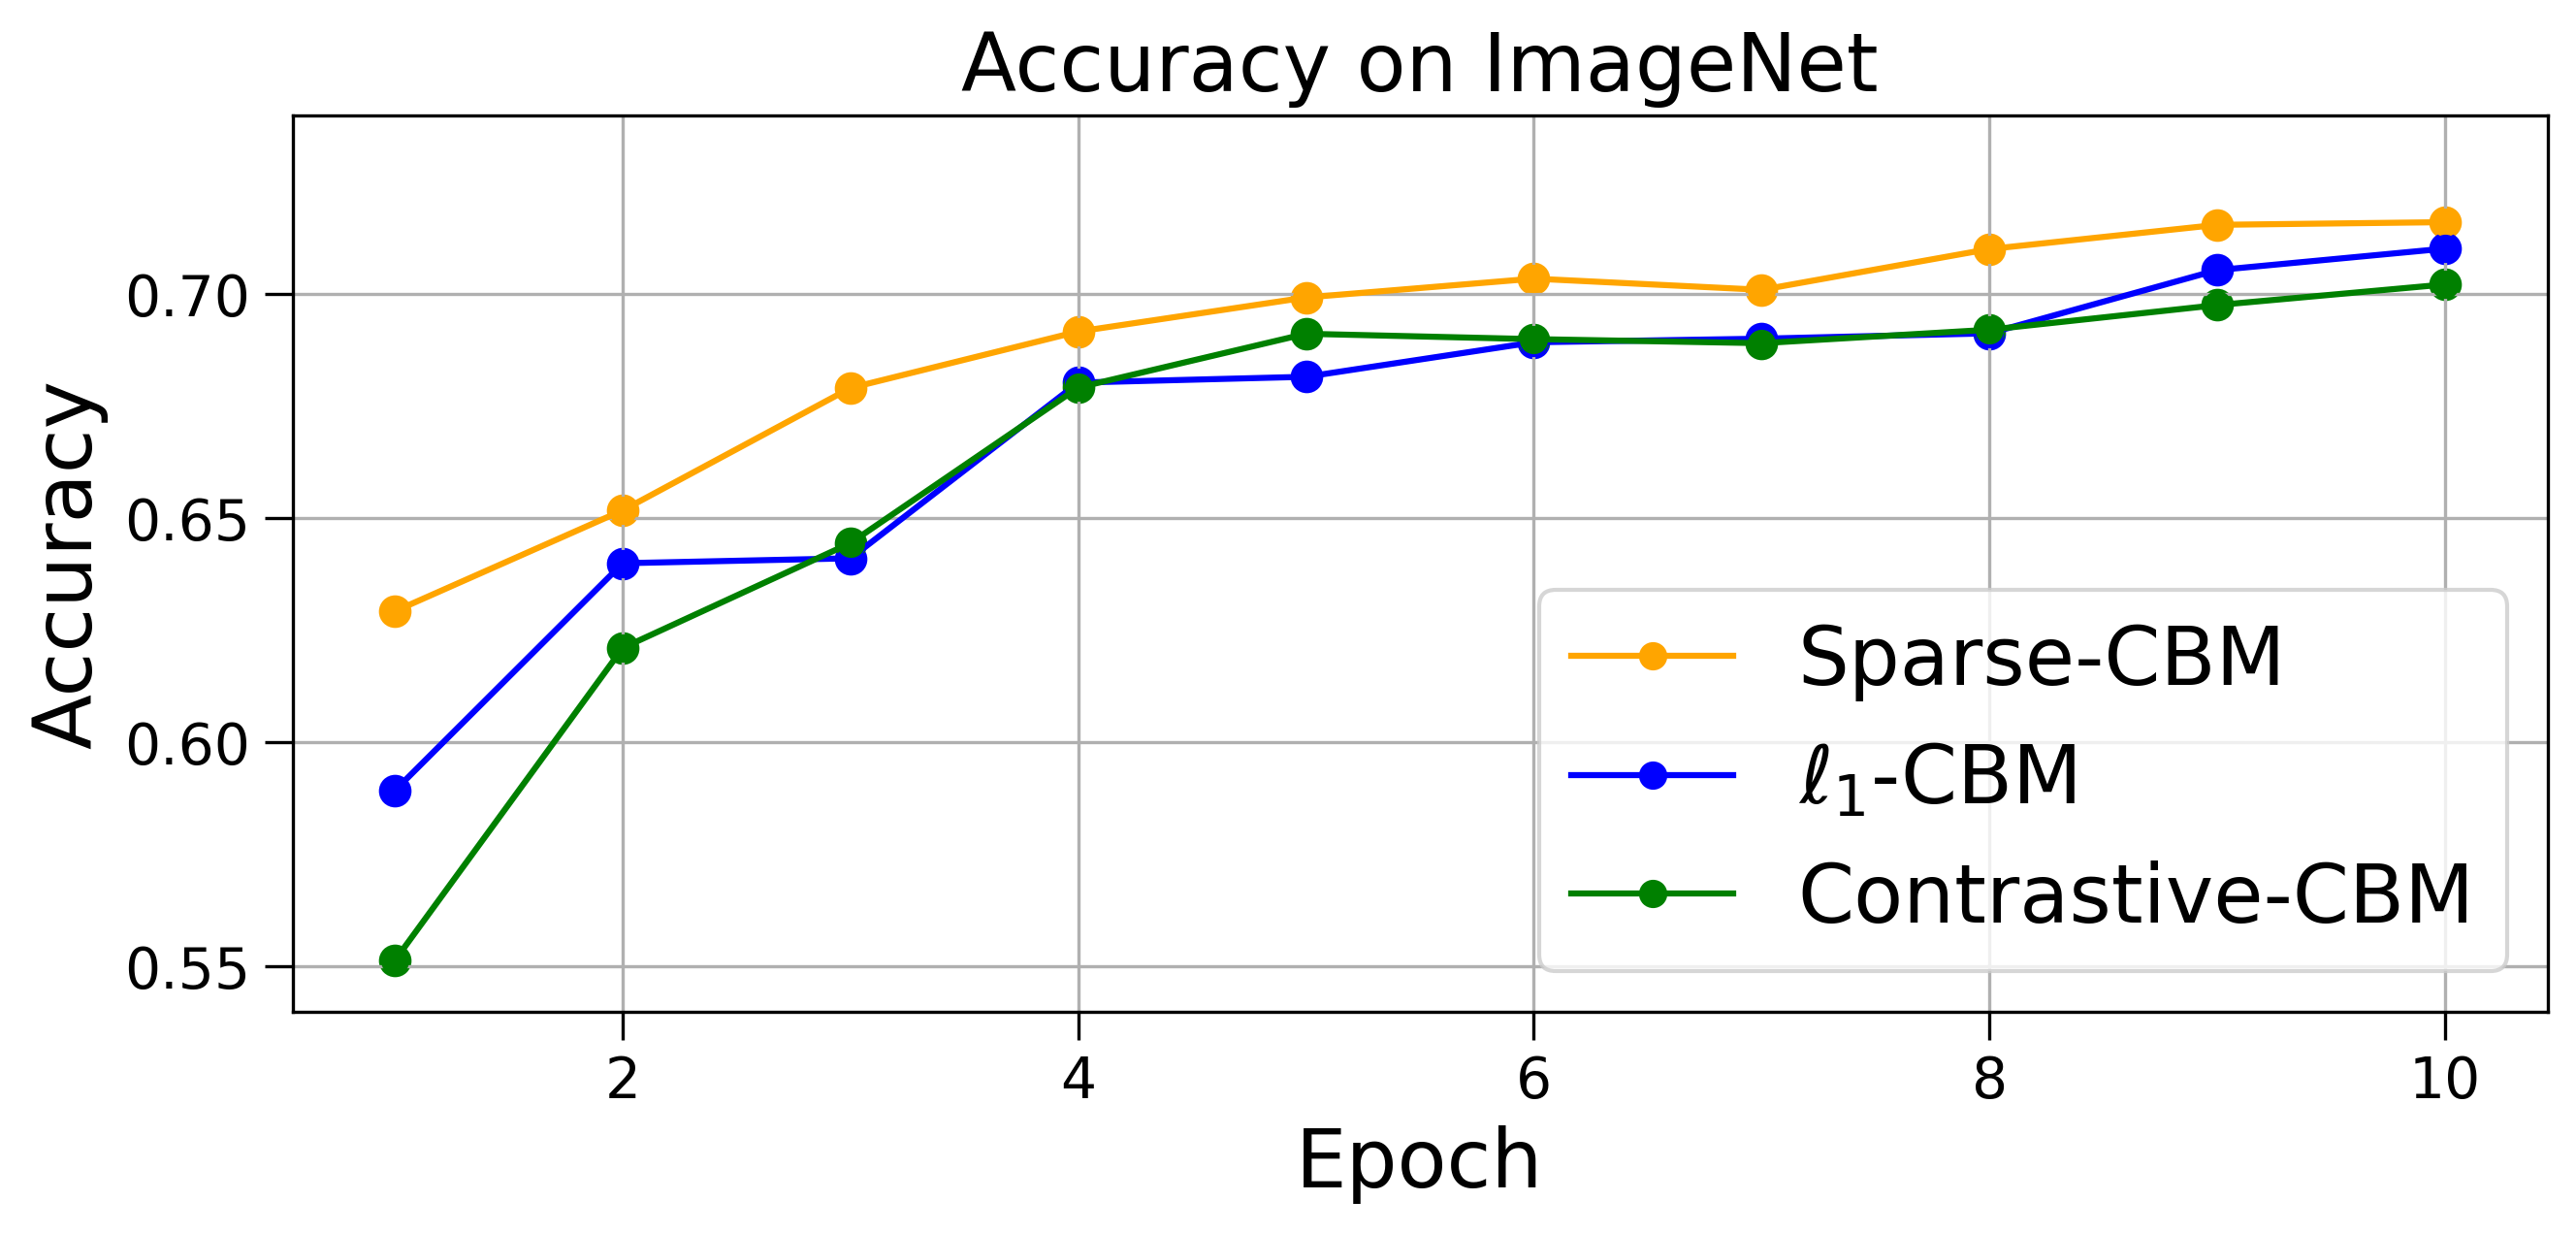
\includegraphics[width=\columnwidth]{./figures/cbms_acc_imnet.png}}
\caption{Сравнение CBM мотодов на валидационной подвыборке датасета ImageNet.}
\label{fig:cbm_acc}
\end{center}
\vskip -0.45in
\end{figure}
\paragraph{Рабочая нагрузка}. Мы поддерживаем схему \textit{последовательных узких мест} из \cite{koh2020concept}. Действительно, сначала мы производим градиентное обновление весов $W_{\mathrm{F}}$ и $W_{\mathrm{CBL}}$ с учетом их параметров независимо друг от друга, а затем, во время следующего прохода вперед, FC получает на вход логиты из обновленного CBL. Таким образом, после каждой итерации задач минимизации CBL и FC для классификатора создается новое представление концепта.

\subsection{CMS эксперименты}
\label{sec:cmsexp}

В этом разделе мы сравним два алгоритма: наш CMS \ref{Alg:CMS} и основной метод, предложенный в \cite{menon2022visual}. Оба они используют базовые возможности модели CLIP. Мы тестируем их на одной и той же конфигурации CLIP-ViT-L/14. Мы показали превосходство нашего метода на нескольких наборах данных, которые можно увидеть в \cref{tab:cms_tab}. Авторы \cite{kazmierczak2023clipqda} измерили зависимость точности при обнулении определенного количества концептов, а \cite{chauhan2023interactive} исследовали влияние нескольких относительных концептов. Мы же измерили зависимость точности от различных наборов понятий: почти синонимов (сходство "понятие-класс" 0,95 вместо 0,85), сгенерированных ConceptNet как обычно, одного набора многих понятий (большинство из них бесполезны для данных CIFAR10) и 3 000 случайно сгенерированных слов. Результаты представлены в \cref{fig:cms_acc}.
\section{Обсуждение}\label{sec:disc}

\cref{tab:cbms_tab} демонстрирует превосходство Sparse-CBM по сравнению с Label-free на всех наборах данных, кроме ImageNet и Places365. Более того, Contrastive-CBM имеет самый низкий общий балл. Мы интерпретируем эти наблюдения следующим образом:

\begin{figure}[t]
\begin{center}
\centerline{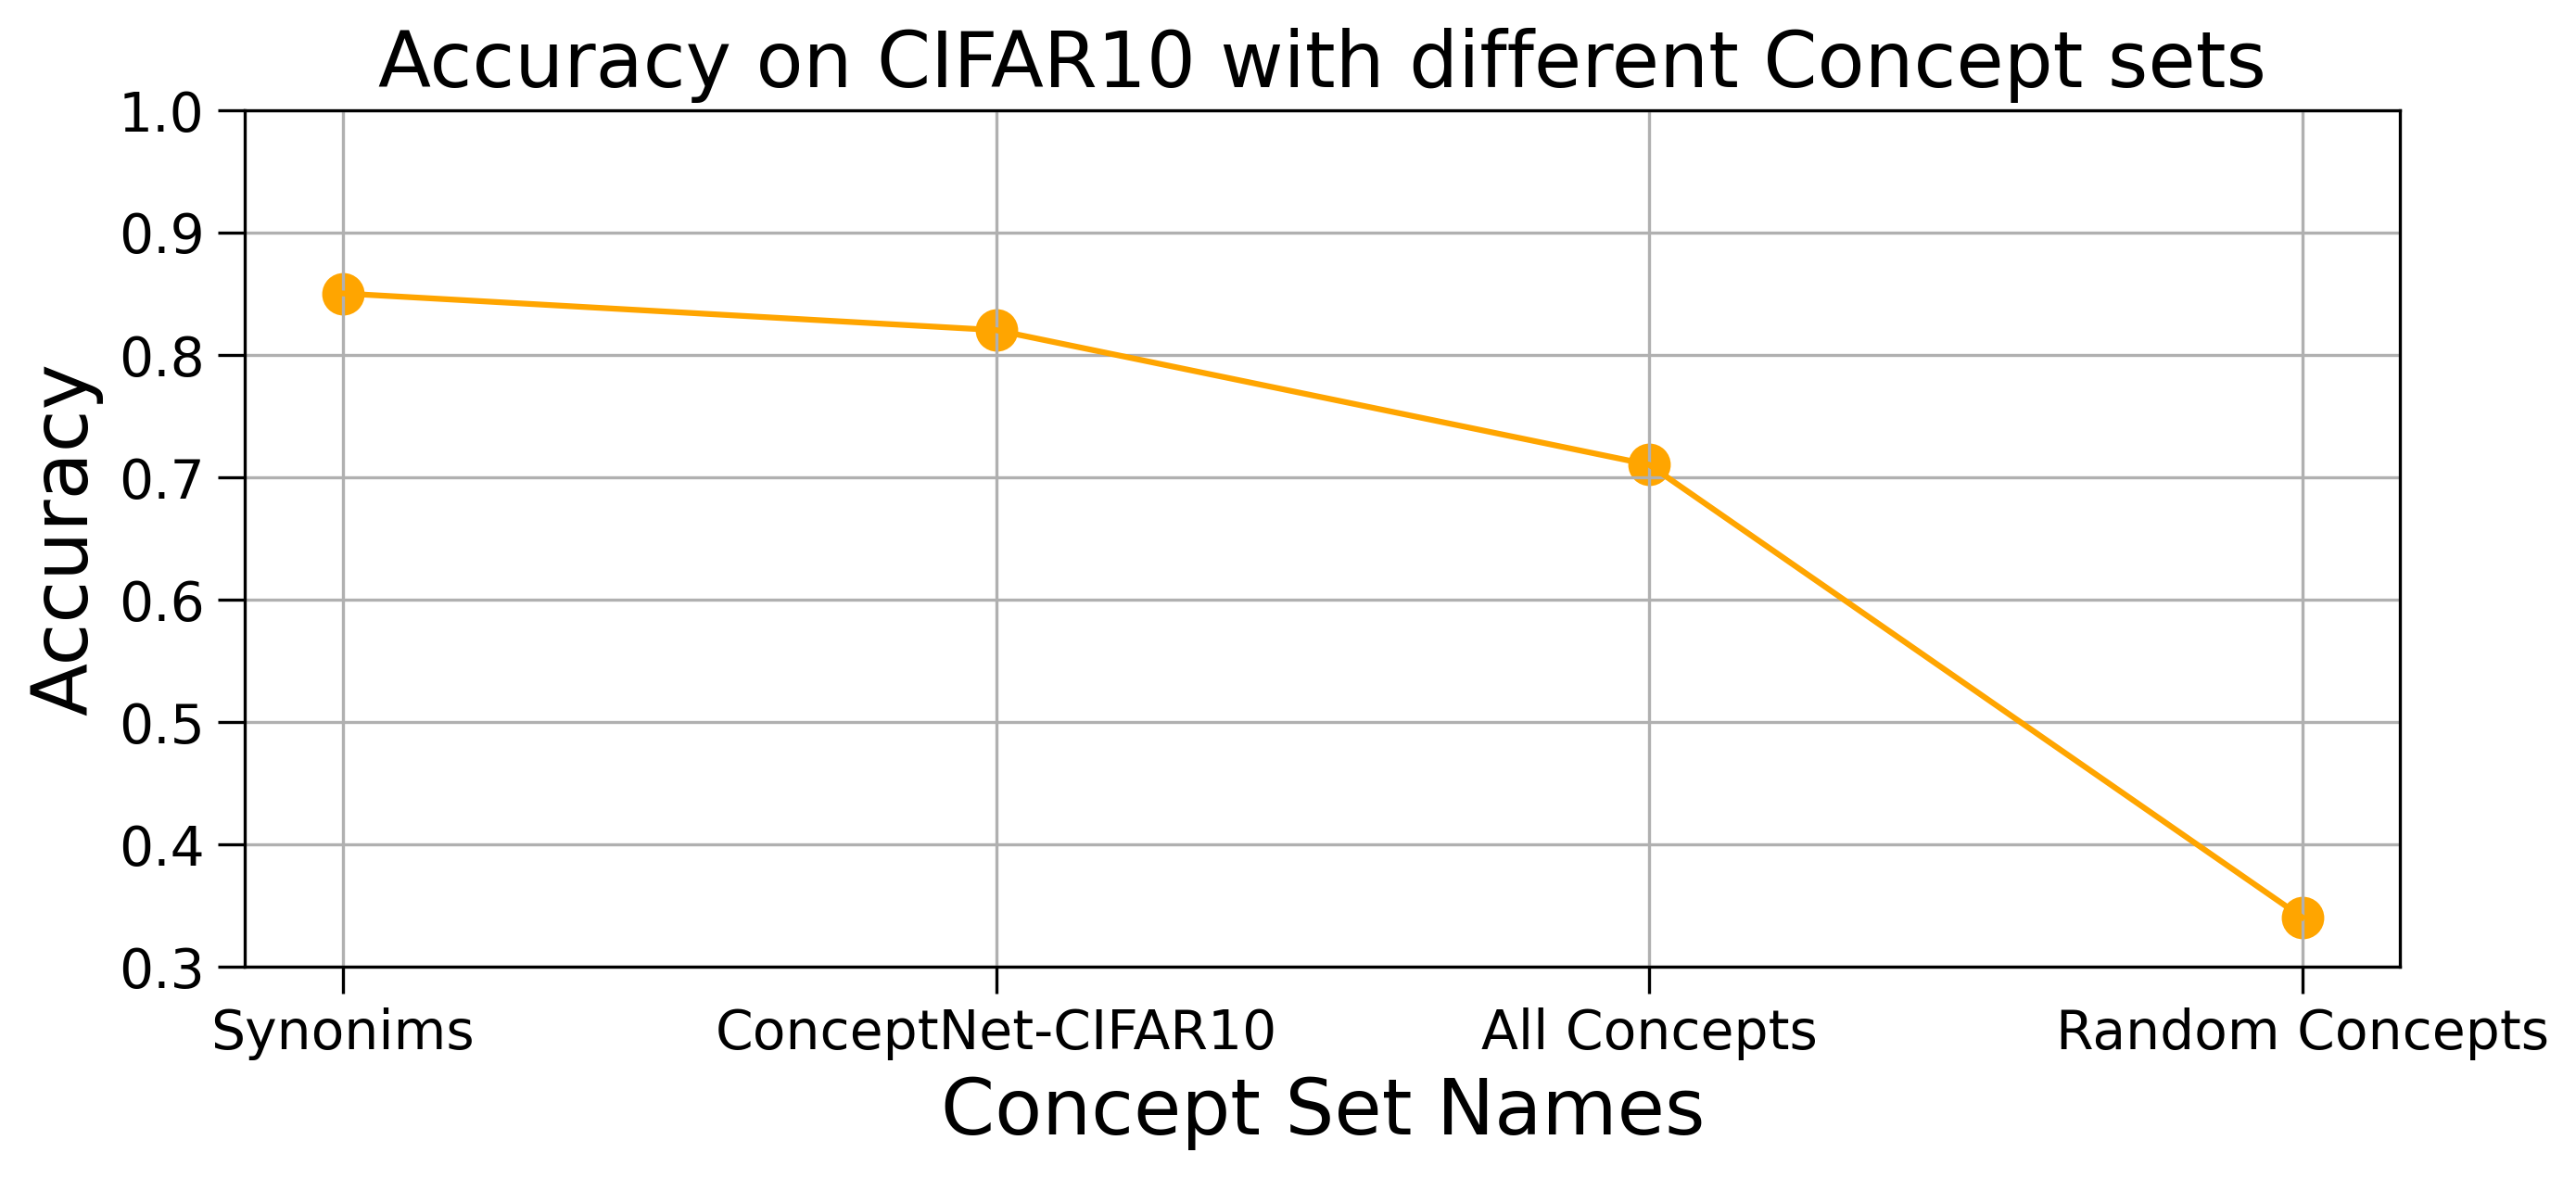
\includegraphics[width=\columnwidth]{./figures/cms_acc_cifar10.png}}
\caption{Зависимость качества CMS от набора конйептов.}
\label{fig:cms_acc}
\end{center}
\end{figure}



1) Из-за \cref{tab:concepts_size} пропорция между размером CBL и размером FC различается. В то время как такие наборы данных, как CIFAR10 и CIFAR100, содержат в $\approx$ 10 раз больше концептов, чем классов, для ImageNet и Places365 это число, а значит и пропорция между размерами слоев, примерно в 4,6-4,7 раза больше. Мы настаиваем на том, что разреженность внутренних слоев приносит больше пользы при увеличении размерности CBL по сравнению с размерностью выхода последнего полностью связанного слоя.

2) Методу Contrastive-CBM не хватает интерпретируемости представления концептов, т. е. разреженности CBL (подробное сравнение интерпретируемости см. в \cref{sec:concepts_interpretability}).

Мы также ссылаемся на алгоритм CMS и показываем снижение точности в зависимости от "качества" концептов, что делает наш метод и подобные ему менее универсальными. С другой стороны, при "хорошем" наборе понятий для каждого набора данных мы показываем, что CMS превосходит Zero-shot CLIP. Это говорит о том, что модель получает дополнительную "уверенность" при предсказании не только наиболее похожего класса, но и при получении нескольких значимых концептов на изображение.

\subsection{Исследование абляции}\label{sec:abl}
Компоненты, введенные в наш фреймворк, приводят к снижению итоговой производительности по сравнению с линейным зондированием (см. \cref{tab:cbms_tab}), обеспечивая при этом интерпретируемость, которую мы представляем в \cref{sec:concepts_interpretability}. Наш метод и его интуиция, заключающаяся в том, чтобы сделать внутреннее представление более разреженным, понятны, и он оказывается перспективным для извлечения значимых понятий. Тем не менее, "жесткая" (т.е. делающая выборки непосредственно одномоментными) выборка в контрастном Gumbel-Softmax loss скорее вредит производительности Sparse-CBM, чем улучшает ее. В то же время Contrastive-CBM выполняет двойной softmax на CBL, который обеспечивает отсутствие разреженности и достигает худшего результата по точности, что опять же подтверждает нашу гипотезу о полезности разреженных внутренних представлений. И фреймворк CBM, и метод CMS полагаются на сгенерированный набор концептов. С концептами, которые лучше приспособлены к набору данных, мы показываем более высокие результаты по точности классификации, с другой стороны, мы хотим, чтобы концепты были более разнообразными, что эмпирически определено в \cref{sec:framework} и в предыдущей \cite{oikarinen2023labelfree} работе, тогда нам не принципиально менять количество концептов вручную, мы предпочтем сохранить сгенерированные.

\subsection{Ограничения}\label{sec:lims}

Помимо достигнутых показателей точности, мы сообщаем об основных ограничениях нашего фреймворка и алгоритма \ref{Alg:CMS}. LLM, предложенный во фреймворке CBM, по-прежнему не влияет на процесс классификации, то есть не поддерживает генерацию концептов во времени и работает только на \textbf{шаге 2}. Оба варианта CMS и CBM не модифицируют латентное пространство CLIP, что делает наш подход менее универсальным. Хотя мы вносим вклад в понимание разреженных CBL, эффективность моделей узких мест с также разреженными FC все еще не раскрыта. То же самое относится и к проблеме сквозного редактирования концепт-блотлека (см. \cref{sec:bottls}). Наконец, метод CMS может быть полезен в качестве дополнения к CLIP, но в долгосрочной перспективе не может конкурировать с подходами МД из-за ситуации, показанной в \cref{fig:cms_acc}.   
\nocite{JMLR:v9:vandermaaten08a}

\bibliography{ref}
\newpage

\appendix
\section{Аппендикс}
\label{sec:appendix}

Мы сравниваем наши архитектуры Sparse-, $\ell_1$-, Contrastive-CBM с Post-hoc CBM \cite{yuksekgonul2023posthoc} и LaBo \cite{yang2023language} с точки зрения точности в задаче классификации изображений. В то время как интерпретируемость концептов сравнивается со свойствами магистральной мультимодальной модели в \cref{sec:concepts_interpretability}. Поскольку фреймворки Post-hoc также позволяют создать модель Concept Bottleneck над стандартной, мы оцениваем этот метод на модели CLIP-ViT-L/14 для справедливого сравнения, в то же время архитектуры LaBo построены с той же самой базовой моделью с помощью defalut. Кроме того, мы приводим результаты для линейного зондирования CLIP-ViT-L/14. В этом случае мы добавляем только один линейный слой после матрицы Image-Class, возвращаемой CLIP. Обновленные результаты можно посмотреть в \cref{tab:cbms_tab}.

Настройка "full-supervised" в LaBo означает, что архитектура обучается на всех доступных изображениях. Мы отмечаем это в связи с тем, что рассматриваются режимы обучения \cite{yang2023language} zero-shot и N-shot.

\section{Дополнительные эксперименты}
В этом разделе мы сообщаем о дополнительных результатах оценки фреймворка CBM (раздел \ref{sec:framework}) и алгоритма CMS (раздел \ref{sec:cms}).

\subsection{Обучение Concept Bottleneck Model}
Мы приводим несколько графиков (\cref{fig:sparse_best_cifar,fig:sparse_best_cub,fig:sparse_best_imnet}), наблюдаемых во время обучения Sparse-CBM на CIFAR10, CUB200 и ImageNet-1K.

\begin{figure}[h] %ht!
\centering
   \begin{subfigure}%[b]%{3.5cm}
     \centering
    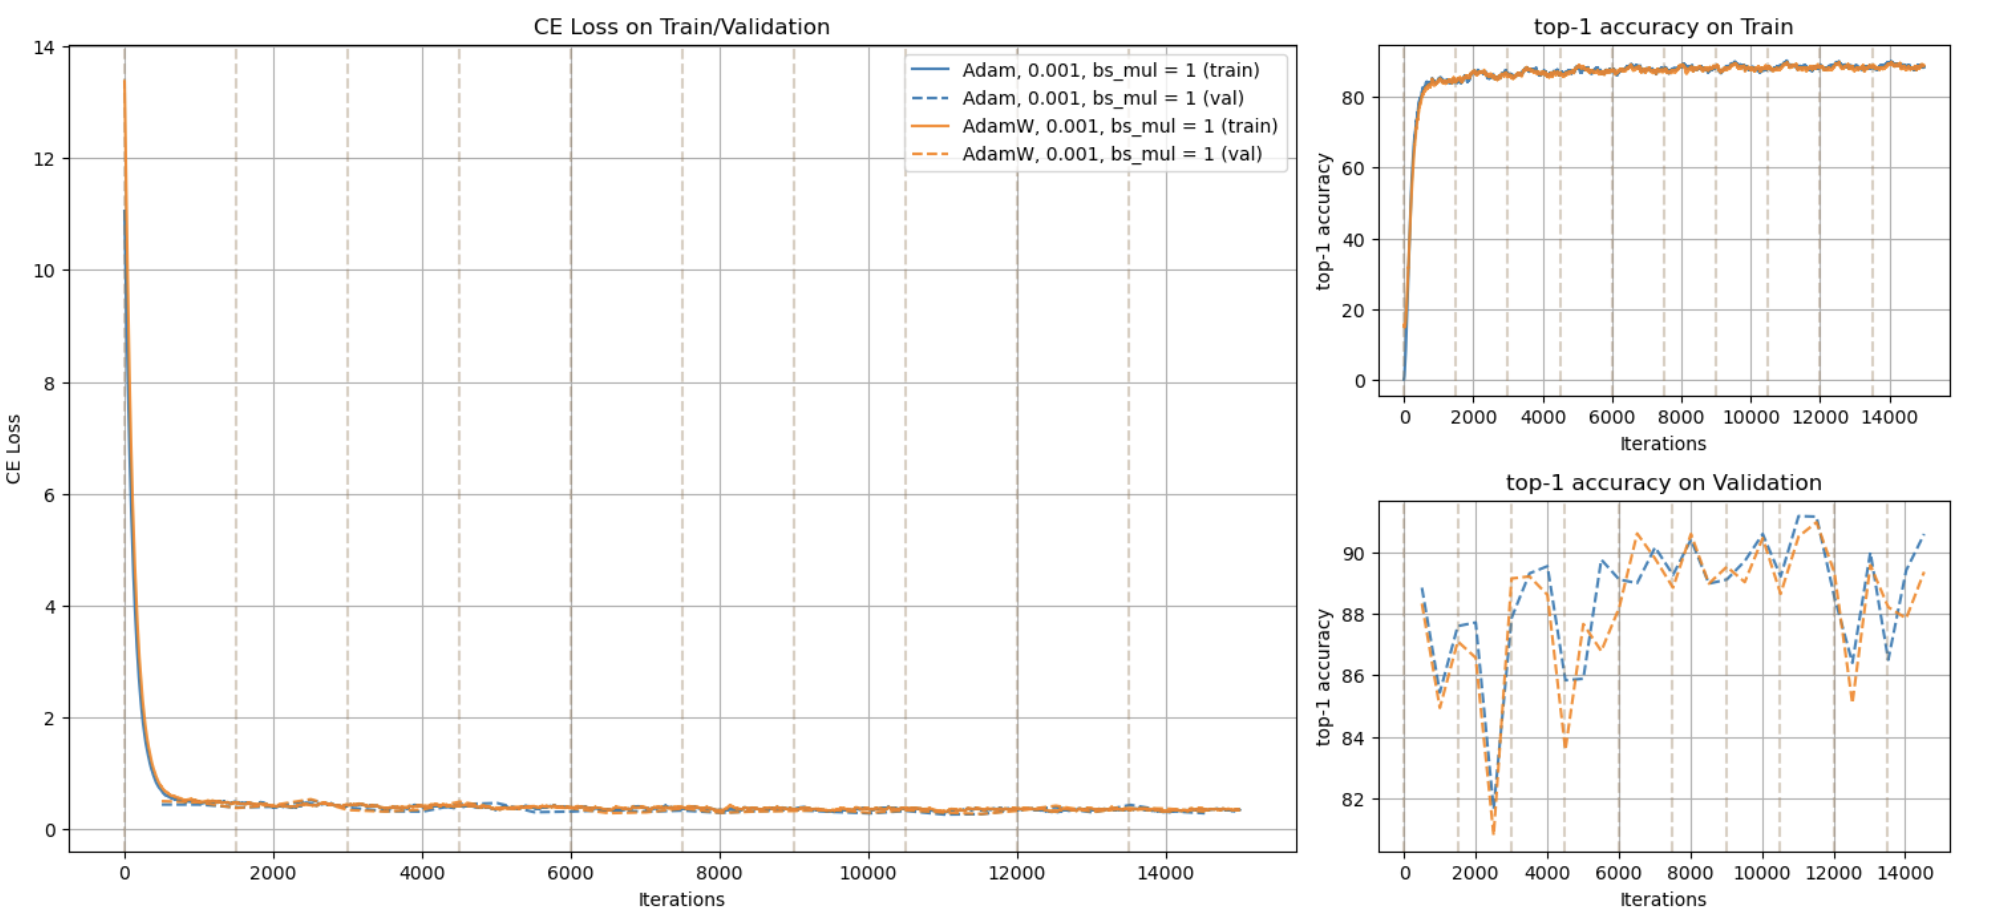
\includegraphics[width=0.5\linewidth]{./figures/sparse_cifar10_91.png}
    \caption{Лучший результат Sparse-CBM на CIFAR10.}
    \label{fig:sparse_best_cifar}
    \end{subfigure}
    \begin{subfigure}%[b]%{3.5cm}
    \centering
      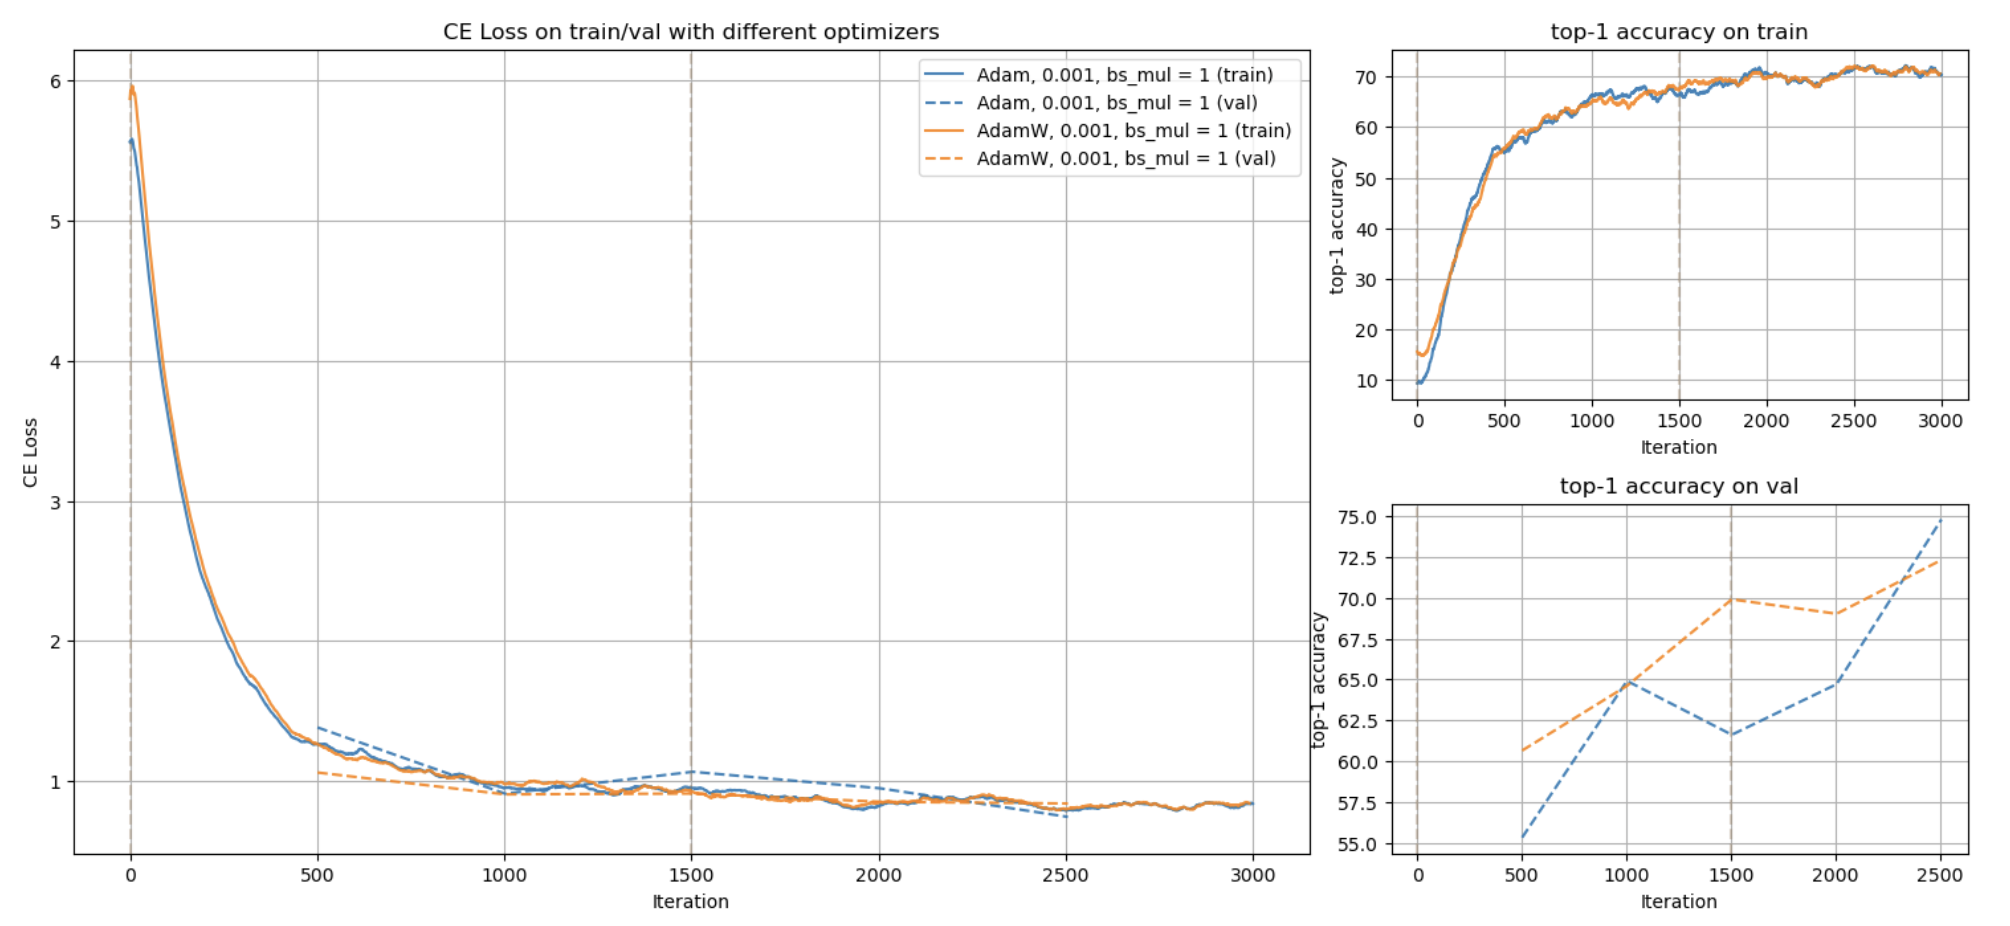
\includegraphics[width=0.5\linewidth]{./figures/sparse_imnet_71.png}
    \caption{Лучший результат Sparse-CBM на CUB200.}
    \label{fig:sparse_best_imnet}
    \end{subfigure}
    \begin{subfigure}%[b]%{3.5cm}
     \centering
  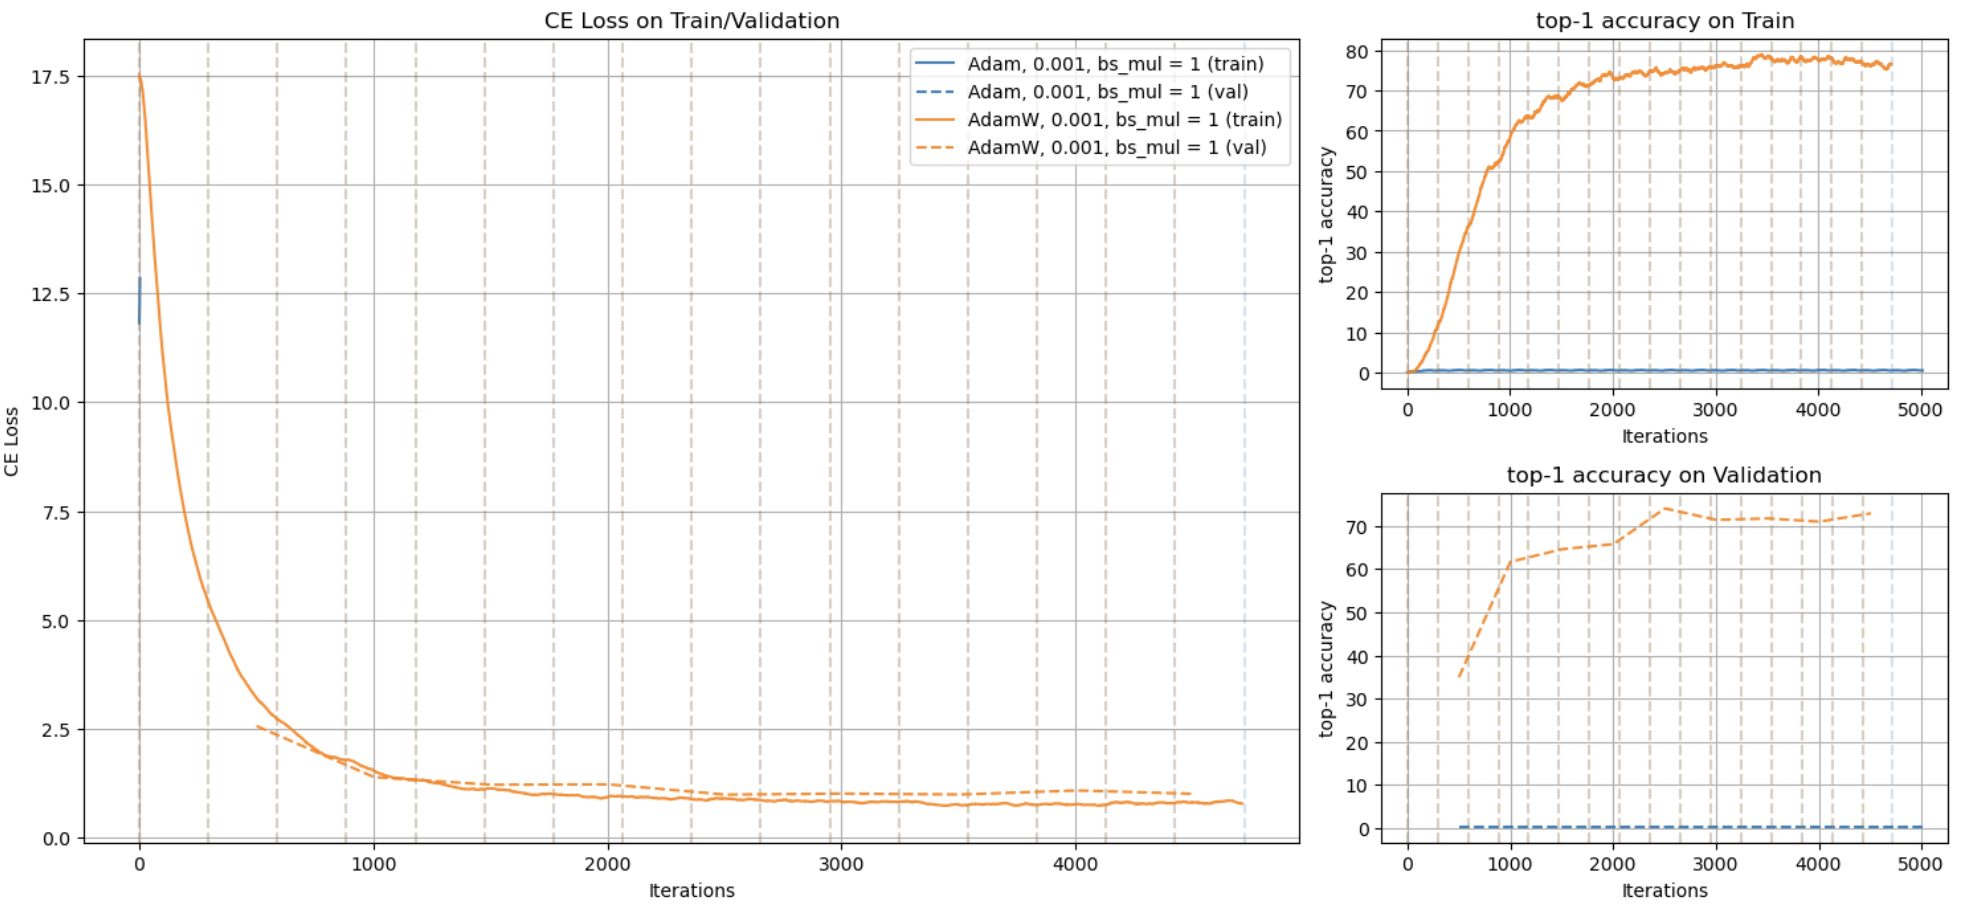
\includegraphics[width=0.5\linewidth]{./figures/sparse_cub_76.png}
    \caption{Лучший результат Sparse-CBM на ImageNet-1K.}
    \label{fig:sparse_best_cub}
    \end{subfigure}
    \caption{Обзор режима обучения с использованием разреженного CBM на нескольких наборах данных. Мы наблюдаем аналогичные кривые потерь при обучении на всех данных. Но для ImageNet обучение начинается с меньшей скорости обучения.}\label{fig:curves}
\end{figure}

\section{Дополнительные данные}

\begin{table}[h]
\caption{Конфигурации магистральных моделей. Пересечения указывают на размер модели с соответствующей конфигурацией.}
\label{tab:backbone_nets}
\begin{center}
\begin{small}
\begin{sc}
\begin{tabular}{lcccr}
\toprule
B/32 & L/14 & Dataset   \\
\midrule
 0.57GB & 1.63GB &  CIFAR10 \\
 0.58GB& 1.64GB & CIFAR100 \\
 0.68GB &  1.74GB & ImageNet \\
 0.58GB& 1.64GB & CUB200 \\
 0.61GB& 1.67GB & Places365 \\
\bottomrule
\end{tabular}
\end{sc}
\end{small}
\end{center}
\end{table}

\section{Визуализации}
\begin{figure}[ht]
\begin{center}
\centerline{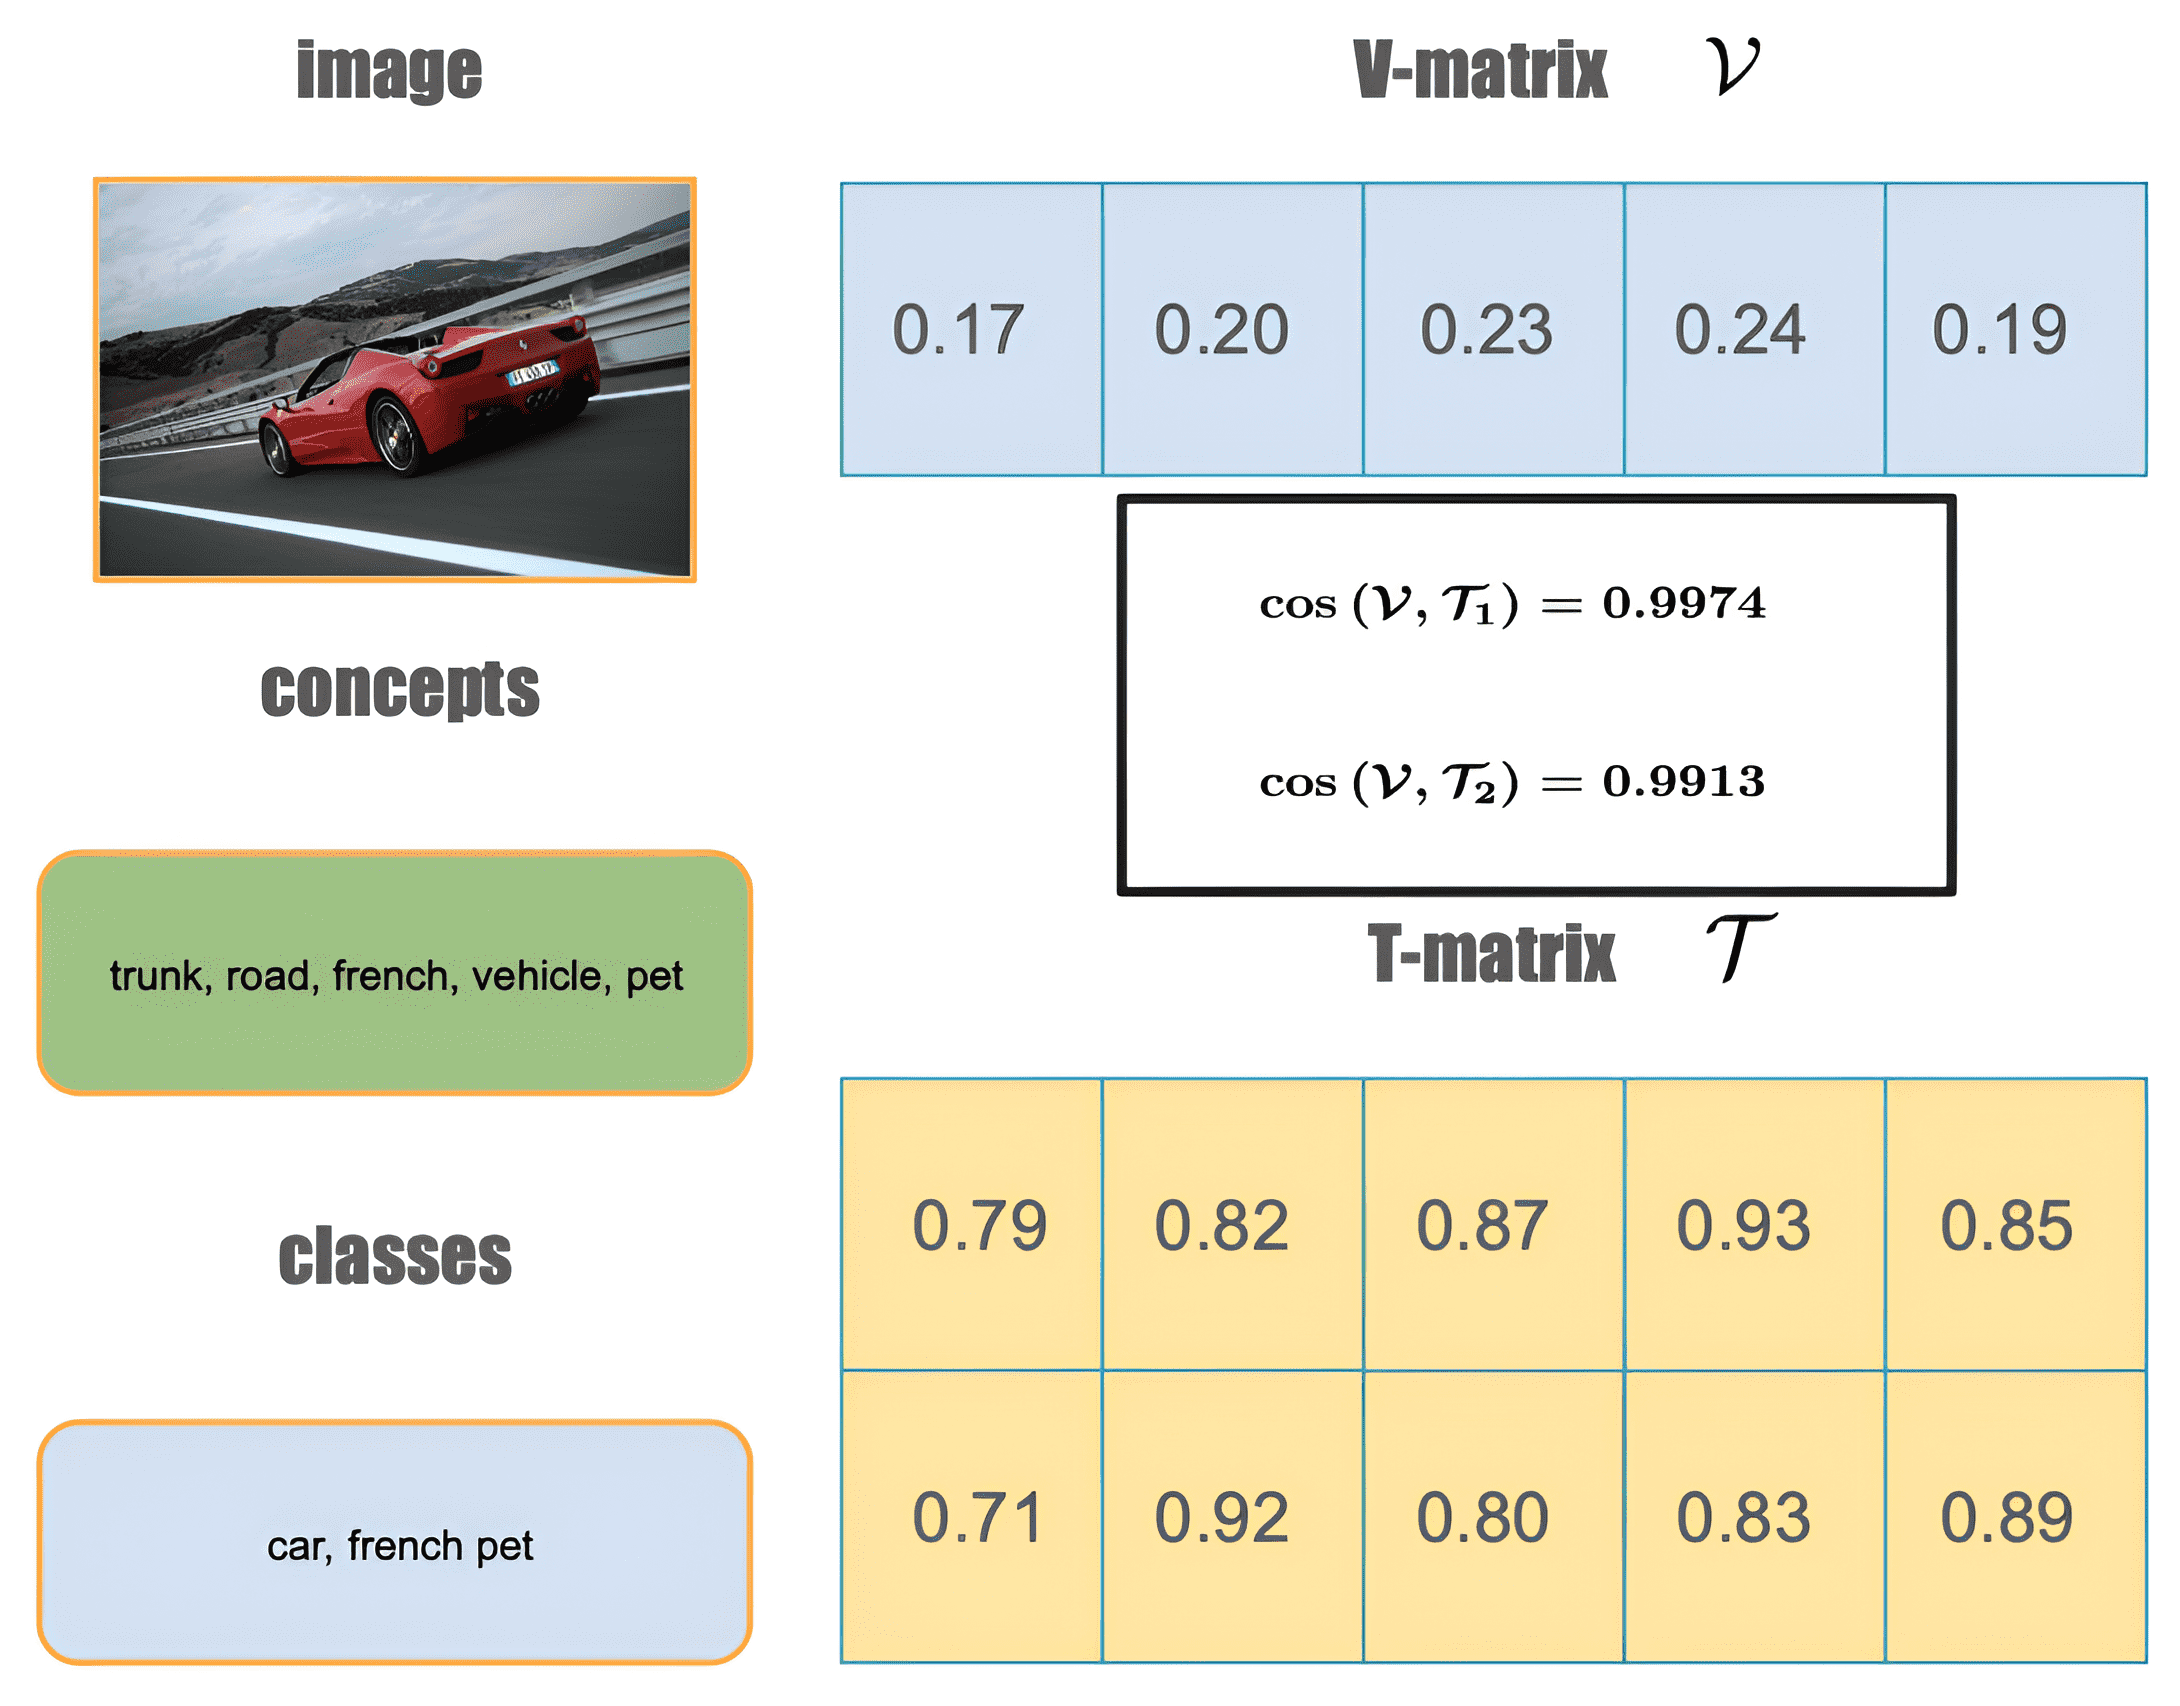
\includegraphics[width=0.5\columnwidth] {./figures/cms_example-compressed.png}} 
\caption{Визуализация Concept Matrix Search \textit{гипотезы} для простого случая 1 картинки, 5 концептов и 2 классов.}
\label{fig:cms_example}
\end{center}
\end{figure}

\subsection{Анализ латентного пространства CLIP}
В этом разделе мы представим дополнительные эксперименты с латентным пространством CLIP. Во-первых, используя CLIP, мы построили двумерную t-SNE карту вкраплений CIFAR10 вместе с их концептами и классами. Интересным результатом является то, что это пространство не просто разделено на два кластера: один соответствует текстовой модальности, а второй - визуальной, но и, если добавить проекцию случайных слов на t-SNE, мы наблюдаем ее пересечение с концептами. Соответствующий эксперимент представлен в \cref{fig:tsne}

С помощью метода кластеризации k-means мы строим различимые по CLIP кластеры (см. \cref{fig:kmeans}).

Важным моментом в t-SNE-визуализации является то, что латентное пространство CLIP-подобных моделей строго делится на два кластера: один соответствует вкраплениям изображений, а второй - текстовой модальности. Интуиция, лежащая в основе МД, подсказывает, что распределение модальностей должно полностью отличаться от того, что наблюдается в \cref{fig:tsne}. Действительно, для удобства интерпретации предполагается, что вкрапления изображений должны быть ближе к векторам соответствующих понятий и классов. Если это так, то простой алгоритм kNN сможет найти наиболее релевантные понятия, что в нашем случае неверно. Таким образом, мы выделяем нерешенную проблему построения моделей, которые будут изучать подобное латентное пространство сквозным образом.

\begin{figure}[h]
\begin{center}
\centerline{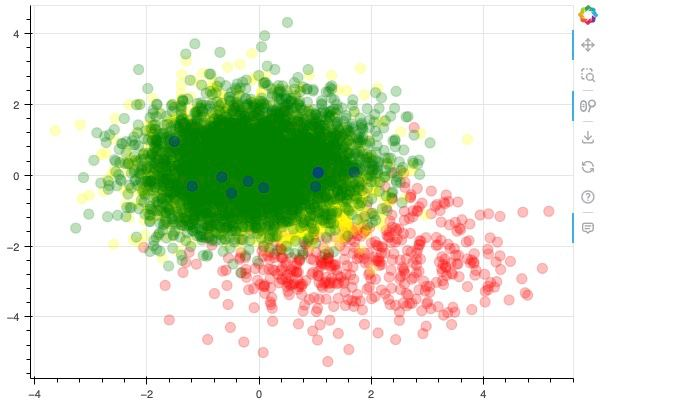
\includegraphics[width=0.5\columnwidth]{./figures/cifar10tsne.jpg}} 
\caption{Визуализация CIFAR10 t-SNE. Зеленые точки относятся к проекции понятий, синие - к классам, красные - к изображениям, а желтые - к случайным словам.}
\label{fig:tsne}
\end{center}
\end{figure}

\begin{figure}[t]%t
\begin{center}
\centerline{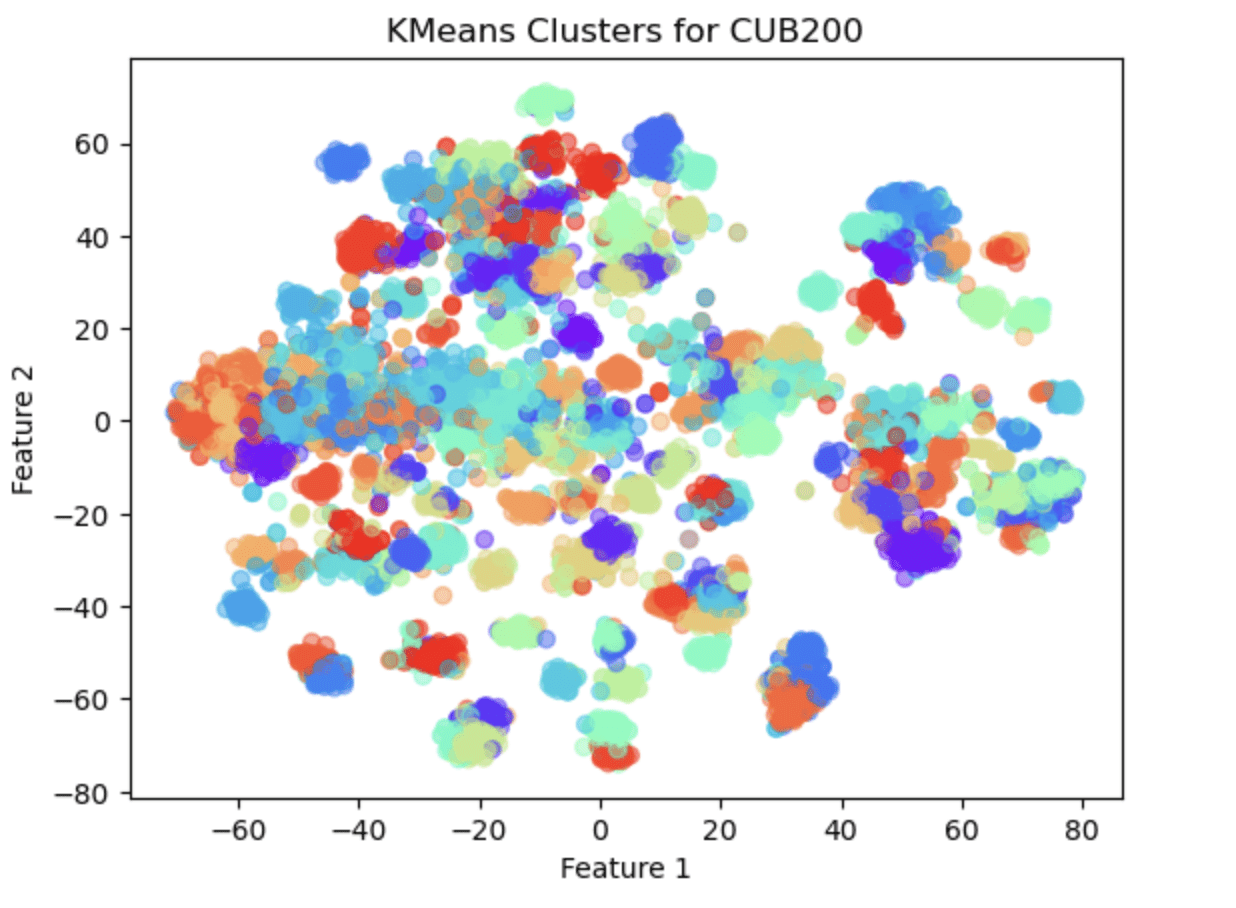
\includegraphics[width=\columnwidth]{./figures/cub_kmeans-compressed.png}} 
\caption{Визуализауия k-means кластеров эмбеддингов картинок из CUB200 полученных с помощью CLIP.}
\label{fig:kmeans}
\end{center}
\end{figure}


\subsection{Интерпретируемость концептов}
\label{sec:concepts_interpretability}
Мы сравниваем возможности интерпретации frawework с базовыми свойствами извлечения признаков CLIP на подмножествах изображений из наборов данных Places365, CUB200, CIFAR10 и ImageNet. Мы выбираем как базовые изображения для наглядности, так и сложные, с большим количеством внутренних деталей. Для CLIP-подобных моделей мы регистрируем топ-к (k=10) наивысших оценок точечного продукта, а для наших фреймворковых архитектур - результаты работы Concept Bottleneck Layer. Отметим, что дальнейшие результаты в \cref{fig:concepts_1,fig:concepts_2,fig:concepts_3,fig:concepts_4,fig:concepts_5,fig:concepts_6} проведены с использованием магистральной модели CLIP-ViT-L/14. Мы определенно наблюдаем распыление активаций с помощью как Sparse-, так и $\ell_1$-CBM. Также показано, что концептуальный слой Bottleneck Layer, обученный с контрастной целью, производит довольно схожие активации по сравнению с базовой моделью CLIP. В то же время итоговая точность становится выше при использовании разреженных и $\ell_1$-моделей, что говорит о превосходстве методов, разрежающих внутренние слои модели.

В данной работе мы не приводим интерпретируемые матрицы поиска концептов, поскольку этот подход к классификации с узкими местами концептов не модифицирует базовую модель CLIP, поэтому она обладает теми же свойствами, что и \cref{fig:concepts_1,fig:concepts_2,fig:concepts_3,fig:concepts_4,fig:concepts_5,fig:concepts_6} (a).
\begin{figure}[h] %ht!
\centering
   \begin{subfigure}%[b]%{3.5cm}
     \centering
    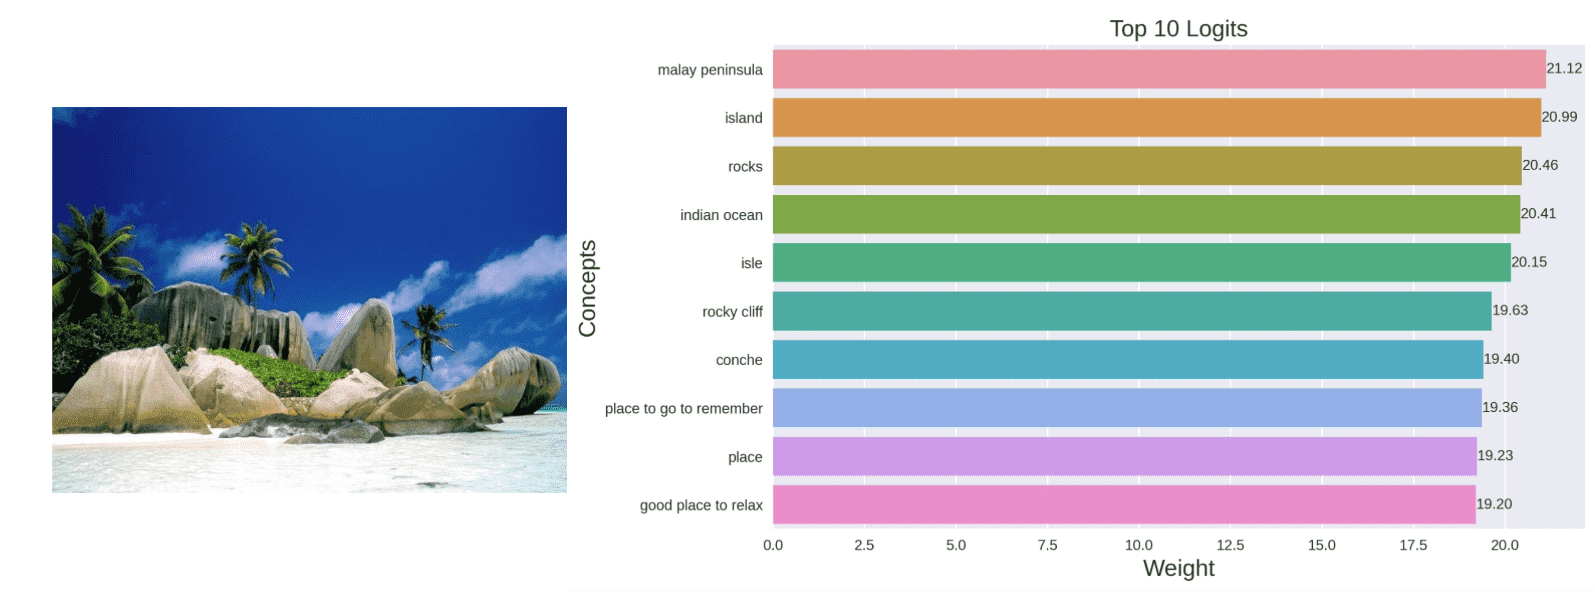
\includegraphics[width=0.75\linewidth]{./figures/clip_im_1-compressed.png}
    % \caption{Концепты, извлекаемые с помощью CLIP.}
    \\
    (a) Концепты, извлекаемые с помощью CLIP.
    % \label{fig:clip_im_1}
    \end{subfigure}
    \begin{subfigure}%[b]%{3.5cm}
    \centering
      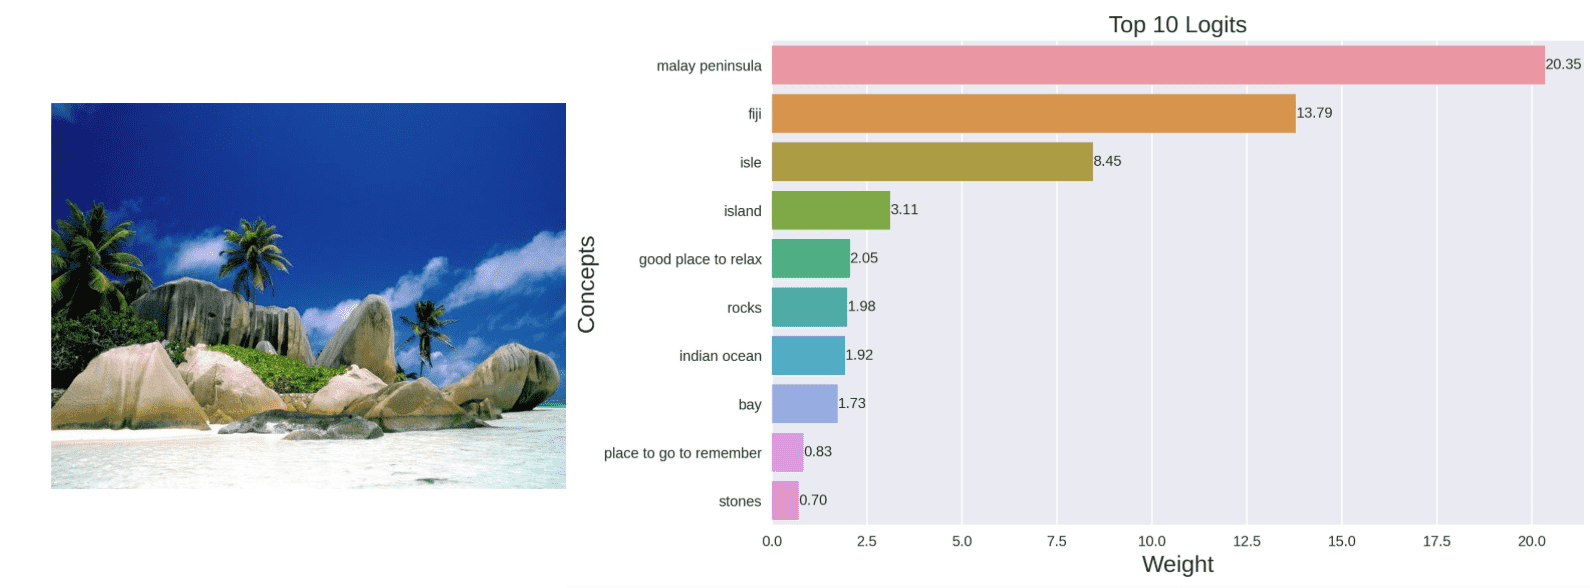
\includegraphics[width=0.75\linewidth]{./figures/sparse_im_1-compressed.png}
    % \caption{Концепты, извлекаемые с помощью Sparse-CBM.}
    \\
    (b) Концепты, извлекаемые с помощью Sparse-CBM.
    % \label{fig:sparse_im_1}
    \end{subfigure}
    \begin{subfigure}%[b]%{3.5cm}
     \centering
  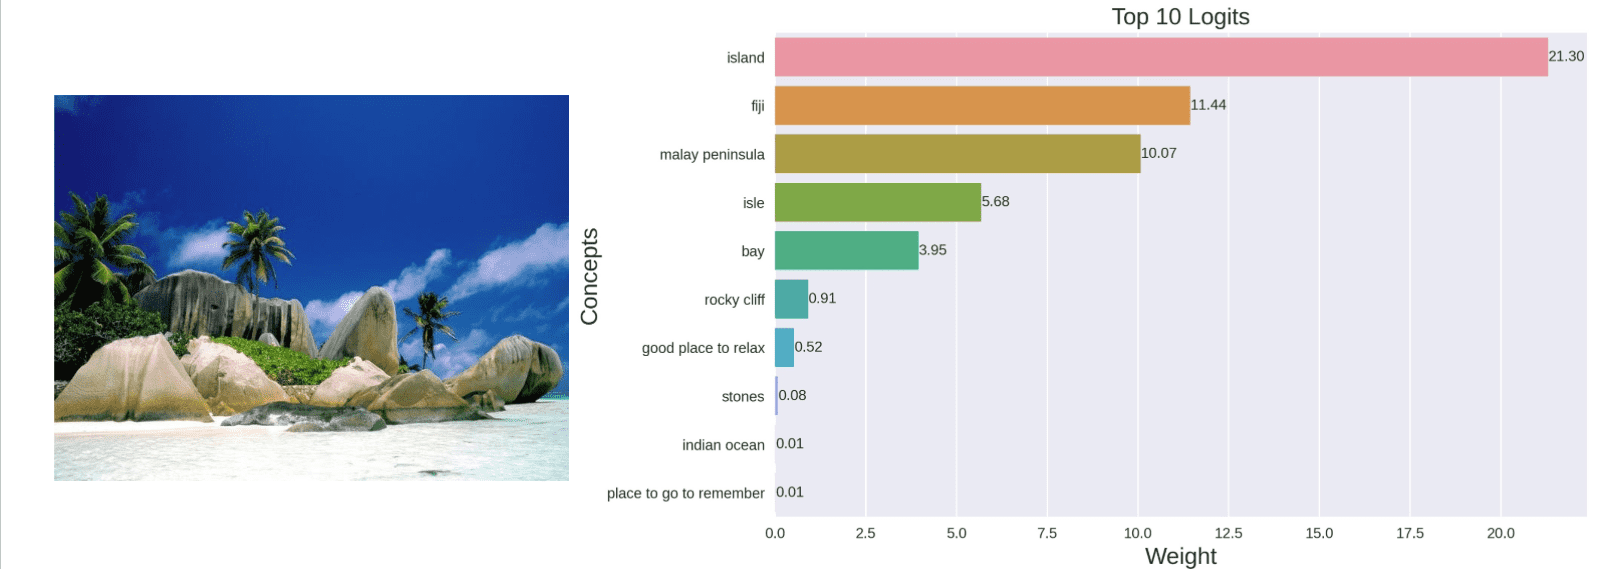
\includegraphics[width=0.75\linewidth]{./figures/l1_im1-compressed.png}
    % \caption{Концепты, извлекаемые с помощью $\ell_1$-CBM.}
    \\
    (c) Концепты, извлекаемые с помощью $\ell_1$-CBM.
    % \label{fig:l1_im_1}
    \end{subfigure}
        \begin{subfigure}%[b]%{3.5cm}
     \centering
  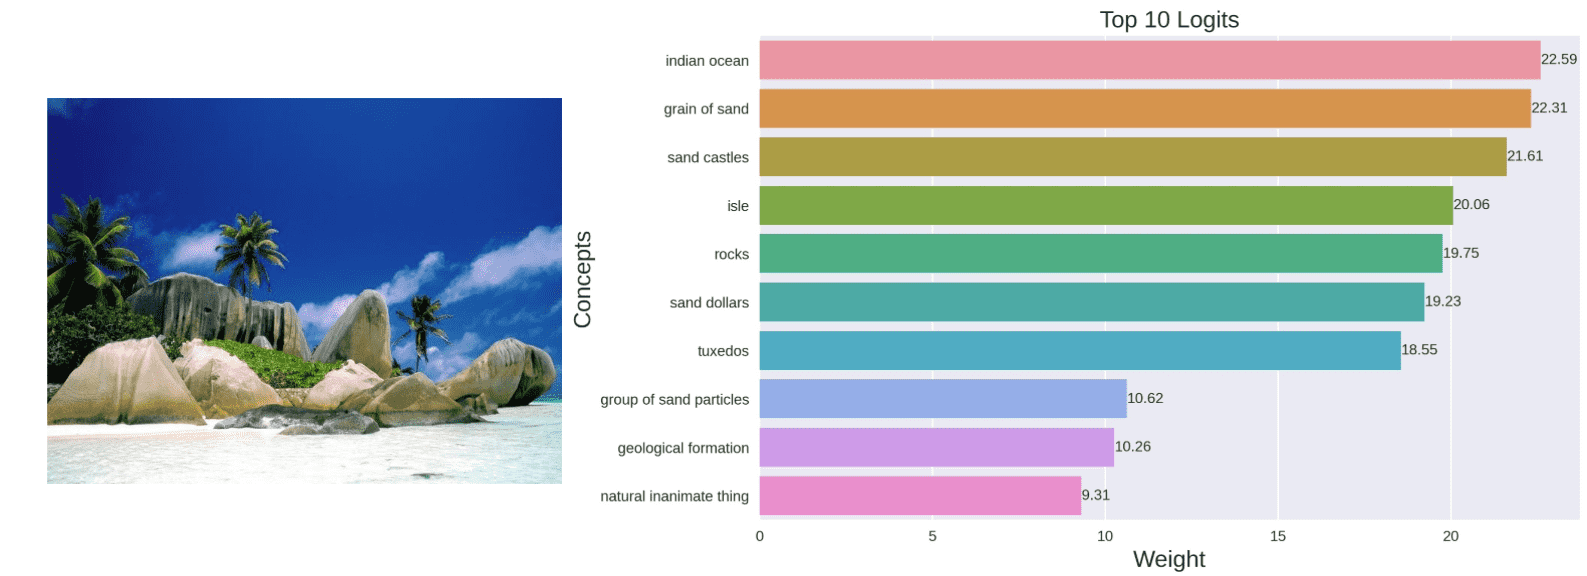
\includegraphics[width=0.75\linewidth]{./figures/contr_im_1-compressed.png}
    % \caption{Концепты, извлекаемые с помощью Contrastive-CBM.}
    \\
    (d) Концепты, извлекаемые с помощью Contrastive-CBM.
    % \label{fig:contr_im_1}
    \end{subfigure}
    \caption{Концепты, извлекаемые с помощью моделей, обученных на Places365.}
    \label{fig:concepts_1}
\end{figure}

\begin{figure}[h] %ht!
\centering
   \begin{subfigure}%[b]%{3.5cm}
     \centering
    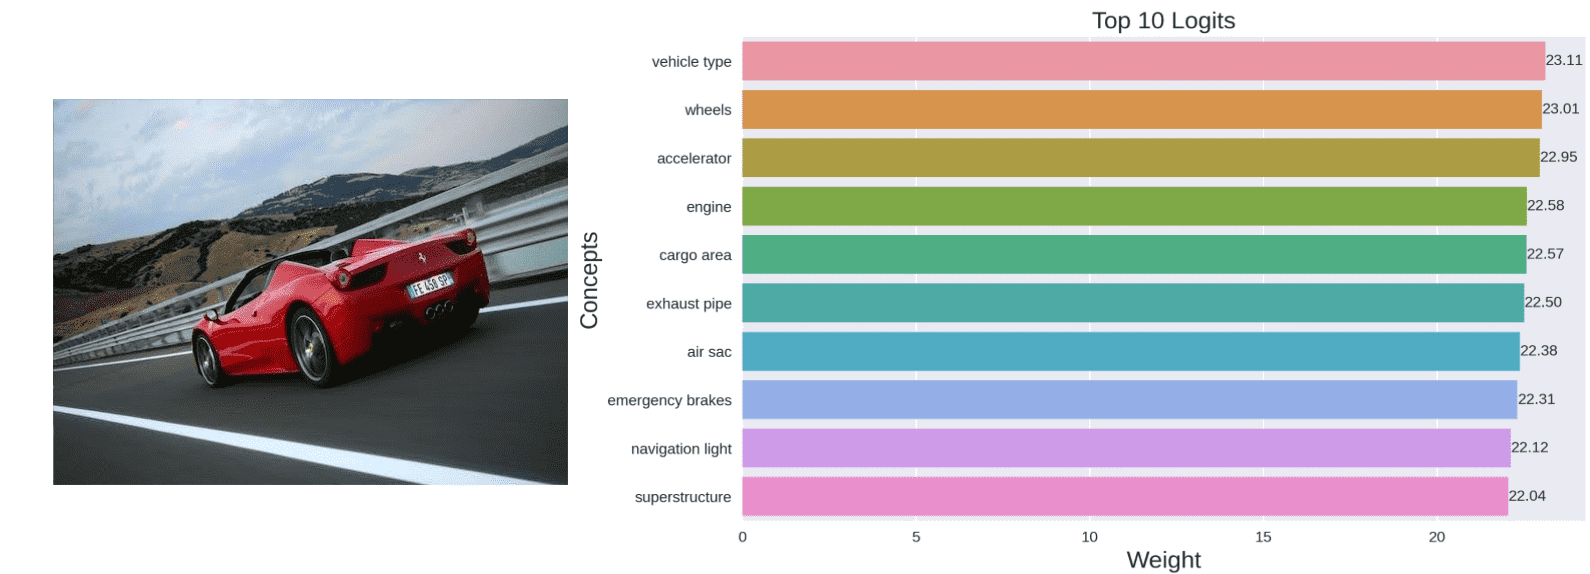
\includegraphics[width=0.75\linewidth]{./figures/clip_im_2-compressed.png}
    % \caption{Концепты, извлекаемые с помощью CLIP.}
    \\
    (a) Концепты, извлекаемые с помощью CLIP.
    % \label{fig:clip_im_2}
    \end{subfigure}
    \begin{subfigure}%[b]%{3.5cm}
    \centering
      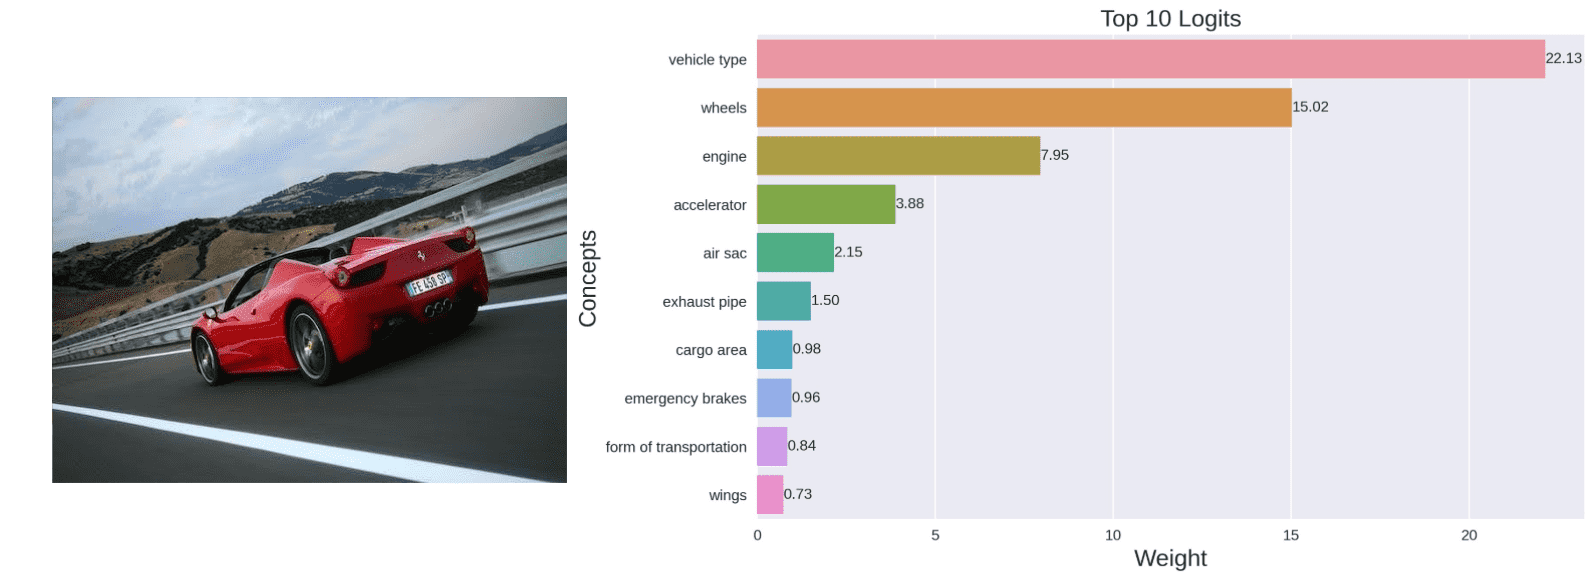
\includegraphics[width=0.75\linewidth]{./figures/sparse_im_2-compressed.png}
    % \caption{Концепты, извлекаемые с помощью Sparse-CBM.}
    \\
    (b) Концепты, извлекаемые с помощью sparse-CBM.
    % \label{fig:sparse_im_2}
    \end{subfigure}
    \begin{subfigure}%[b]%{3.5cm}
     \centering
  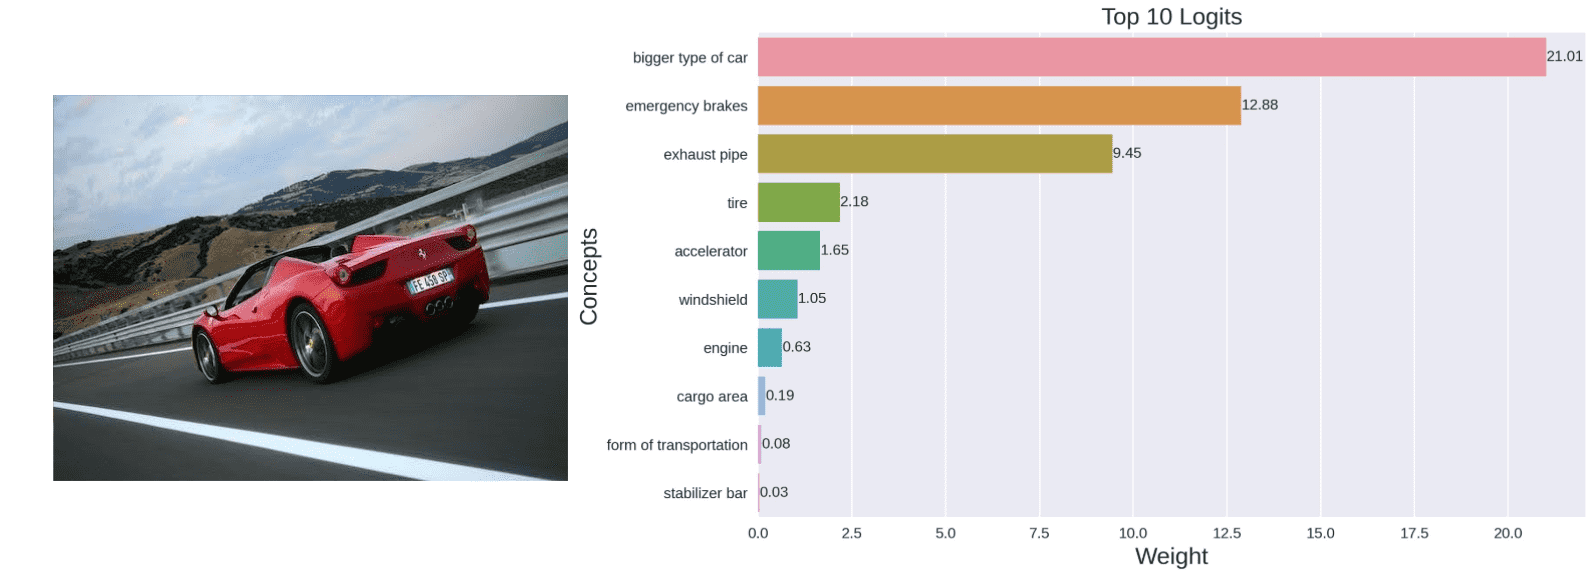
\includegraphics[width=0.75\linewidth]{./figures/l1_im_2-compressed.png}
    % \caption{Концепты, извлекаемые с помощью $\ell_1$-CBM.}
    \\
    (c) Концепты, извлекаемые с помощью $\ell_1$-CBM.
    % \label{fig:l1_im_2}
    \end{subfigure}
        \begin{subfigure}%[b]%{3.5cm}
     \centering
  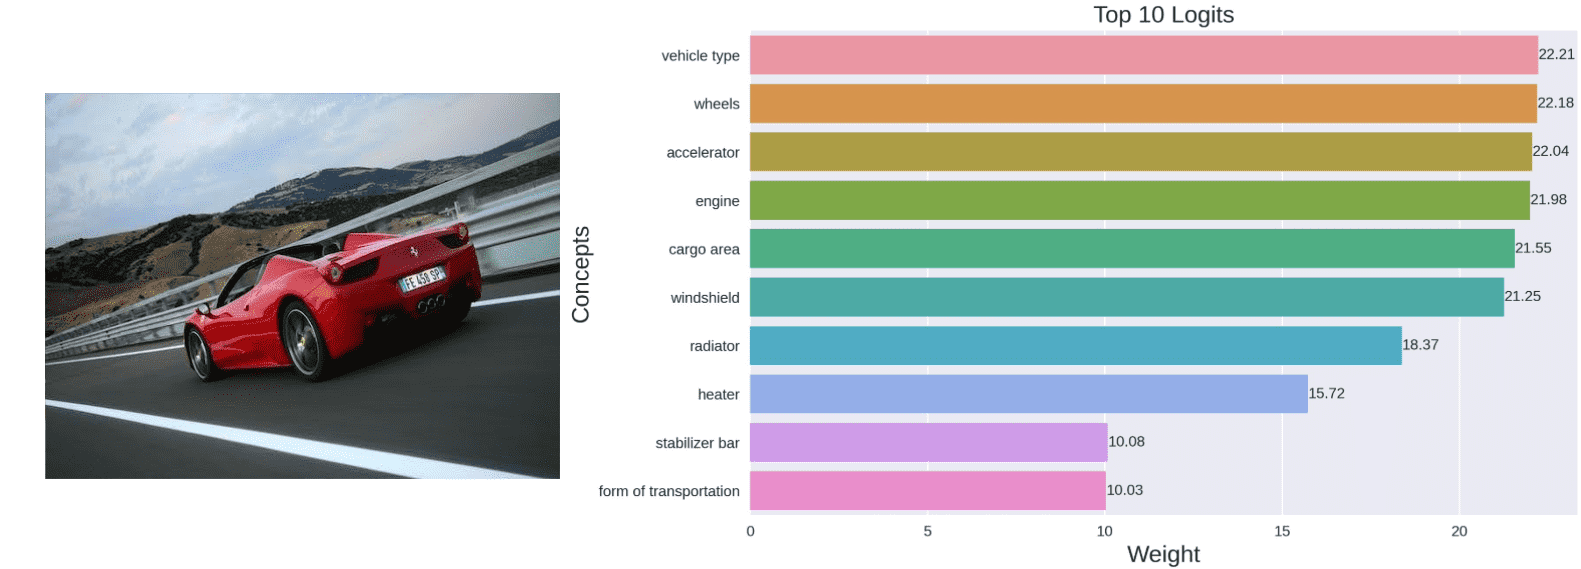
\includegraphics[width=0.75\linewidth]{./figures/contr_im_2-compressed.png}
    % \caption{Концепты, извлекаемые с помощью Contrastive-CBM.}
    \\
    (d) Концепты, извлекаемые с помощью Contrastive-CBM.
    % \label{fig:contr_im_2}
    \end{subfigure}
    \caption{Концепты, извлекаемые с помощью моделей, обученных на CIFAR10.}
    \label{fig:concepts_2}
\end{figure}

\begin{figure}[h] %ht!
\centering
   \begin{subfigure}%[b]%{3.5cm}
     \centering
    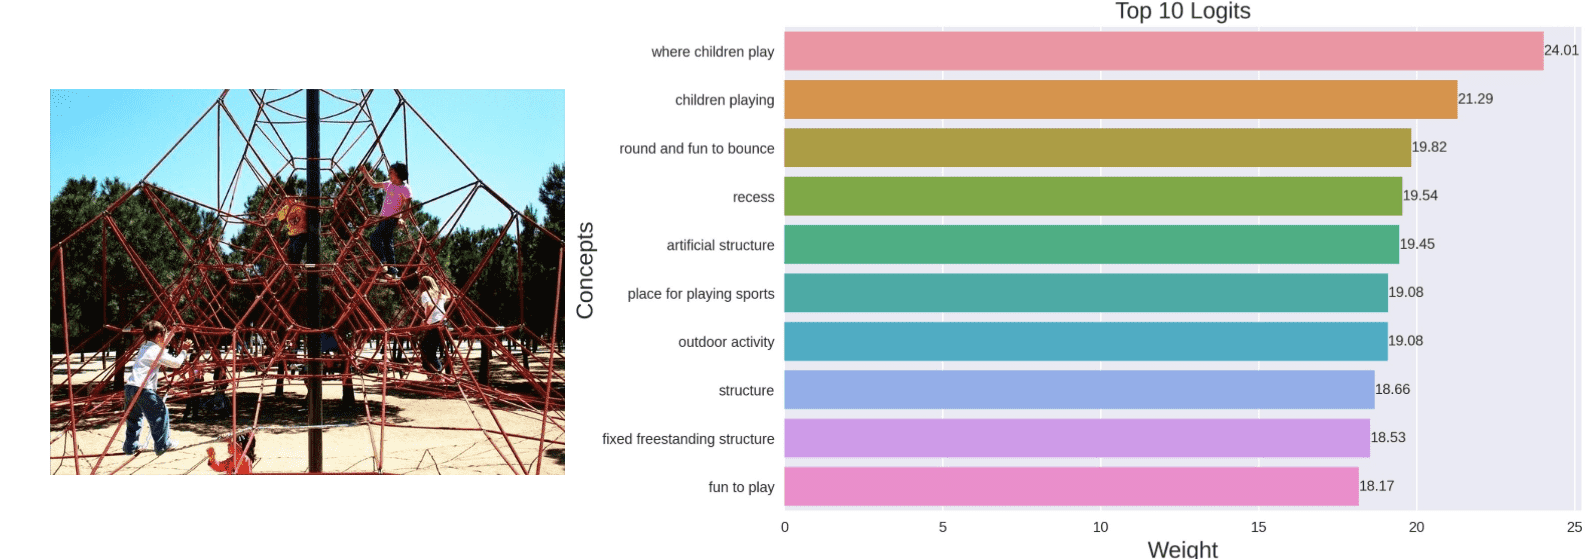
\includegraphics[width=0.75\linewidth]{./figures/clip_im_3-compressed.png}
    % \caption{Концепты, извлекаемые с помощью CLIP.}
    \\
    (a) Концепты, извлекаемые с помощью CLIP.
    % \label{fig:clip_im_3}
    \end{subfigure}
    \begin{subfigure}%[b]%{3.5cm}
    \centering
      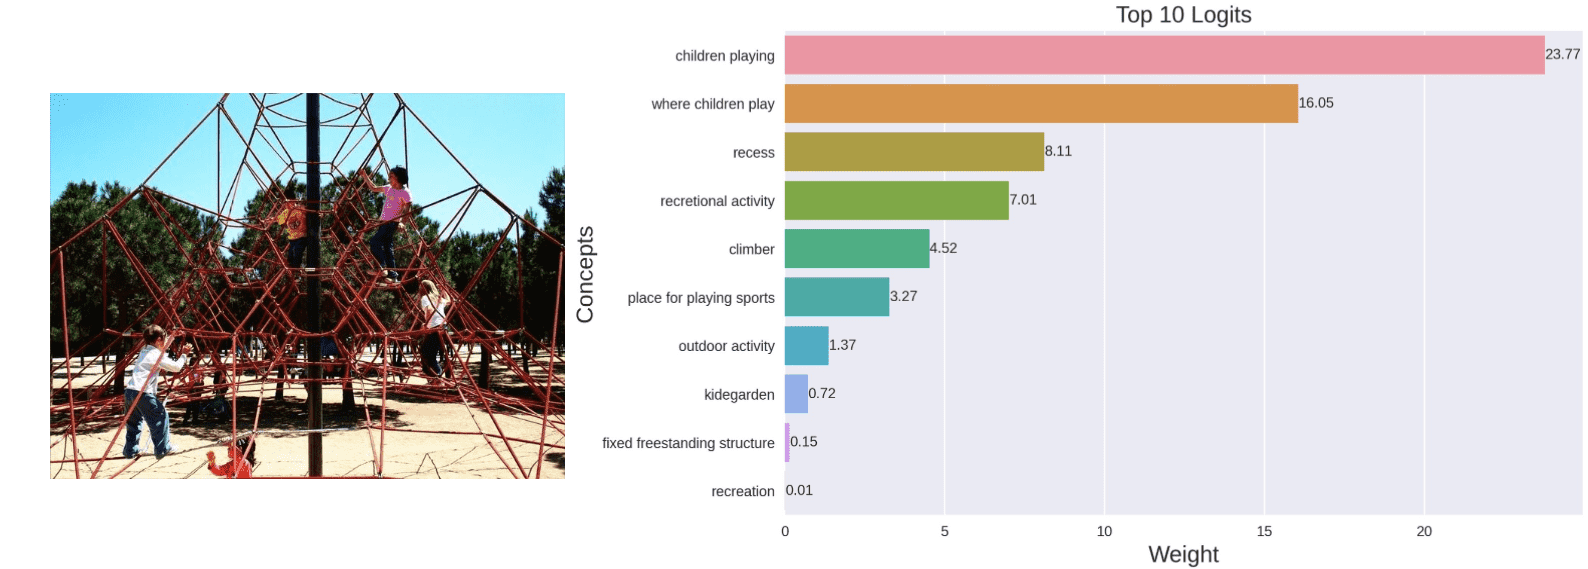
\includegraphics[width=0.75\linewidth]{./figures/sparse_im_3-compressed.png}
    % \caption{Концепты, извлекаемые с помощью Sparse-CBM.}
    \\
    (b) Концепты, извлекаемые с помощью Sparse-CBM.
    % \label{fig:sparse_im_3}
    \end{subfigure}
    \begin{subfigure}%[b]%{3.5cm}
     \centering
  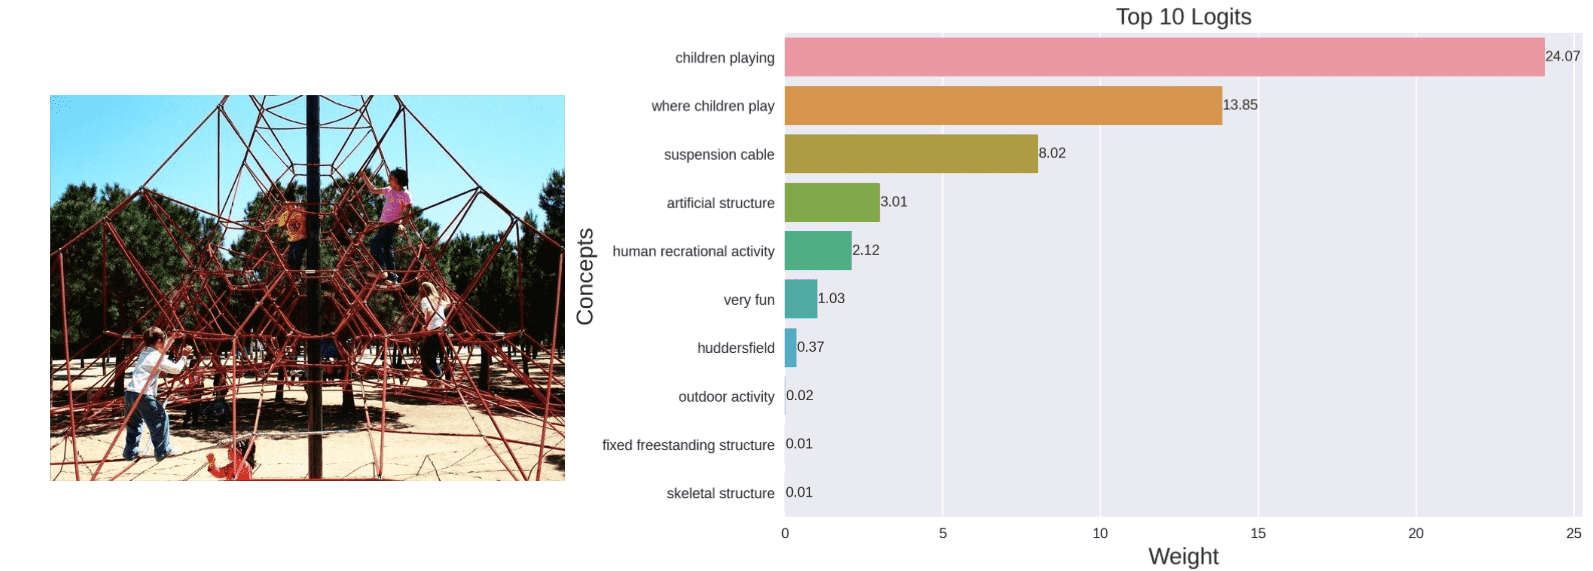
\includegraphics[width=0.75\linewidth]{./figures/l1_im_3-compressed.png}
    % \caption{Концепты, извлекаемые с помощью $\ell_1$-CBM.}
    \\
    (c) Концепты, извлекаемые с помощью $\ell_1$-CBM.
    % \label{fig:l1_im_3}
    \end{subfigure}
        \begin{subfigure}%[b]%{3.5cm}
     \centering
  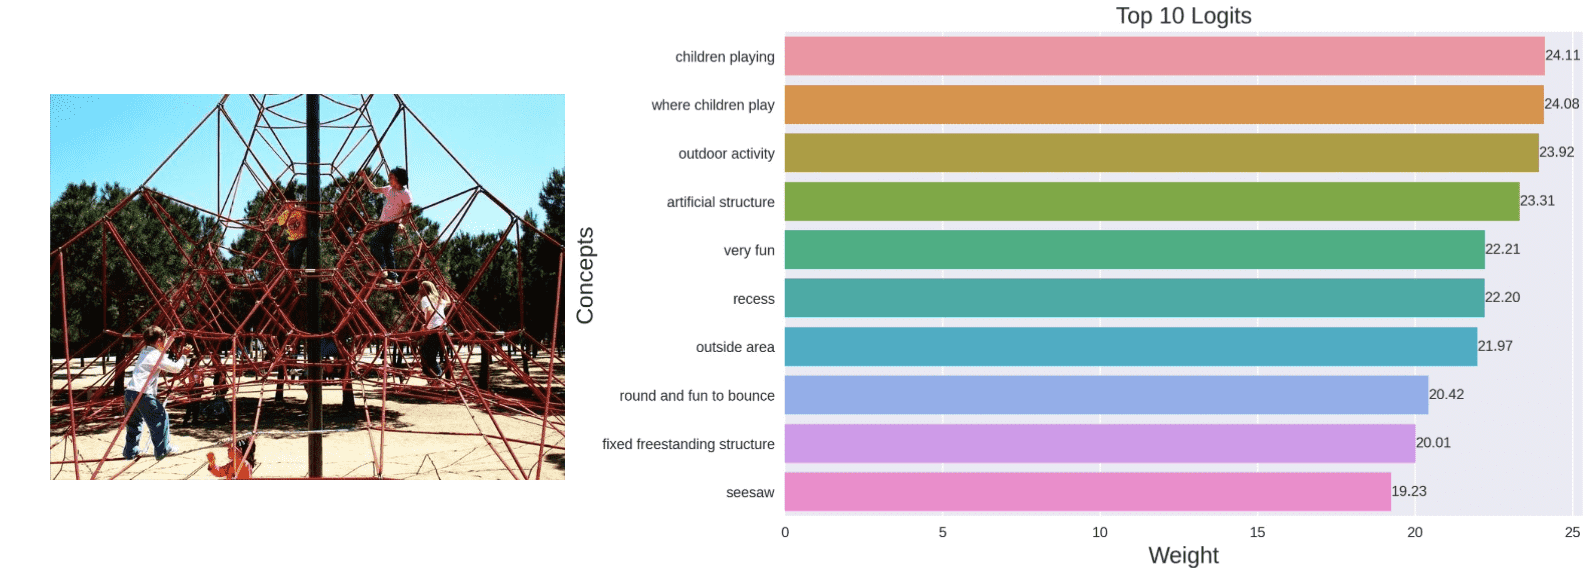
\includegraphics[width=0.75\linewidth]{./figures/contr_im_3-compressed.png}
    % \caption{Концепты, извлекаемые с помощью Contrastive-CBM.}
    \\
    (d) Концепты, извлекаемые с помощью Contrastive-CBM.
    % \label{fig:contr_im_3}
    \end{subfigure}
    \caption{Концепты, извлекаемые с помощью моделей, обученных на Places365.}
    \label{fig:concepts_3}
\end{figure}

\begin{figure}[h] %ht!
\centering
   \begin{subfigure}%[b]%{3.5cm}
     \centering
    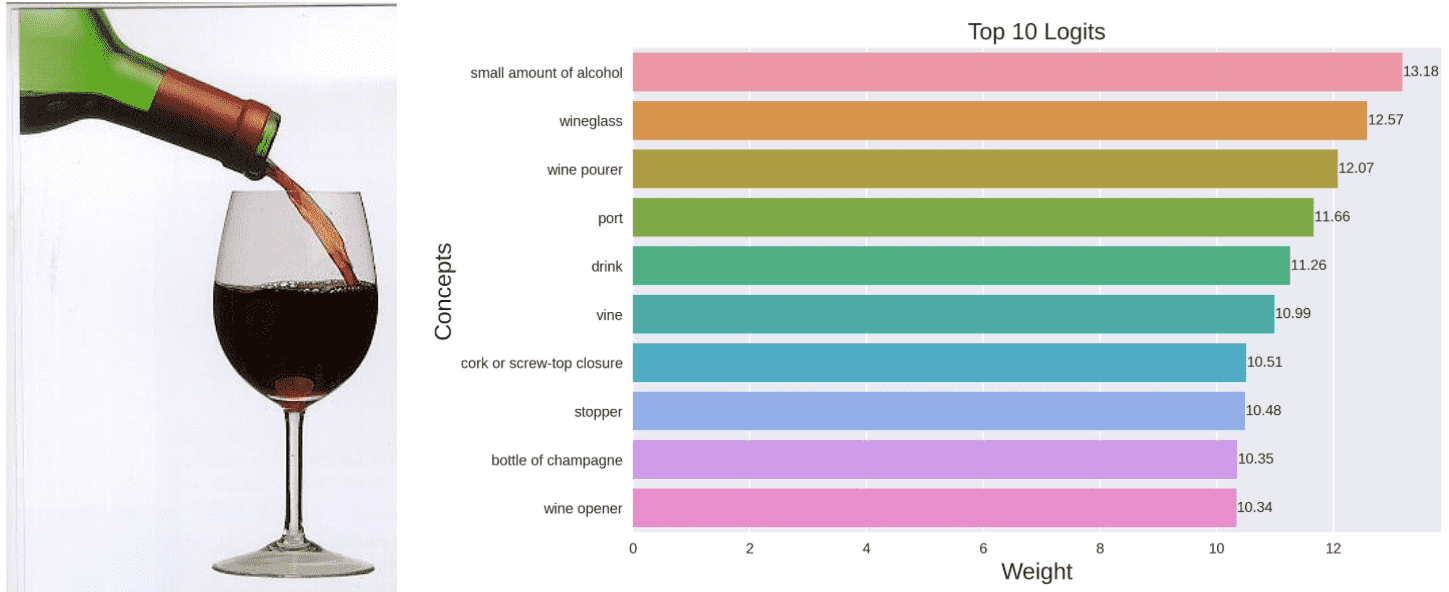
\includegraphics[width=0.65\linewidth]{./figures/clip_im_4-compressed.png}
    % \caption{Концепты, извлекаемые с помощью CLIP.}
    \\
    (a) Концепты, извлекаемые с помощью CLIP.
    % \label{fig:clip_im_4}
    \end{subfigure}
    \begin{subfigure}%[b]%{3.5cm}
    \centering
      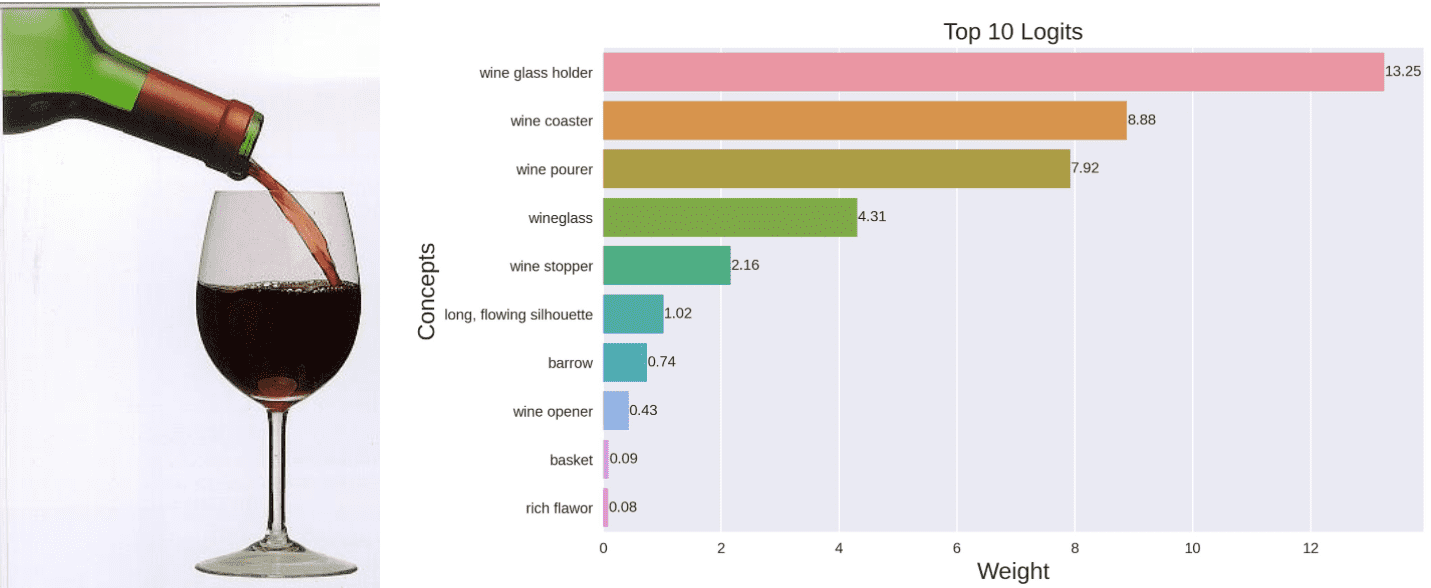
\includegraphics[width=0.65\linewidth]{./figures/sparse_im_4-compressed.png}
    % \caption{Концепты, извлекаемые с помощью Sparse-CBM.}
    \\
    (b) Концепты, извлекаемые с помощью Sparse-CBM.
    % \label{fig:sparse_im_4}
    \end{subfigure}
    \begin{subfigure}%[b]%{3.5cm}
     \centering
  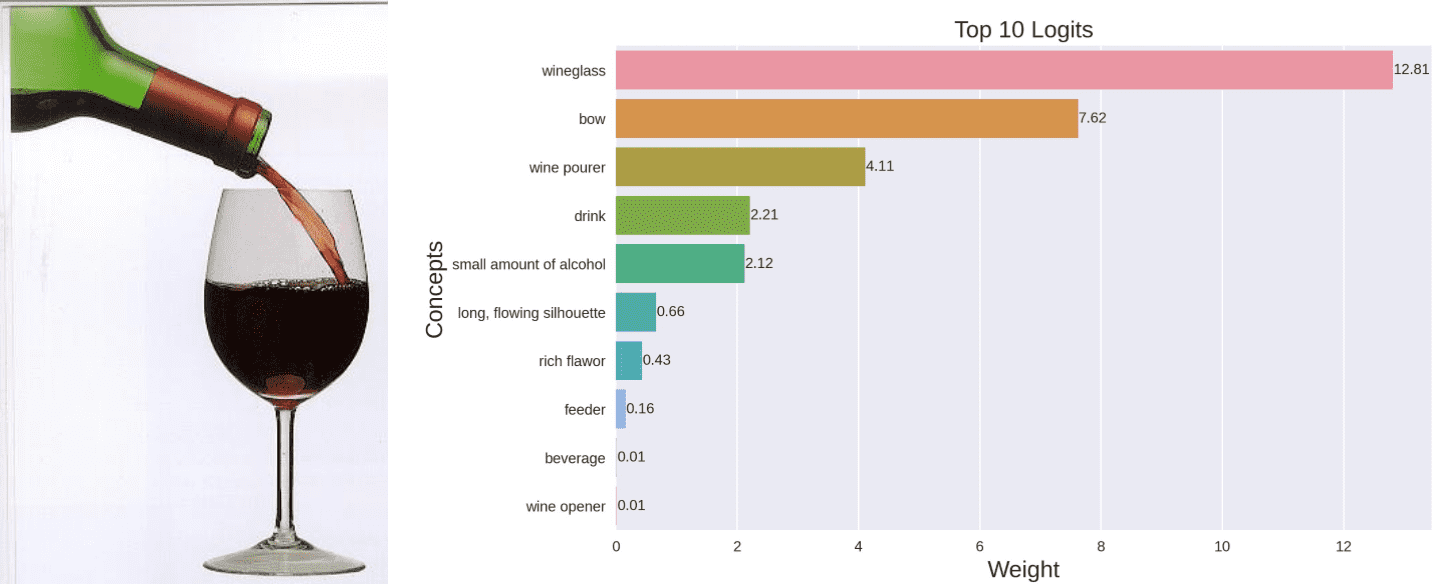
\includegraphics[width=0.65\linewidth]{./figures/l1_im_4-compressed.png}
    % \caption{Концепты, извлекаемые с помощью $\ell_1$-CBM.}
    \\
    (c) Концепты, извлекаемые с помощью $\ell_1$-CBM.
    % \label{fig:l1_im_4}
    \end{subfigure}
        \begin{subfigure}%[b]%{3.5cm}
     \centering
  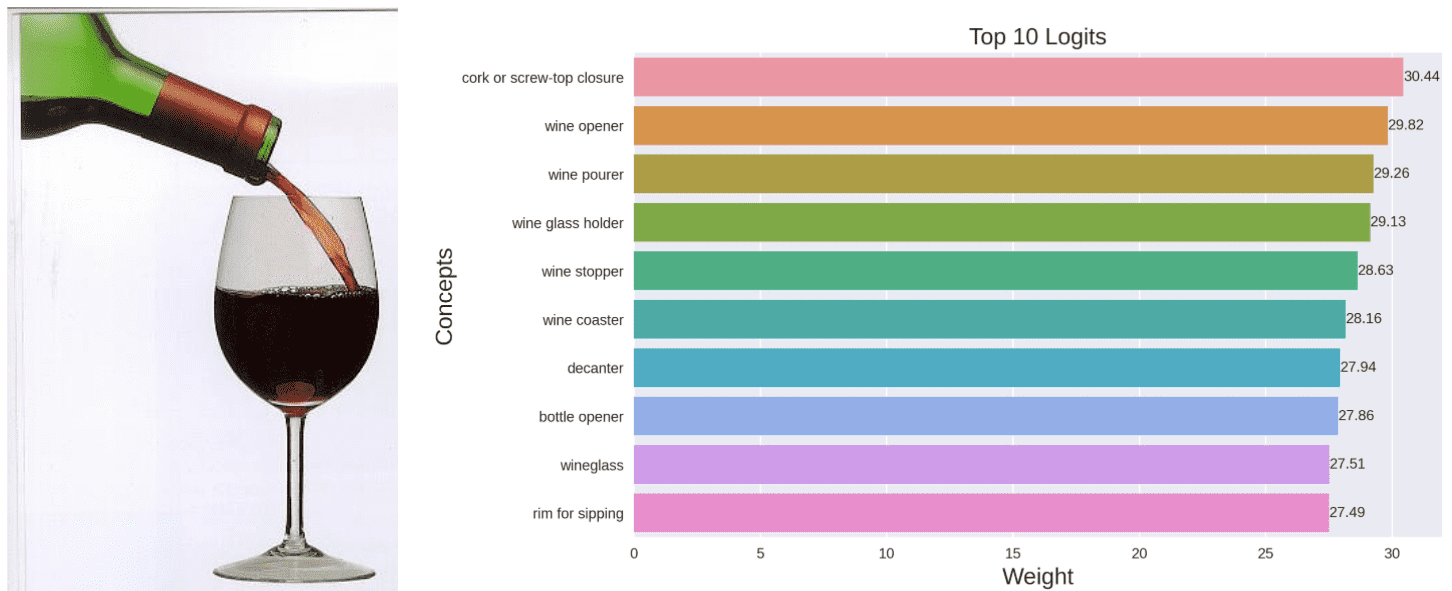
\includegraphics[width=0.65\linewidth]{./figures/contr_im_4-compressed.png}
    % \caption{Концепты, извлекаемые с помощью Contrastive-CBM.}
    \\
    (d) Концепты, извлекаемые с помощью Contrastive-CBM.
    % \label{fig:contr_im_4}
    \end{subfigure}
    \caption{Концепты, извлекаемые с помощью моделей, обученных на ImageNet.}
    \label{fig:concepts_4}
\end{figure}

\begin{figure}[h] %ht!
\centering
   \begin{subfigure}%[b]%{3.5cm}
     \centering
    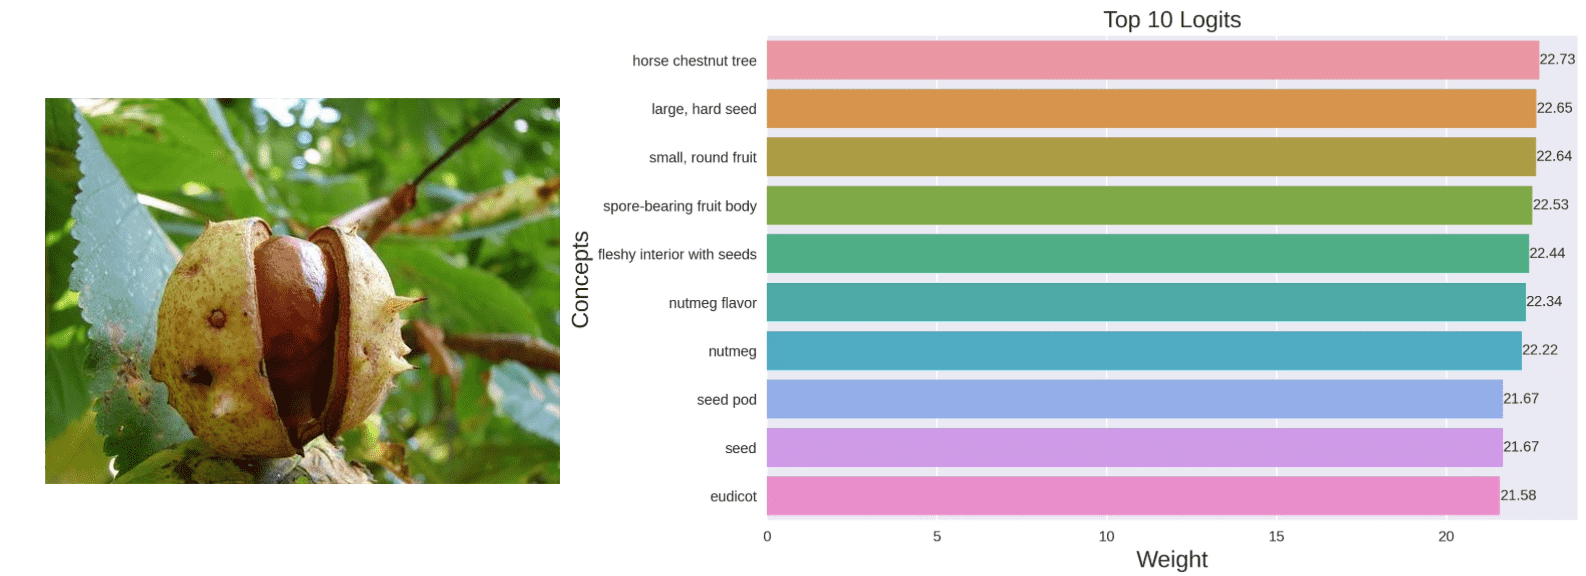
\includegraphics[width=0.7\linewidth]{./figures/clip_im_5-compressed.png}
    % \caption{Концепты, извлекаемые с помощью CLIP.}
    \\
    (a) Концепты, извлекаемые с помощью CLIP.
    % \label{fig:clip_im_5}
    \end{subfigure}
    \begin{subfigure}%[b]%{3.5cm}
    \centering
      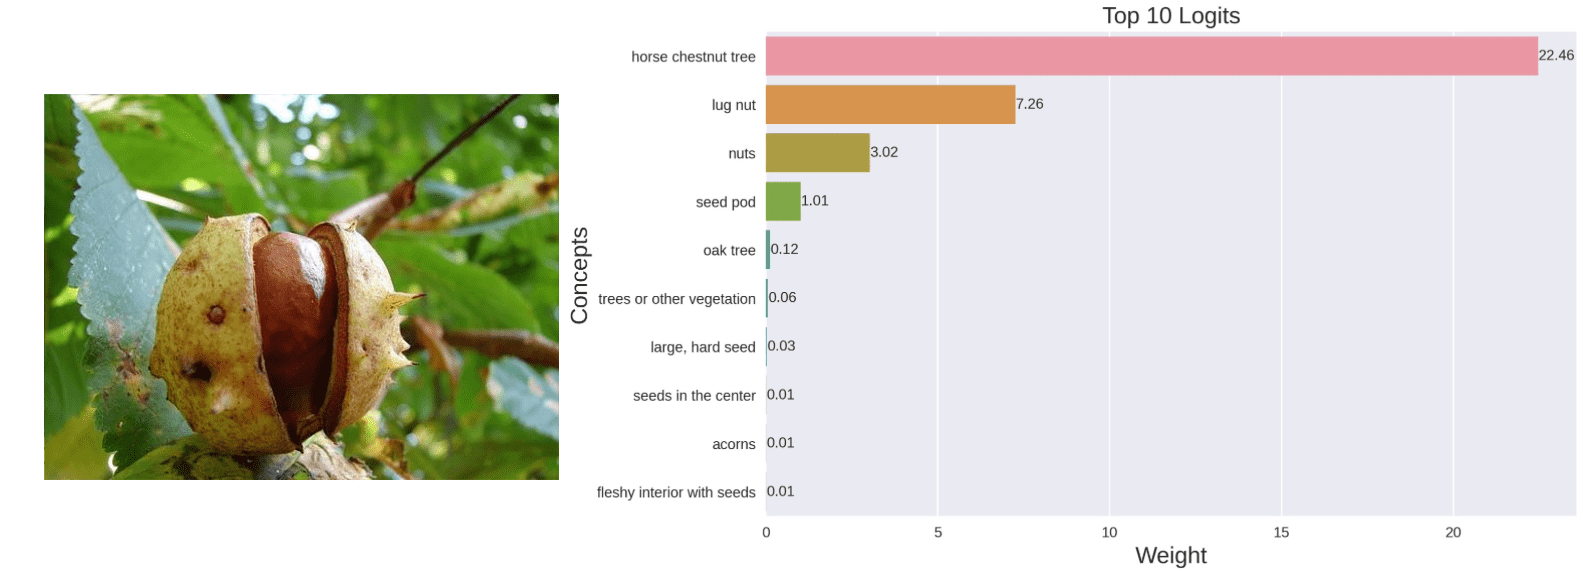
\includegraphics[width=0.7\linewidth]{./figures/sparse_im_5-compressed.png}
    % \caption{Концепты, извлекаемые с помощью Sparse-CBM.}
    \\
    (b) Концепты, извлекаемые с помощью Sparse-CBM.
    % \label{fig:sparse_im_5}
    \end{subfigure}
    \begin{subfigure}%[b]%{3.5cm}
     \centering
  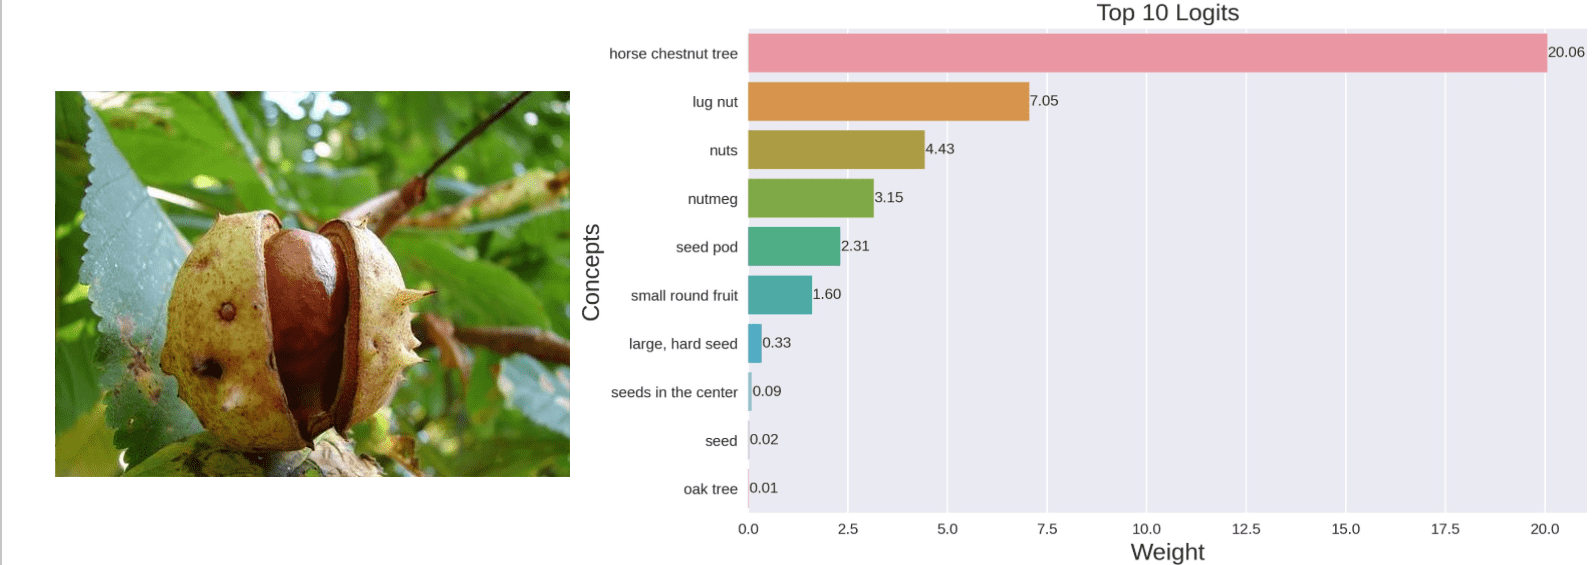
\includegraphics[width=0.75\linewidth]{./figures/l1_im_5-compressed.png}
    % \caption{Концепты, извлекаемые с помощью $\ell_1$-CBM.}
    \\
    (c) Концепты, извлекаемые с помощью $\ell_1$-CBM.
    % \label{fig:l1_im_5}
    \end{subfigure}
        \begin{subfigure}%[b]%{3.5cm}
     \centering
  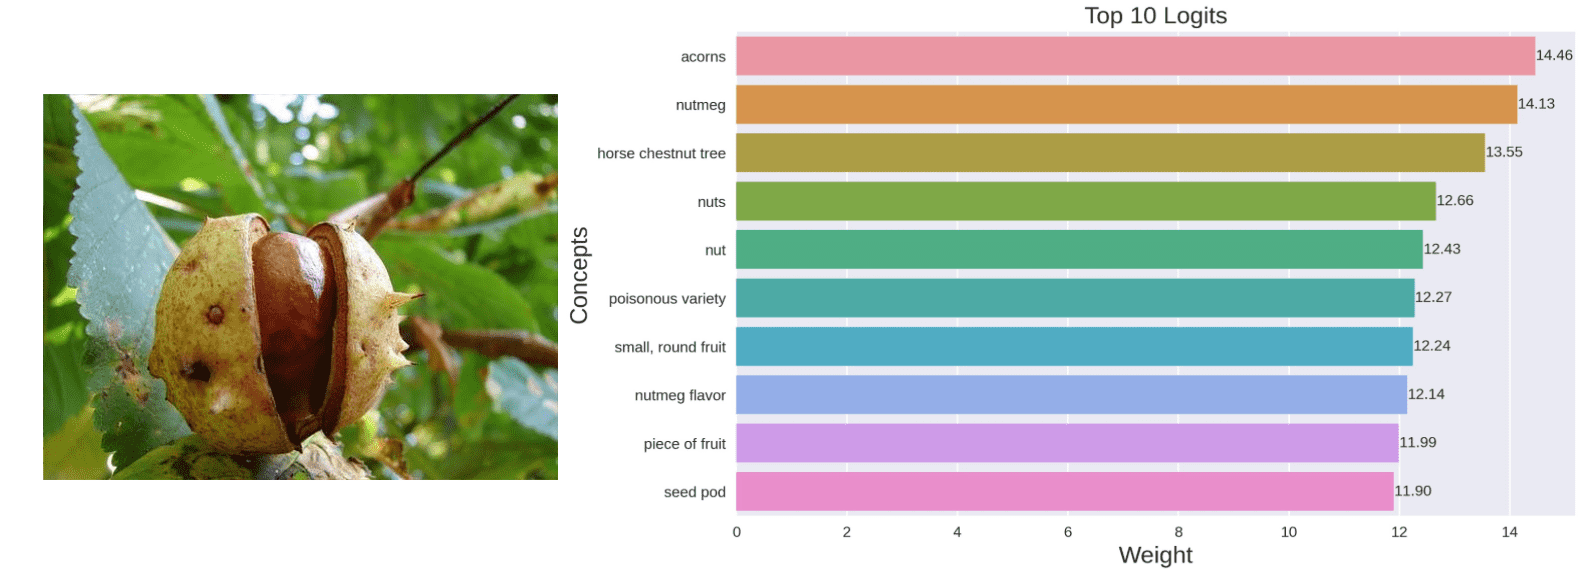
\includegraphics[width=0.75\linewidth]{./figures/contr_im_5-compressed.png}
    % \caption{Концепты, извлекаемые с помощью Contrastive-CBM.}
    \\
    (d) Концепты, извлекаемые с помощью Contrastive-CBM.
    % \label{fig:contr_im_5}
    \end{subfigure}
    \caption{Концепты, извлекаемые с помощью моделей, обученных на Places365.}
    \label{fig:concepts_5}
\end{figure}

\begin{figure}[h] %ht!
\centering
   \begin{subfigure}%[b]%{3.5cm}
     \centering
    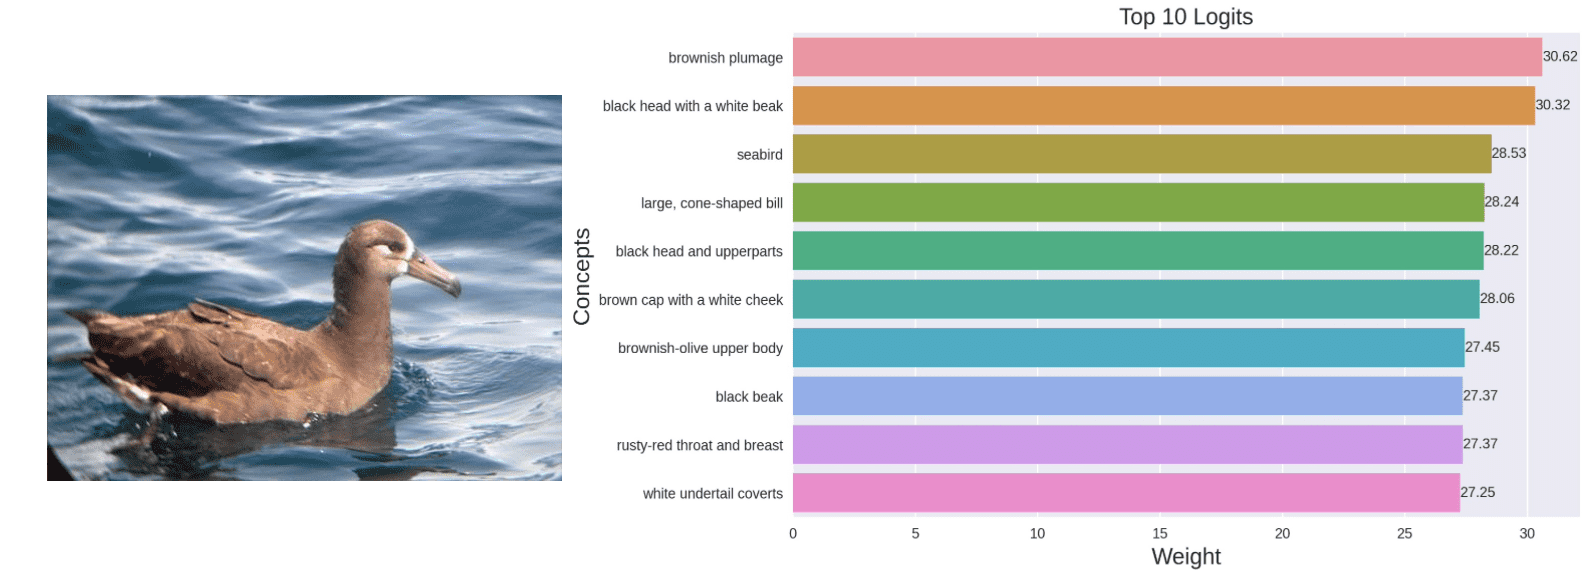
\includegraphics[width=0.75\linewidth]{./figures/clip_im_6-compressed.png}
    % \caption{Концепты, извлекаемые с помощью CLIP.}
    \\
    (a) Концепты, извлекаемые с помощью CLIP.
    % \label{fig:clip_im_6}
    \end{subfigure}
    \begin{subfigure}%[b]%{3.5cm}
    \centering
      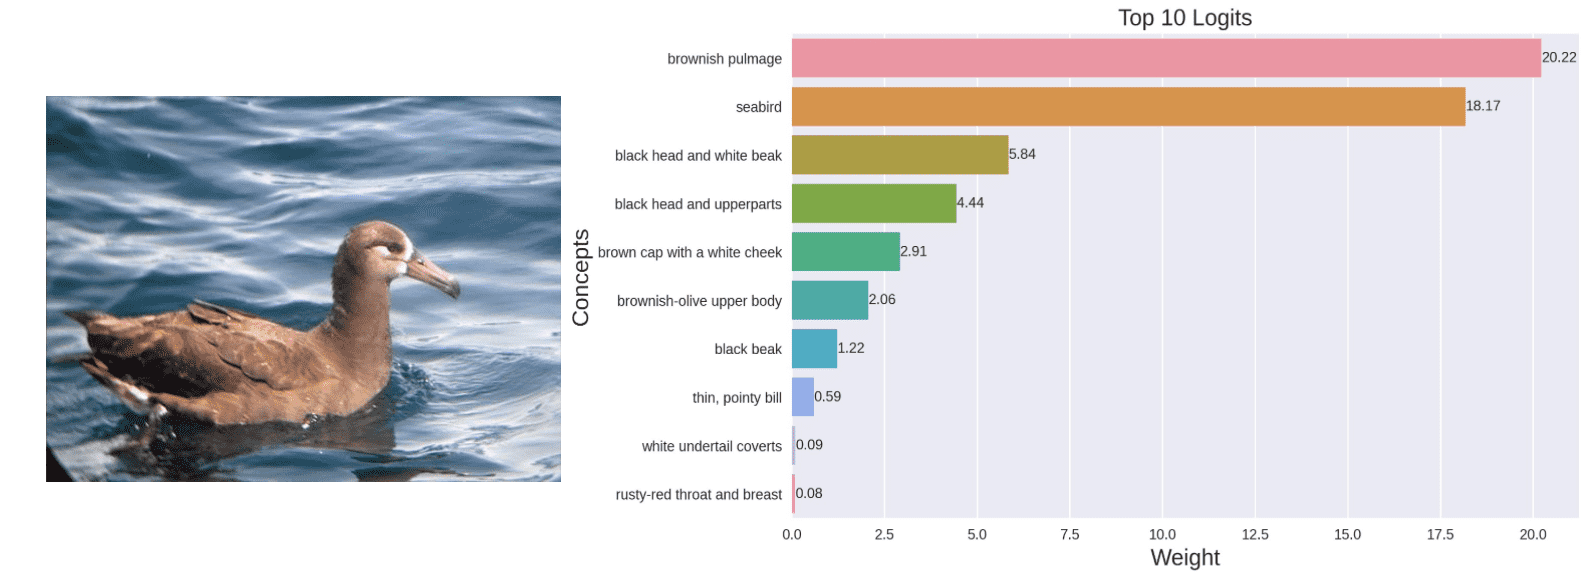
\includegraphics[width=0.75\linewidth]{./figures/sparse_im_6-compressed.png}
    % \caption{Концепты, извлекаемые с помощью Sparse-CBM.}
    \\
    (b) Концепты, извлекаемые с помощью Sparse-CBM.
    % \label{fig:sparse_im_6}
    \end{subfigure}
    \begin{subfigure}%[b]%{3.5cm}
     \centering
  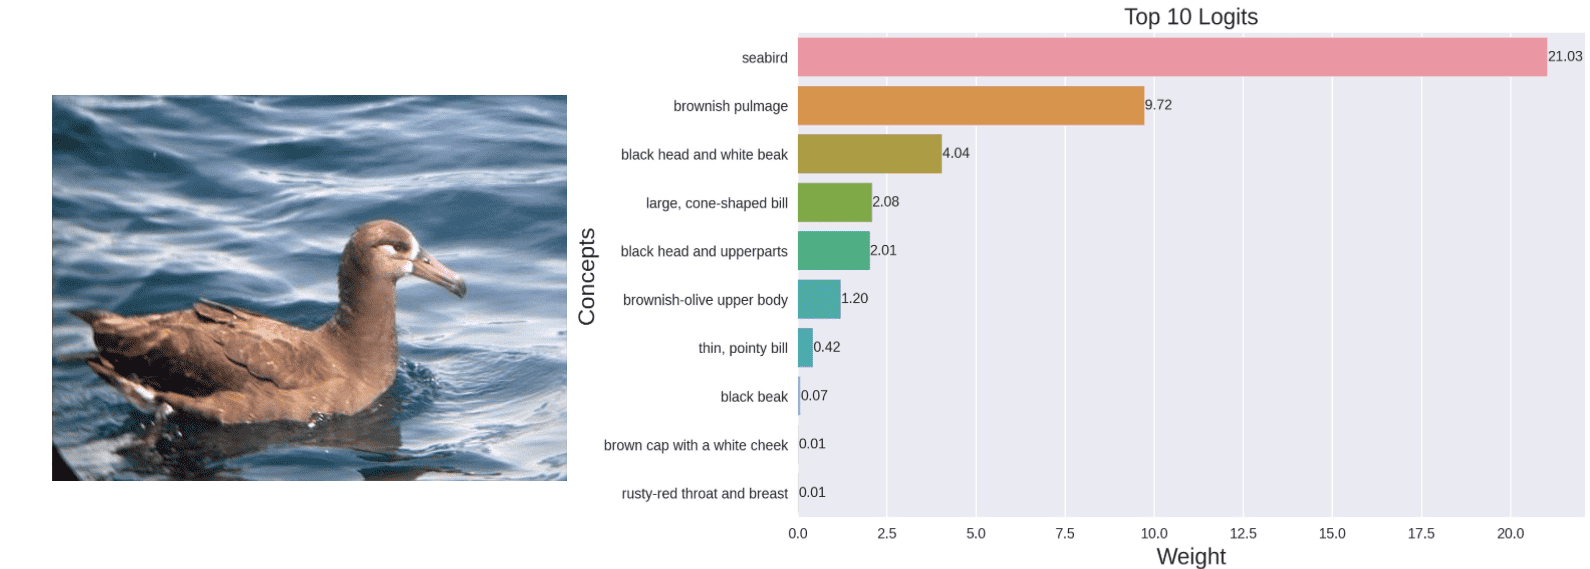
\includegraphics[width=0.75\linewidth]{./figures/l1_im_6-compressed.png}
    % \caption{Концепты, извлекаемые с помощью $\ell_1$-CBM.}
    \\
    (c) Концепты, извлекаемые с помощью $\ell_1$-CBM.
    % \label{fig:l1_im_6}
    \end{subfigure}
        \begin{subfigure}%[b]%{3.5cm}
     \centering
  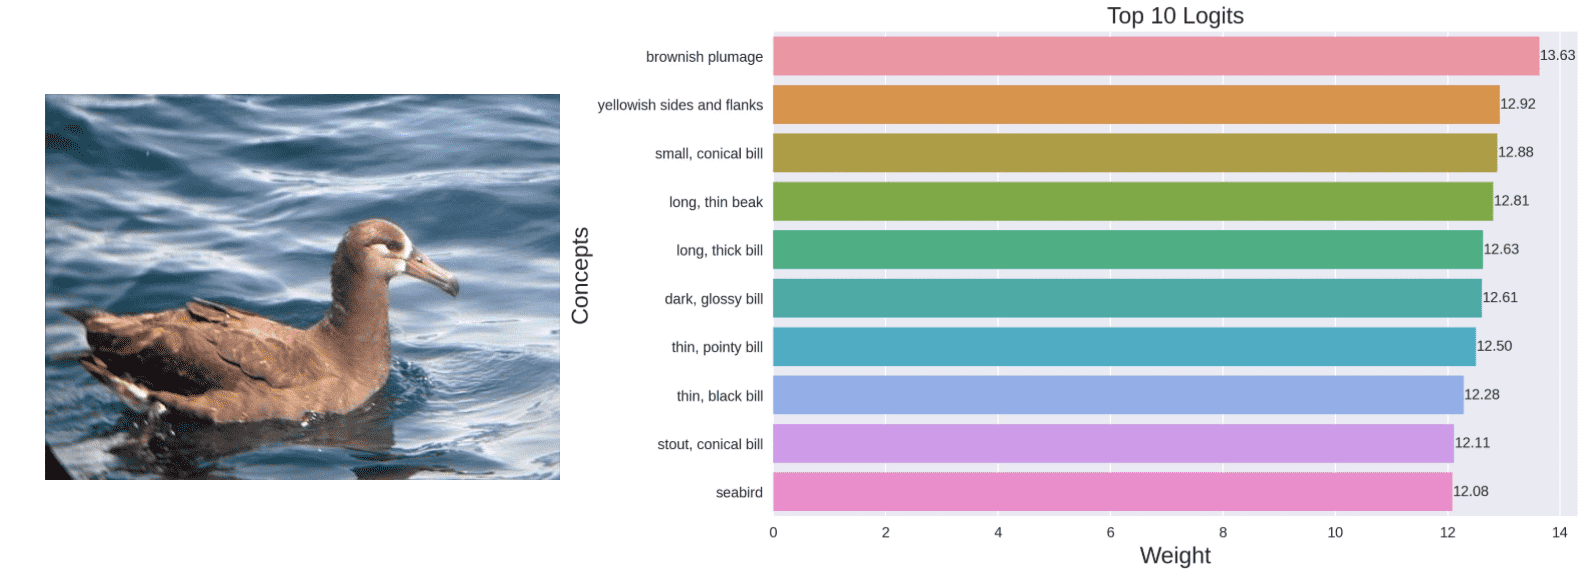
\includegraphics[width=0.75\linewidth]{./figures/contr_im_6-compressed.png}
    % \caption{Концепты, извлекаемые с помощью Contrastive-CBM.}
    \\
    (d) Концепты, извлекаемые с помощью Contrastive-CBM.
    % \label{fig:contr_im_6}
    \end{subfigure}
    \caption{Концепты, извлекаемые с помощью моделей, обученных на CUB200.}
    \label{fig:concepts_6}
\end{figure}

\subsection{Sparse-CBM ошибки}
\label{sec:sparse_confusion}
Вместе с итоговыми результатами классификации мы приводим матрицу путаницы лучшей Sparse-CBM, обученной на наборе данных CUB200, которая достигает 80,02\% точности в \cref{fig:cub_conf_matrix}. Следует заметить, что наиболее значительные ошибки модели закладываются в последней части меток. Сюда входят несколько схожих классов, таких как "черношапочный вирео", "синеголовый вирео", "филадельфийский вирео", "красноглазый вирео", "певчий вирео", "белоглазый вирео" и "желтоголовый вирео". В целом, в таких разнообразных наборах данных, как CUB200, представлено множество схожих классов, поэтому имеет смысл рассмотреть возможность выделения понятий и подчеркнуть их различия между такими классами, как "красноглазый вирео" и "белоглазый вирео".

\begin{figure}[t]%{l}{0.25\textwidth}
\begin{center}
\centerline{
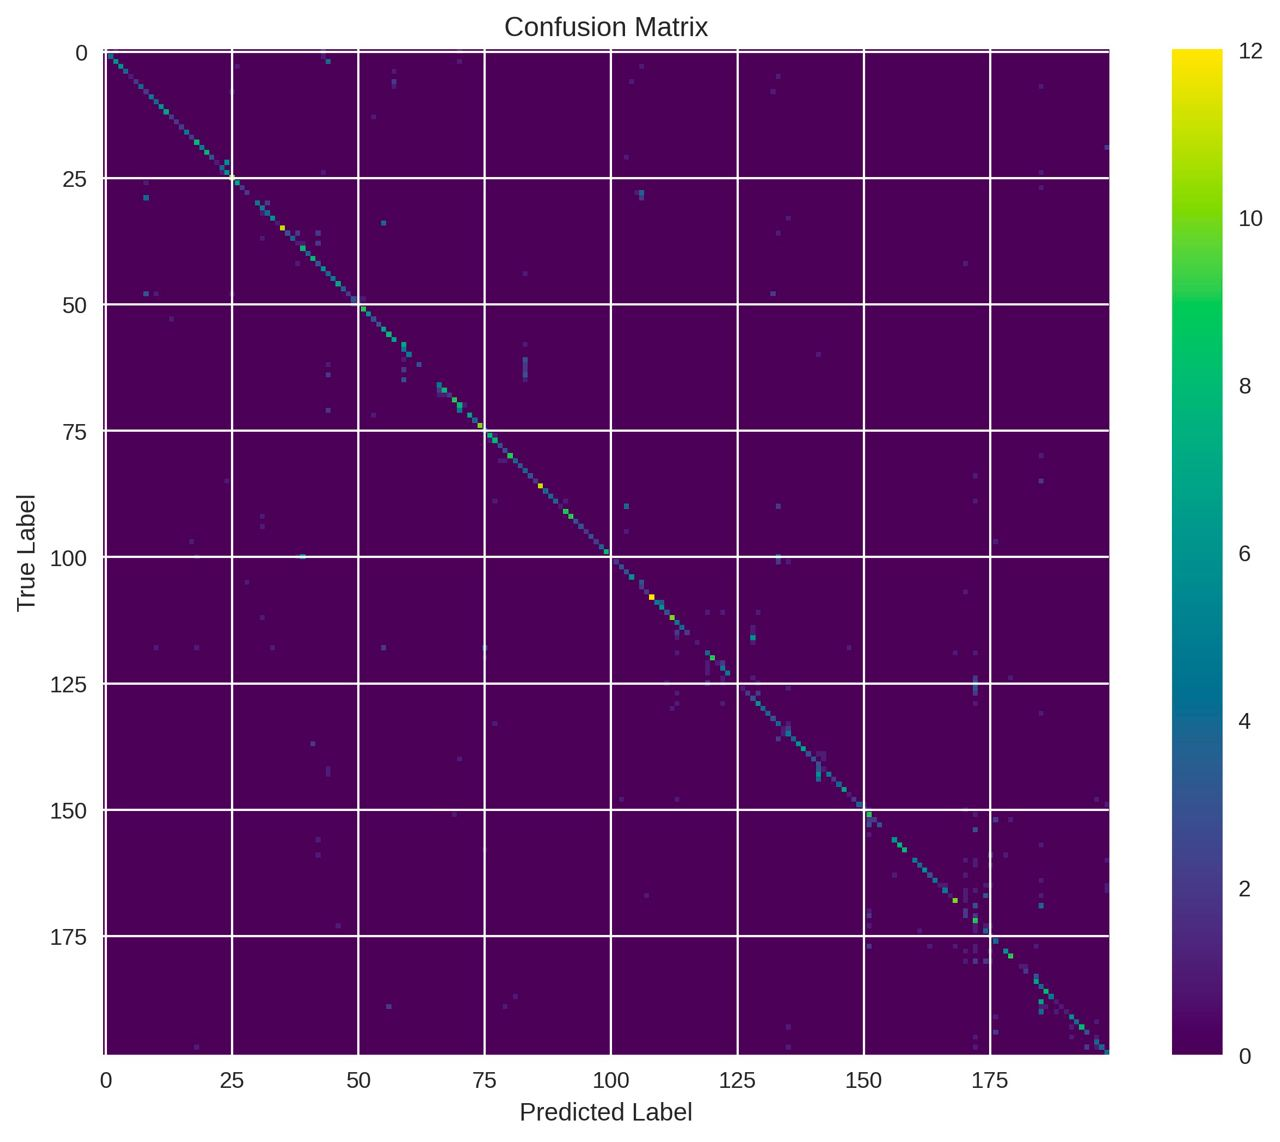
\includegraphics[width=0.6\columnwidth]{./figures/cub_conf_matrix.jpg}}
\caption{Матрица ошибок Sparse-CBM на наборе данных CUB200.}
\label{fig:cub_conf_matrix}
\end{center}
\end{figure}
\end{document}
